\documentclass[11pt]{article}

% ==================================================
% Page layout
% ==================================================
\usepackage[a4paper,margin=1in]{geometry}

\setlength{\parskip}{0.35em}
\setlength{\parindent}{0pt}

% ==================================================
% Mathematics
% ==================================================
\usepackage{amsmath,amssymb,amsthm,mathtools,bm}

% ==================================================
% Typography, lists, tables, and graphics
% ==================================================
\usepackage[protrusion=true,expansion=false]{microtype}
\usepackage{enumitem}
\usepackage{booktabs}
\usepackage{graphicx}
\usepackage{xcolor}
\usepackage{float}

% ==================================================
% Algorithms
% ==================================================
\usepackage{algorithm}
\usepackage[noend]{algpseudocode}

% ==================================================
% Bibliography
% ==================================================
\usepackage[round,authoryear]{natbib}

% ==================================================
% TikZ and PGFPlots
% ==================================================
\usepackage{tikz}
\usetikzlibrary{
arrows.meta,
positioning,
calc,
backgrounds,
fit
}

\usepackage{pgfplots}
\pgfplotsset{compat=1.17}

% ==================================================
% Colored boxes
% ==================================================
\usepackage[most]{tcolorbox}
\usepackage{subcaption}

% ==================================================
% Hyperlinks
% ==================================================
\usepackage[
colorlinks=true,
linkcolor=black,
citecolor=blue!55!black,
urlcolor=blue!55!black
]{hyperref}

% ==================================================
% Theorem environments
% ==================================================
\theoremstyle{plain}
\newtheorem{theorem}{Theorem}
\newtheorem{lemma}{Lemma}
\newtheorem{proposition}{Proposition}
\newtheorem{corollary}{Corollary}

\theoremstyle{definition}
\newtheorem{assumption}{Assumption}
\newtheorem{definition}{Definition}

\theoremstyle{remark}
\newtheorem{remark}{Remark}

% ==================================================
% Mathematical macros
% ==================================================
\newcommand{\X}{\mathcal{X}}
\newcommand{\D}{\mathcal{D}}
\newcommand{\C}{\mathcal{C}}
\newcommand{\GP}{\mathcal{GP}}
\newcommand{\N}{\mathcal{N}}
\newcommand{\R}{\mathbb{R}}
\newcommand{\E}{\mathbb{E}}
\newcommand{\Prob}{\mathbb{P}}
\newcommand{\KL}{\mathrm{KL}}

\newcommand{\acq}{a}
\newcommand{\regret}{\mathrm{Reg}}

\newcommand{\bx}{\mathbf{x}}
\newcommand{\bk}{\mathbf{k}}
\newcommand{\bK}{\mathbf{K}}
\newcommand{\by}{\mathbf{y}}
\newcommand{\br}{\mathbf{r}}
\newcommand{\mvec}{\mathbf{m}}

\newcommand{\xhat}{\hat{x}}
\newcommand{\xstar}{x^{\star}}

\DeclareMathOperator*{\argmax}{arg\,max}
\DeclareMathOperator*{\argmin}{arg\,min}

% ==================================================
% Author comments
% ==================================================
\newcommand{\jun}[1]{\textcolor{red}{[Jun: #1]}}
\newcommand{\anjie}[1]{\textcolor{blue}{[Anjie: #1]}}
\newcommand{\bob}[1]{\textcolor{teal}{[Bob: #1]}}

% ==================================================
% General color palette
% ==================================================
\definecolor{knownblue}{RGB}{221,235,247}
\definecolor{uncertainorange}{RGB}{252,229,205}
\definecolor{latentgreen}{RGB}{226,239,218}
\definecolor{unknowngray}{RGB}{238,238,238}

\definecolor{deepblue}{RGB}{45,92,136}
\definecolor{deeporange}{RGB}{174,92,28}
\definecolor{deepgreen}{RGB}{63,117,65}
\definecolor{deepgray}{RGB}{85,85,85}

\definecolor{chatred}{RGB}{247,214,214}
\definecolor{chatredline}{RGB}{193,66,66}
\definecolor{chatdeep}{RGB}{140,38,38}
\definecolor{chathdr}{RGB}{233,182,182}

\definecolor{reasonblue}{RGB}{210,228,246}
\definecolor{reasonblueline}{RGB}{52,104,160}
\definecolor{reasondeep}{RGB}{30,66,110}
\definecolor{reasonhdr}{RGB}{180,208,238}

\definecolor{discgreen}{RGB}{221,237,212}
\definecolor{discgreenline}{RGB}{58,112,60}
\definecolor{discdeep}{RGB}{34,74,36}
\definecolor{dischdr}{RGB}{194,224,184}

\definecolor{axisgray}{RGB}{120,120,120}
\definecolor{bodygray}{RGB}{55,55,55}

% ==================================================
% Pale-red title-card colors
% ==================================================
\definecolor{ldmred}{HTML}{A33A3A}
\definecolor{ldmdarkred}{HTML}{7F2929}
\definecolor{ldmtext}{HTML}{282323}
\definecolor{ldmbg}{HTML}{FBF5F5}
\definecolor{ldmedge}{HTML}{E8D3D3}

% ==================================================
% Document
% ==================================================
\begin{document}

% Do not use \maketitle here.
% The title, authors, affiliations, and abstract are
% placed directly inside this tcolorbox.

\begin{tcolorbox}[
    enhanced,
    breakable,
    colframe=ldmedge,
    boxrule=0.45pt,
    arc=12pt,
    left=14pt,
    right=14pt,
    top=14pt,
    bottom=13pt,
    before skip=0pt,
    after skip=15pt,
    interior style={
      shade,
      shading angle=315,
      left color=white!97!ldmbg,
      right color=ldmred!7!ldmbg
    }
]
    % ==================================================
    % Title
    % ==================================================
    {
    \centering
    {\color{ldmdarkred}\sffamily\bfseries
      {\LARGE Large Discovery Models (LDM v0.1):}\par
    
      \vspace{4pt}
    
      {\Large
        Empirically-grounded Model-Based Open-Ended Search}\par
    }
    
    \vspace{11pt}
    
    % ==================================================
    % Author list
    % ==================================================
    {\color{ldmtext}\sffamily
      {\large\bfseries
        Zhongwei Yu\,$^{*16}$\quad
        Yan Song\,$^{*26}$\quad
        Xue Yan\,$^{*6}$\quad
        Anjie Liu\,$^{\ddagger16}$\quad
        Xingyu Lu\,$^{\ddagger16}$\quad \\
        Yihang Chen\,$^{\ddagger26}$\quad 
        Huichi Zhou\,$^{26}$\quad
        Siyuan Guo\,$^{4}$\quad 
        Luoyang Sun\,$^{36}$\quad
        \\
        Sihan Chen\,$^{6}$\quad
        Xiangning Yu\,$^{56}$\quad
        Jun Wang\,$^{2\dagger}$
      }\par
    
      \vspace{6pt}
    
      {\small
        $^{1}$ The Hong Kong University of Science and Technology (Guangzhou)\\
        $^{2}$ University College London\quad 
        $^{3}$ Institute of Automation, Chinese Academy of Sciences\\
        $^{4}$ Jilin University\quad
        $^{5}$ Tianjin University\quad
        $^{6}$ AI Lab, The Yangtze River Delta\\
        $^{*}$Equal contribution as co-first authors. \quad
        $^{\ddagger}$Equal contribution as co-second authors.\\
        $^\dagger$ Corresponding author. \texttt{jun.wang@ucl.ac.uk}.
      }\par
    }
    }
    
    \vspace{10pt}
    
    % ==================================================
    % Separator
    % ==================================================
    {\color{ldmedge}\hrule height 0.5pt}
    
    \vspace{10pt}
    
    % ==================================================
    % Abstract
    % ==================================================
    {\color{ldmdarkred}\sffamily\bfseries\large
    Abstract
    }\par
    
    \vspace{4pt}
    
    {\color{ldmtext}\small
    Scientific discovery often requires optimising costly-to-evaluate objectives over vast, structured, and open-ended hypothesis spaces, such as molecules, protein sequences, and computer programs. Large language models (LLMs), or domain-specific generative models, provide flexible generative priors over these spaces. However, their likelihoods and self-assessments do not provide reliable estimates of empirically measured results or calibrated epistemic uncertainty, particularly for novel candidates outside the observed data distribution. We propose the Large Discovery Model (LDM), an empirically grounded recurrent architecture in which an LLM generates and refines candidate designs, while a continually updated Bayesian non-parametric reward model, instantiated here as a Gaussian process (GP), predicts their quality and quantifies uncertainty. A GP-derived acquisition function guides candidate generation, refinement, and selection, while new observations update the surrogate and discovery memory. We formulate this process as a KL-regularised, acquisition-guided search objective and implement it through candidate reweighting, iterative refinement, and decomposed feedback on predicted quality, uncertainty, and constraint satisfaction. We evaluate LDM on neural-network training-program search, antibody CDRH3 sequence design, and multi-objective molecular optimisation. These studies demonstrate how LDM integrates structured generative capabilities of LLMs with uncertainty-aware, experiment-grounded search to support open-ended discovery across diverse scientific design spaces.

%Scientific discovery often requires optimising costly-to-evaluate objectives over vast, structured, and potentially open-ended spaces, such as molecules, protein sequences, and computer programs. Large language models (LLMs), or other domain-specific generative models, provide flexible generative priors over these spaces but cannot reliably estimate objective values or uncertainty. We propose the Large Discovery Model (LDM), an experiment-grounded recurrent architecture in which an LLM generates and refines candidate designs, while a continually updated Bayesian non-parametric reward model, instantiated here as a Gaussian process (GP), predicts their quality and uncertainty. A GP-derived acquisition function guides candidate generation, refinement, and selection, while new observations update the surrogate and discovery memory. We formulate this process as a KL-regularised, acquisition-guided search objective and implement it through candidate reweighting, iterative refinement, and decomposed feedback on predicted quality, uncertainty, and constraint satisfaction. We evaluate LDM on neural-network training-program search, antibody CDRH3 sequence design, and multi-objective molecular optimisation. These different studies demonstrate how LDM achieves the structured generative capabilities of LLMs with uncertainty-aware, experiment-grounded search to support open-ended discovery across diverse scientific design spaces.

%\vspace{0.5em}
This initial release (LDM v0.1) accompanies the public framework, code, and benchmarks available at \url{https://github.com/yzailab/Large-Discovery-Models}. 
%Future versions of this report will document new capabilities, experiments, and updates to the framework.

\par
    }
\end{tcolorbox}


\vspace{-30pt}
\begin{figure*}[h!]
    \centering
    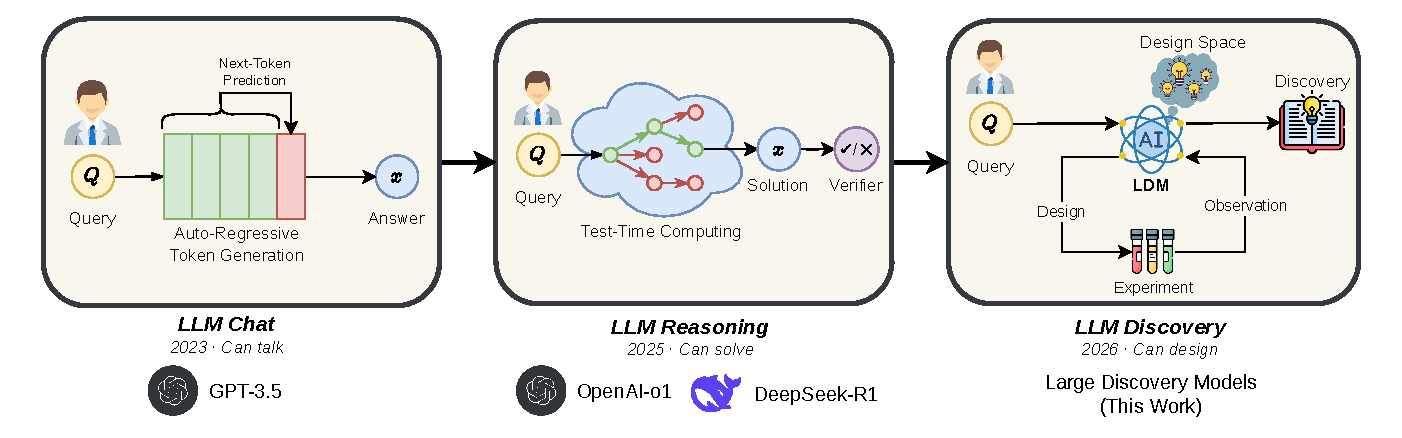
\includegraphics[width=\textwidth]{figure/evolution.drawio.pdf}
    \vspace{-20pt}
    \caption{
    \textbf{From generation and reasoning to open-ended discovery.}
    \emph{LLM generation} produces a response to a user query through
    autoregressive prediction \citep{brownLanguageModelsAre2020}.
    \emph{LLM reasoning} uses additional inference-time computation, such as
    chain-of-thought, tree search, or best-of-$N$ sampling, to generate,
    evaluate, and refine candidate solutions, typically with access to a cheap verifier \citep{openaiOpenAIO1System2024,wang2024openr,
    deepseek-aiDeepSeekR1IncentivizingReasoning2025}.
    \emph{Large Discovery Models} extend this loop to open-ended scientific
    design spaces, where evaluation requires costly interaction with the
    external world. Experimental observations update the model and guide the
    subsequent generation and selection of hypotheses or designs.
    }
    \label{fig:evolution}
\end{figure*}


\section{Introduction}
\label{sec:intro}

The development of large language models (LLMs) has progressed from
open-ended generation towards increasingly capable forms of reasoning.
Pretraining provides broad linguistic and conceptual knowledge, while
inference-time scaling allows a model to generate, compare, and refine
multiple candidate solutions. This approach has produced substantial gains in
mathematics, coding, theorem proving, and game playing, where solutions may be
difficult to find but comparatively easy to evaluate. Formal derivations can
be assessed by process or outcome verifiers, programs can be executed against
unit tests, and game strategies can be evaluated using exact rules or
simulators
\citep{yao2023tree,madaan2023selfrefine,snell2025scaling}.
AlphaZero-like methods make this feedback loop explicit by combining
generation, evaluation, and search
\citep{silver2017mastering,fengAlphazerolikeTreeSearchCan2024}.
OpenR~\citep{wang2024openr} provides an open framework for studying such
reasoning systems, while AlphaEvolve~\citep{novikov2025alphaevolve} couples
language-model proposals with automated evaluators at scale. Together, these
developments demonstrate that inference-time computation is particularly
effective when reliable and repeatable feedback can turn generation into
directed search.

Scientific discovery poses a more challenging setting. The candidate space may be vast, structured, and only partially specified, while feedback often depends on expensive simulation, accelerator experiments, physical assays, or real-world experiment. Evaluations cannot be repeated freely, and the resulting feedback may be delayed or noisy. A discovery system must therefore decide not only which candidates to evaluate, but also which hypotheses and designs should enter the search process in the first place. Figure~\ref{fig:evolution} illustrates this progression from generation and reasoning to discovery.



\begin{definition}[Scientific discovery]
\label{def:scientific-discovery}
Scientific discovery, in the setting considered here, is a sequential process
in which an agent generates hypotheses or designs, selects a limited number
for evaluation through interaction with an external evaluator, and uses the
resulting empirical observations to update its beliefs and guide subsequent
search. A discovery occurs when this
process identifies a previously unknown and non-trivial relationship,
mechanism, or design that is supported by empirical evidence.\footnote{This is an operational definition of empirically grounded,
search-based scientific discovery: the class of scientific problems that can
be formulated as sequential search over hypotheses or designs, with selected
candidates evaluated through physical experiments, simulations, computational
tests, or other external sources of evidence. It does not encompass all forms
of scientific discovery, particularly those for which the relevant search
space, evaluation procedure, or objective cannot yet be specified. Moreover,
\emph{unknown} and \emph{non-trivial} are relational notions, defined relative
to the agent's prior knowledge and, where appropriate, the knowledge of the
relevant scientific community. A result may therefore be a discovery for an
agent while constituting a rediscovery from the community's perspective.}
\end{definition}

\begin{figure*}[h]
    \centering
    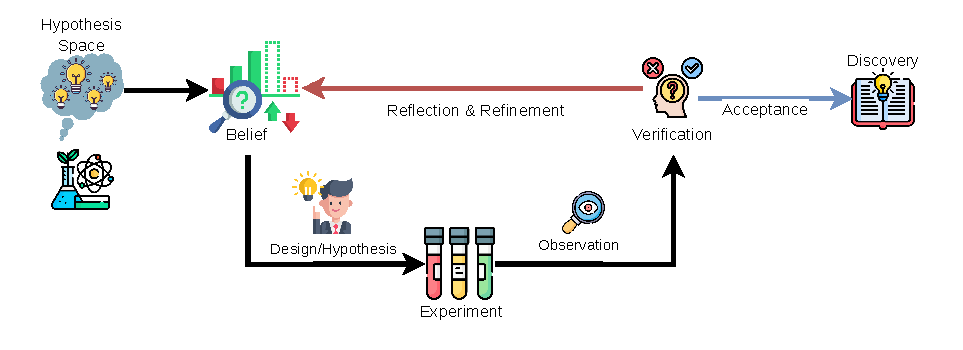
\includegraphics[width=\textwidth]
    {figure/discovery.drawio.pdf}
    \caption{
    \textbf{The Experimental Scientific Discovery (ESD) loop.}
    An agent generates candidate hypotheses or designs, selects a subset for
    costly evaluation, observes the outcomes, and uses those observations to
    update its beliefs and guide the next round of search, as described in
    Definition~\ref{def:scientific-discovery}.
    }
    \label{fig:scientific-discovery}
\end{figure*}

Definition~\ref{def:scientific-discovery} highlights two differences between
scientific discovery and reasoning with cheap verifiers. First, scientific
search is often \emph{open-ended}: relevant candidates may lie outside the
region represented by the current model or reachable through its existing
search operators. Second, empirical feedback is \emph{budgeted}: only a small
fraction of the generated candidates can be evaluated. The agent must
therefore learn from limited observations, model an unknown objective, and
allocate its experimental budget to candidates that are expected to be useful
or informative
\citep{shahriari2016taking,frazier2018tutorial}.

Current LLM-based research systems address only part of this problem.
Autonomous research agents can generate hypotheses, write code, execute
experiments, analyse results, and produce scientific manuscripts
\citep{lu2024aiscientist}. LLM-generated research proposals have also been
judged more novel than proposals written by human experts
\citep{si2024novelideas}. However, these proposals exhibit limited diversity
and weaker feasibility, and LLMs do not reliably evaluate their own ideas.
End-to-end assessments similarly identify persistent limitations in
experimental execution, novelty assessment, and methodological reasoning
\citep{beel2025aiscientist,xu2026researchclawbench,
starace2025paperbench}. Thus, fluent generation and procedural automation do
not by themselves provide the empirically grounded value signal needed for
scientific discovery.

This limitation also appears in scientific design. An LLM assigns high
probability to candidates that are plausible under its learned distribution,
but linguistic or sequence likelihood need not correlate with an externally
measured scientific property
\citep{guptaLLMsBayesianOptimization2025,chang2025llinbo}. LLM-only search can therefore produce
valid candidates without reliably determining which ones merit expensive
evaluation. Bayesian optimisation (BO) offers a complementary capability. Given a limited
set of observations, BO learns a probabilistic surrogate of the unknown
objective and uses an acquisition function to balance predicted performance
against epistemic uncertainty
\citep{jonesEfficientGlobalOptimization1998,srinivas2010gaussian,shahriari2016taking,
frazier2018tutorial}. It can therefore prioritise promising or informative
experiments under a limited evaluation budget. However, BO still requires a
representation of the design space and a mechanism for proposing or reaching
candidates. In structured and combinatorial spaces, such as molecules,
proteins, programs, and experimental protocols, optimising the acquisition
function may itself be difficult
\citep{balandat2020botorch,griffiths2020constrained}. BO can efficiently rank
the candidates exposed by its current representation and search operators,
but it may fail to reveal valuable candidates outside that search support.

These observations expose complementary limitations. LLMs can generate and
modify structured candidates, but lack a reliable estimate of their external
scientific value. BO grounds candidate selection in empirical observations,
but its effectiveness depends on which candidates its representation and
search procedure can expose. Scientific discovery requires both capabilities:
the search frontier must expand, and experimental resources must be allocated
using an uncertainty-aware value signal that balances expected value with information gain.
\begin{figure*}[t!]
    \centering
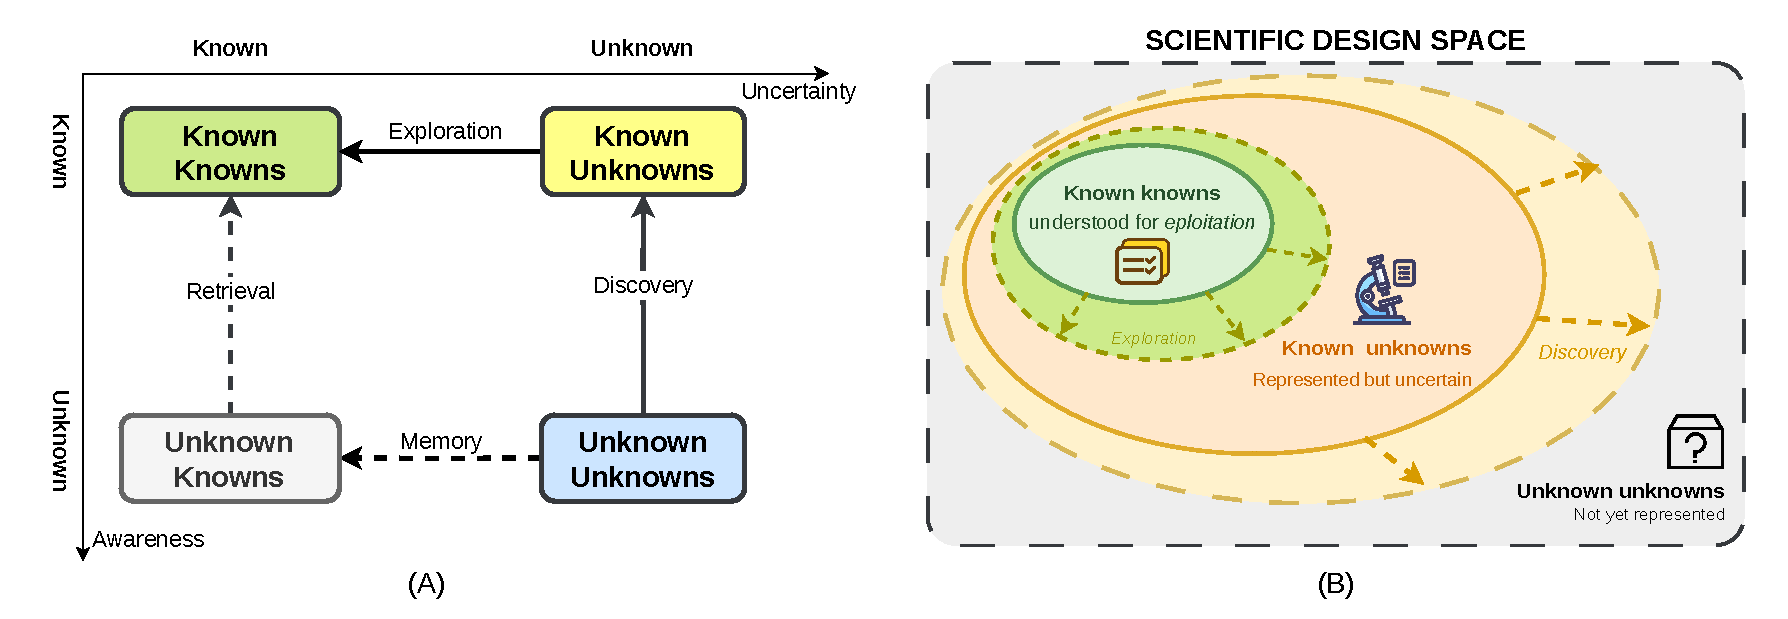
\includegraphics[width=\textwidth]
{figure/scientific_discovery_knowledge_map.drawio.pdf}
    \caption{
    \textbf{Epistemic regimes of experimental scientific search.}
    \textbf{(A)} An adaptation of the Rumsfeld Matrix
\citep{krogerus2018decision}, organised by search awareness and objective
    uncertainty.
    \textbf{(B)} A scientific agent moves among three regimes in the design
    space. 
    %\emph{Discovery} exposes previously unrepresented possibilities and turns them into explicit candidates or research questions. \emph{Exploration} reduces uncertainty about represented candidates and converts them into validated knowledge. \emph{Exploitation} uses this knowledge to select, verify, or deploy promising designs. Unknown knowns, which concern knowledge that is available but not explicitly represented, are outside the scope of this work and are omitted from Panel~B.
    }
    \label{fig:knowledge-regimes}
\end{figure*}

We formalise this problem as \emph{sequential inverse design}. A forward model
predicts the properties of a given design, whereas inverse design asks which
candidate should be evaluated next to achieve a desired property or maximise
an unknown reward. Evaluations may involve physical measurements, simulations,
computational tests, or other external sources of evidence. Because these
evaluations can be costly, only a limited number of candidates can be examined.
At the same time, the structured design space may be combinatorial, effectively
unbounded, or impossible to enumerate. Accurately modelling the reward across
the entire design space is therefore infeasible.

Instead, the agent maintains a \emph{probabilistic surrogate}: a data-efficient
model of the unknown reward learned from the candidates evaluated so far. For
each candidate within its modelling support, the surrogate provides both a
predicted reward and an estimate of \emph{epistemic uncertainty}. Epistemic
uncertainty reflects limitations in the surrogate's knowledge arising from
insufficient or uninformative observations. It can therefore be reduced by
collecting relevant new evidence. This differs from irreducible randomness or
measurement noise in the evaluation itself. After each evaluation, the new
observation is incorporated into the surrogate, updating both its predictions
and its uncertainty.

An \emph{acquisition function} converts the surrogate's predictions and
uncertainties into a measure of how useful it would be to evaluate or further
develop each candidate. It balances candidates predicted to perform well
against candidates that remain uncertain but potentially valuable. An
acquisition value is therefore not simply a predicted reward; it represents
the candidate's value to the sequential search process. The agent uses this
signal to allocate limited inference-time computation and to select candidates
for costly empirical evaluation. It consequently alternates among candidate
generation, evaluation selection, and belief updating.

This formulation separates two epistemic dimensions. The first is
\emph{predictive uncertainty}: how uncertain the surrogate is about the reward
of a candidate represented within its current modelling support. The second is
\emph{search awareness}: whether a candidate is represented by, or reachable
through, the current proposal and search process. Together, these dimensions
distinguish three modes of scientific search:

\begin{itemize}
    \item \emph{Exploitation} selects reachable candidates that the surrogate
    predicts will perform well.

    \item \emph{Exploration} evaluates reachable candidates about which the
    surrogate has high epistemic uncertainty, thereby improving knowledge
    within the current search support.

    \item \emph{Discovery} expands or reshapes the search support to reveal
    candidates, design families, or relationships that were not previously
    represented or reachable.
\end{itemize}

Figure~\ref{fig:knowledge-regimes} illustrates this perspective by adapting
the four epistemic regimes to scientific design. It distinguishes uncertainty
about candidates within the current search support from a lack of awareness of
candidates outside that support. Exploration reduces uncertainty about what is
already represented, whereas discovery changes what can be represented and
reached.

Motivated by this distinction, we introduce the \emph{Large Discovery Model}
(LDM), an empirically grounded recurrent architecture that couples an LLM
proposal model with a continually updated probabilistic surrogate. The LLM
generates, edits, and refines structured candidates, thereby constructing a
dynamic search frontier. The surrogate estimates the candidates' rewards and
quantifies its epistemic uncertainty about them. The acquisition function uses
these estimates to determine which candidates merit further refinement,
additional inference-time computation, or costly empirical evaluation. Each
new observation updates the surrogate and, through the acquisition signal,
redirects subsequent generation and search.

The acquisition function is therefore more than a post-generation filter. It
provides an empirically grounded value signal for allocating both computational
and evaluation resources. The LLM expands and reshapes the set of reachable
candidates, while the surrogate and acquisition function guide search over
this evolving set. In this way, LDM extends inference-time scaling from tasks
with cheap and repeatable verifiers to scientific-design problems
characterised by costly, noisy, and limited empirical feedback.
\begin{figure*}[t]
    \centering
    \begin{subfigure}[t]{0.42\textwidth}
        \centering
        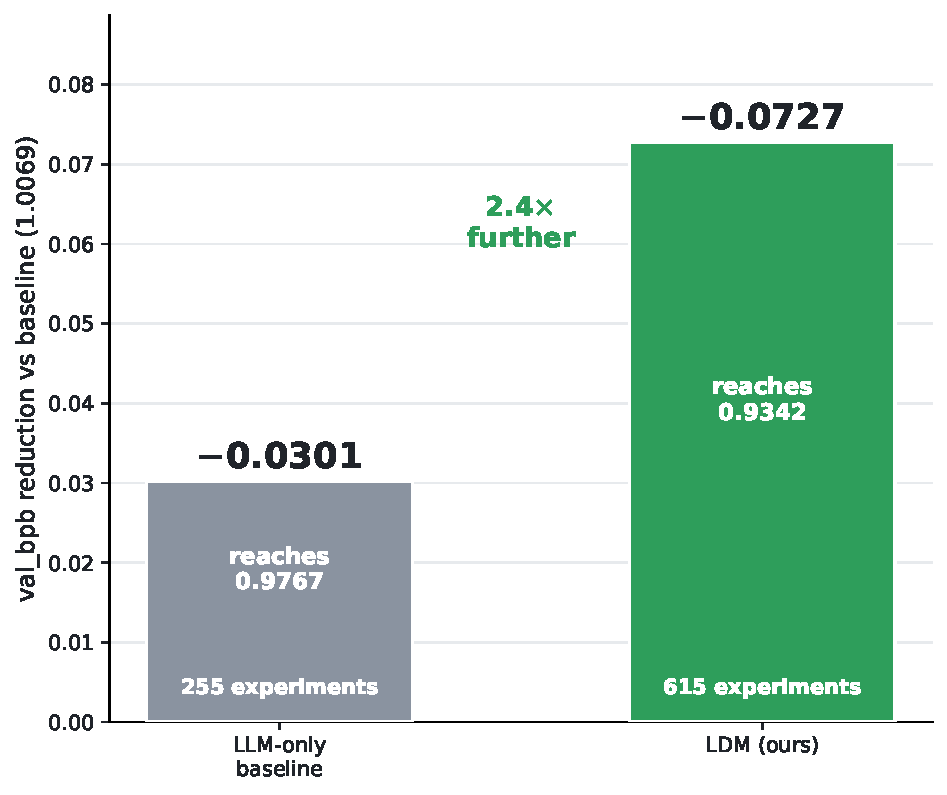
\includegraphics[width=\linewidth]
        {figure/improvement_two_bar.pdf}
        \caption{Performance on AutoResearch.}
        \label{fig:discovery-motivation-autoresearch}
    \end{subfigure}
    \hfill
    \begin{subfigure}[t]{0.42\textwidth}
        \centering
        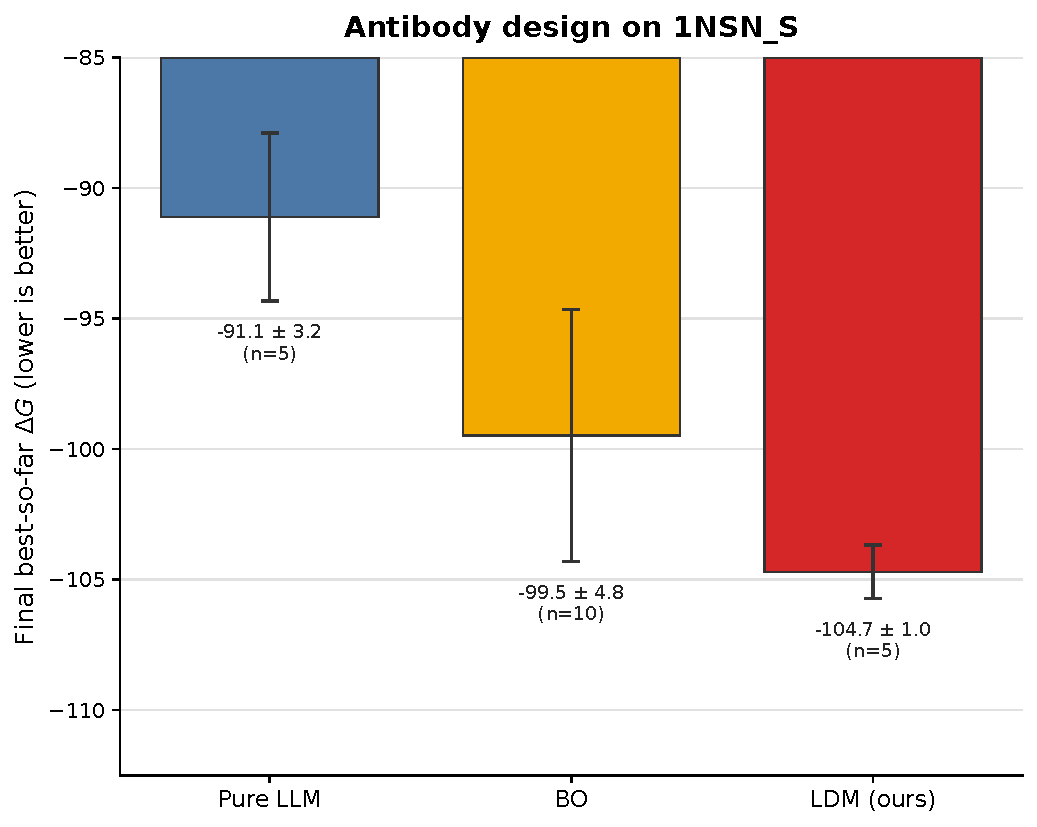
\includegraphics[width=\linewidth]
        {figure/discovery_motivation_antibody_1NSN_S.pdf}
        \caption{Performance on antibody design.}
        \label{fig:discovery-motivation-antibody}
    \end{subfigure}
    \caption{
    \textbf{Complementary limitations of LLM-only and BO-based search.}
    \textbf{(a)} LDM improves upon the LLM-only AutoResearch baseline under
    the same H100 hardware setting.
    \textbf{(b)} Final best-so-far binding energy on the antibody-design task,
    where LDM outperforms the LLM-only and BO-only baselines. Lower binding
    energy is better. For details, we refer to \S~\ref{sec:eval}.
    }
    \label{fig:discovery-motivation}
\end{figure*}


We evaluate LDM in three structured scientific-design domains:
neural-network training-program search on AutoResearch
\citep{karpathy2026autoresearch}, antibody CDRH3 sequence design, and
multi-objective molecular optimisation. LDM exceeds the best previously
reported AutoResearch result. With a weak language-model prior, it remains
competitive with AntBO~\citep{khan2022antbo}, a specialised BO method for
antibody design. It also achieves substantial improvements over both LLM-only
and BO-only baselines in multi-objective molecular design. Figure~\ref{fig:discovery-motivation} presents selected
results, with the full experimental evaluation deferred to
\S~\ref{sec:eval}.

Our contributions are fourfold. First, we formulate scientific discovery as
inference-time search over a dynamic, structured design space, guided by an
uncertainty-aware value model grounded in empirical observations. Second, we
introduce an acquisition-tilted search policy that combines the structured
prior of an LLM with inference-time computation and sequential experimental
feedback. Third, we provide a regret analysis that separates surrogate-model
error from the suboptimality of the LLM-based search process. Finally, we
demonstrate the framework across three classes of scientific objects:
computer programs, biological sequences, and molecules.


The remainder of the paper is organised as follows.
\S~\ref{sec:ldm} introduces the idea of discovery and its epistemic regimes.
\S~\ref{sec:method} derives the LDM formulation and its acquisition-tilted search method. \S~\ref{sec:algo} presents the practical algorithm.
\S~\ref{sec:theory-main} provides the regret analysis.
Finally, \S~\ref{sec:eval} reports the empirical results.


% ============================================================
\section{Search and Discovery in Open-Ended Design Spaces}
\label{sec:ldm}
% ============================================================

In this work, we aim to discover a design or hypothesis $x\in\X$ that achieves the highest
reward $R(x)$, i.e.\ to find or closely approximate
$x^\star\in\argmax_{x\in\X}R(x)$. This setting presents two intrinsic
difficulties. First, $R$ is a black-box function that is expensive to evaluate
and potentially noisy. Second, the hypothesis space $\X$ is typically open-ended: vast,
combinatorial, structured, or not even fully specified in advance, as in the
design of molecules, biological sequences, computer programs, and experimental
workflows.

This differs from classical numerical optimisation or combinatorial search,
which generally assumes a fixed and explicitly specified domain together with
a gradient, numerical oracle, or known set of valid search operations. In
scientific discovery, the full hypothesis space may not be enumerable, and the
search may need to formulate hypotheses that lie beyond its current
representation or reach.

To reason about what is currently known, we introduce
\emph{a probabilistic surrogate}, i.e.\ a posterior
$p(R\mid\mathcal{D}_t)$ over the reward surface $R$ conditioned on the dataset
$\mathcal{D}_t=\{(x_i,r_i)\}_{i=1}^{t-1}$ of previously evaluated designs and
their noisy feedback $r_i\approx R(x_i)$. Its predictive belief is usually
summarised by posterior moments $(\mu_t(x),\sigma_t(x))$, representing the
expected reward and predictive uncertainty on the surrogate's modelling
support. The surrogate therefore describes the search's current empirical
knowledge, but it does not by itself determine or enumerate the full
hypothesis space.

Using this surrogate-relative notion of knowledge, we partition $\X$ into four
epistemic regimes, as illustrated in
Figure~\ref{fig:knowledge-regimes}.

\begin{itemize}[leftmargin=1.6em,itemsep=2pt,topsep=2pt]
    \item \emph{Known knowns} are evaluated designs whose rewards are
    sufficiently well understood. The surrogate predicts their values with
    low posterior uncertainty $\sigma_t(x)$.

    \item \emph{Known unknowns} are designs that the search can formulate and
    the surrogate can model, but whose rewards remain unresolved. They are
    represented by high posterior uncertainty $\sigma_t(x)$ and can be
    resolved through further evaluation.

\item \emph{Unknown knowns} are designs or evaluation results that exist in
    an external source, such as a database, a previous experiment, or a
    parallel discovery process, but are absent from the current search
    context. They can become available only through an explicit retrieval
    operation.
    
    \item \emph{Unknown unknowns} are designs that lie beyond the search's
    current effective reach. This can occur for two reasons:
    (i)~$\X$ is too large, combinatorial, or effectively unbounded for the current
    search procedure to reach the design; or (ii)~the design lies outside the
    surrogate's modelling support, so that $(\mu_t(x),\sigma_t(x))$ does not
    constitute a meaningful calibrated prediction.
\end{itemize}

These regimes distinguish uncertainty, reachability, modelling, and
knowledge. A design does not become known merely because it belongs to a
mathematically defined space; a reachable design is not necessarily supported
by the surrogate; and information stored externally is not available unless
it is retrieved into the current context. All four regimes may therefore
persist throughout the search.

The \emph{search frontier} is the conceptual boundary of what the current
procedure can effectively formulate, reach, and model. Designs inside this
frontier are accessible to the search, although their rewards may remain
uncertain. Designs outside it have not yet entered the modelled search
process. This distinction gives rise to three operations closely related to \cite{wang2008infinitely}:

\begin{itemize}[leftmargin=1.6em,itemsep=2pt,topsep=2pt]
    \item \emph{Exploitation} acts on known knowns by selecting designs for
    which the surrogate predicts both high reward $\mu_t(x)$ and low
    uncertainty $\sigma_t(x)$.

    \item \emph{Exploration} resolves known unknowns by evaluating reachable
    but uncertain designs. The resulting observations reduce posterior
    uncertainty and may turn known unknowns into known knowns.

    \item \emph{Discovery} expands the search frontier by formulating
    hypotheses that were previously outside the search's effective reach.
    This brings unknown unknowns into the modelled hypothesis space, where they
    become known unknowns that can subsequently be evaluated.
\end{itemize}

Discovery is therefore not simply the evaluation of an untested design. An
untested design that already lies within the surrogate's modelling support is
a known unknown and belongs to exploration. Discovery instead changes what
the search can express, reach, or meaningfully model. Experimental evaluation
then determines the value of the newly surfaced hypothesis.

The three operations correspond to three transitions in
Figure~\ref{fig:knowledge-regimes}: discovery moves hypotheses from unknown
unknowns to known unknowns, exploration moves them from known unknowns to
known knowns, and exploitation operates within the known-known regime. The
unknown-known regime requires separate memory read and write operations. We
leave memory retrieval and federated discovery to future work and focus here
on discovery, exploration, and exploitation within a single sequential search
process.

This formulation is conceptual and does not prescribe a particular discovery
algorithm. The next section introduces the Large Discovery Model, which
instantiates these operations by combining a generative foundation model, the
probabilistic surrogate introduced above, and an acquisition-guided
inference-time search policy.



% ============================================================
\section{The Large Discovery Model}
\label{sec:method}
% ============================================================

We are now ready to define the \emph{Large Discovery Model} (LDM). LDM is a
policy for sequential inverse design built from three interacting components:
a generative foundation model, a probabilistic surrogate, and a model-based
acquisition function.

Same as before at iteration $t$, let
\[
\mathcal{D}_t=\{(x_i,r_i)\}_{i=1}^{t-1}
\]
denote the empirical evaluation history, where $x_i$ is a previously evaluated
design and $r_i$ is its observed reward. We use $\mathcal{C}_t$ to denote the
broader \emph{search context} available to the generative model. This context
may include $\mathcal{D}_t$, previously generated candidates, surrogate
predictions, acquisition values, constraint feedback, refinement trajectories,
and other forms of search memory. Thus, $\mathcal{D}_t$ contains the empirical
evidence used to fit the surrogate, whereas $\mathcal{C}_t$ contains the
information used to condition candidate generation.

\paragraph{(i) A generative foundation model.}
We denote by
\begin{equation}
    p_{\theta,\alpha}(x\mid\mathcal{C}_t)
\end{equation}
the proposal distribution over plausible designs conditioned on the current
search context. Here, $\theta$ denotes the parameters of the underlying
generative model, while $\alpha$ denotes its inference configuration, such as
the prompting strategy, sampling temperature, reasoning procedure, refinement
scheme, or inference-time compute budget. We use $p_{\theta,\alpha}$ throughout
the paper to make explicit that the effective proposal distribution depends
not only on the model parameters but also on how the model is used at
inference time.

The generative model supplies a structured prior over the design space
$\mathcal{X}$. It enables the search to generate candidates that reflect
domain knowledge, semantic plausibility, and structural constraints without
requiring $\mathcal{X}$ to be explicitly enumerated. By changing its context
or inference procedure, the model can also expand and reshape the set of
candidates reachable by the current search.

\paragraph{(ii) A probabilistic surrogate.}
As introduced in Section~\ref{sec:ldm}, the posterior
\[
    p(R\mid\mathcal{D}_t)
\]
represents the current belief about the unknown reward function, conditioned
on the empirical observations collected so far. For a candidate $x$, the
predictive mean $\mu_t(x)$ estimates its expected reward, while the predictive
uncertainty $\sigma_t(x)$ quantifies the surrogate's epistemic uncertainty
about that estimate. High epistemic uncertainty indicates that the prediction
is weakly supported by the available evidence and may be reduced through
additional informative evaluations. It is therefore distinct from
irreducible randomness or measurement noise in the evaluation process.

The surrogate provides the empirical grounding that the generative model
alone generally lacks. Although a foundation model may encode substantial
domain knowledge, its likelihoods and self-assessments do not necessarily
provide calibrated estimates of a task-specific quantitative reward,
particularly for novel candidates outside the observed data distribution.

\paragraph{(iii) A model-based acquisition function.}
From the surrogate's predictive distribution, we construct an acquisition
function
\[
    \acq_t(x)
\]
that assigns each candidate a scalar value to the sequential search process.
Depending on its form, the acquisition function may favour candidates with
high predicted reward, candidates with high epistemic uncertainty, or a
principled combination of the two. It therefore mediates the trade-off between
exploitation and exploration.

The acquisition value should not be interpreted simply as the predicted
reward of a candidate. Rather, it measures the potential value of allocating
further computation or empirical evaluation to that candidate. It can be used
both to decide which candidates warrant costly external evaluation and to
direct inference-time operations such as sampling, ranking, refinement, and
branch expansion.

These three components play complementary roles. The generative model proposes
structured candidates and can move the search frontier towards designs not
previously considered. The surrogate grounds the search in empirical
observations and quantifies epistemic uncertainty. The acquisition function
uses this predictive belief to determine which reachable candidates are most
valuable to develop or evaluate. LDM thereby uses empirically calibrated
feedback to direct the inference-time search of the generative model.

%\subsection{Acquisition-Tilted Search}

We seek a search distribution that attains high expected acquisition value
while remaining sufficiently close to the structured prior supplied by the
generative model. Assume that $\mathcal{X}$ is a measurable space, with its
$\sigma$-algebra omitted for simplicity. At iteration $t$, we define
\begin{equation}
\label{eq:variational}
    \pi_t
    =
    \argmax_{q\in\Delta(\mathcal{X})}
    \left\{
        \mathbb{E}_{x\sim q}\!\left[\acq_t(x)\right]
        -
        \frac{1}{\eta}
        \KL\!\left(
            q
            \,\middle\|\,
            p_{\theta,\alpha}(\cdot\mid\mathcal{C}_t)
        \right)
    \right\},
\end{equation}
where $\Delta(\mathcal{X})$ denotes the set of probability measures over
$\mathcal{X}$, $\KL$ is the Kullback--Leibler divergence, and $\eta>0$ controls
the strength of acquisition-based tilting. The expected-acquisition term moves
probability mass towards candidates that are valuable under the empirically
grounded surrogate. The KL term prevents the search policy from departing
arbitrarily far from the generative model's prior over plausible and
well-formed designs. The parameter $\eta$ controls this trade-off: larger
values place greater emphasis on acquisition value, whereas smaller values
keep the search closer to the generative prior.

The inference configuration $\alpha$ affects $\pi_t$ through
$p_{\theta,\alpha}(\cdot\mid\mathcal{C}_t)$ and therefore changes the reference
distribution against which the KL divergence is measured. Increasing
inference-time computation may reshape this proposal distribution through
additional sampling, reasoning, refinement, or structured search. The
acquisition function then determines how that computation is allocated
according to predicted empirical value and epistemic uncertainty.

Equation~\eqref{eq:variational} is deliberately model-agnostic: it does not
depend on a particular generative architecture, probabilistic surrogate, or
acquisition function. Its variational form follows the Gibbs variational principle and is closely
related to Gibbs posteriors~\citep{donsker1975variational,bissiri2016general},
KL-regularised policy search~\citep{peters2010relative},
maximum-entropy reinforcement learning~\citep{haarnoja2018soft}, and control as
probabilistic inference~\citep{levine2018reinforcement}. Accordingly, our contribution is not the generic
KL-regularised objective in isolation. The distinctive role of
Equation~\eqref{eq:variational} in LDM is to connect a structured generative
prior to an acquisition value derived from a continually updated empirical
surrogate. This connection allows external observations to direct both
inference-time computation and sequential evaluation over structured,
potentially open-ended design spaces.

The resulting policy is recurrent (see Fig~\ref{fig:loop}). Candidates generated under the current
search context are scored and refined using the surrogate-derived acquisition
signal; selected candidates are then evaluated by an external empirical
source; and the resulting observations update $\mathcal{D}_t$, the surrogate,
and the next search context $\mathcal{C}_{t+1}$. LDM therefore does not merely
reweight a fixed set of generated samples. It repeatedly couples generation,
empirical evaluation, belief updating, and search-frontier expansion.

In the following sections, we first show that
Equation~\eqref{eq:variational} admits a closed-form acquisition-tilted policy.
We then describe how this ideal policy can be approximated through
inference-time sampling, selection, and iterative refinement, with particular
attention to test-time compute scaling. We subsequently instantiate the
probabilistic surrogate as a Gaussian process and construct $\acq_t$ from its
posterior predictive distribution. Finally, we describe how the same
acquisition signal can support parameter adaptation: in addition to directing
inference through $\alpha$, it may provide supervision for updating the
generative parameters $\theta$ through fine-tuning.


\subsection{An Acquisition-Tilted Search Distribution}
\label{sec:core}

With the LLM prior $p_{\theta,\alpha}$ and the acquisition function $\acq_t$ defined, our desired search policy $\pi_t$ follows directly from the variational objective in Eq.~\eqref{eq:variational}. This variational problem is a canonical instance of the Gibbs variational principle (equivalently, the Donsker–Varadhan representation of the KL divergence)~\citep{donsker1975variational,bissiri2016general}, whose unique maximiser is the exponentially tilted distribution. This form of KL-regularised reward maximisation is the same mathematical foundation underlying maximum-entropy reinforcement learning, control-as-inference \citep{levine2018reinforcement}, and the closed-form policy objective in KL-regularised RLHF \citep{rafailov2023direct}.

\begin{proposition}[Optimal search distribution]
\label{prop:gibbs}
The unique maximiser of \eqref{eq:variational} is
\begin{equation}
\label{eq:core}
\pi_t(x)=\frac{1}{Z_t}\,p_{\theta,\alpha}(x\mid\mathcal{C}_t)\,\exp\!\big\{\eta\,\acq_t(x)\big\},
\qquad Z_t=\int_{x\in\mathcal{X}}p_{\theta,\alpha}(x\mid\mathcal{C}_t)\,\exp\!\big\{\eta\,\acq_t(x)\big\}\,\mathrm{d}x.
\end{equation}
\end{proposition}
\begin{proof}
Please refer to Appendix~\ref{prop_proof}.
\end{proof}

Eq.~\eqref{eq:core} shows that the optimal policy $\pi_t$ takes an acquisition-tilted form, where the base measure is reweighted by the exponent of the acquisition function. Interestingly, this policy draws an analogy to the infinite-armed bandit framework \citep{berry1997bandit,wang2008infinitely}: as scientific designs (arms) cannot be listed in advance, they are revealed from a reservoir distribution, and the policy tilts that reservoir toward arms it judges valuable. In this reading, $p_{\theta,\alpha}(\cdot\mid\mathcal{C}_t)$ plays the role of the reservoir, $\eta\,\acq_t(x)$ acts as the strength-of-reward tilt, and $Z_t$ is the usual log-sum-exp normaliser.

A clear interpretation of the inference configuration $\alpha$ and the KL-regularisation coefficient $\eta$ can be drawn through standard analysis of infinite-armed bandits. We restrict attention to the common case in which the reservoir admits the temperature form
\begin{equation}
  \label{eq:temp}
  p_{\theta,\alpha}(x\mid\mathcal{C}_t) \propto p_\theta(x\mid\mathcal{C}_t)^\alpha,
\end{equation}
where $p_\theta$ denotes the unconditional base proposal. This is the exponential family of reservoirs commonly used in the bandit literature, and it makes $\alpha$ transparent as the strength of the prior: large values of $\alpha$ concentrate probability mass on modes of $p_\theta$, while $\alpha\to 0$ spreads mass toward a uniform measure on $\mathcal{X}$. Substituting this form into \eqref{eq:core} and taking the mode gives the bandit-style argmax
\begin{equation}
  \label{eq:argmax}
  x_{t+1}=\argmax_{x\in\mathcal{X}}\ \Big[\ \alpha\,\log p_\theta(x\mid\mathcal{C}_t)+\eta\,\acq_t(x)\ \Big],
\end{equation}
which picks the arm that maximises a weighted combination of the prior log-mass $\log p_\theta$ and the reward tilt $\acq_t$, i.e., the bandit analogue of selecting the most promising revealed arm.

Examining the two limiting cases of the temperature form $p_{\theta,\alpha}(x\mid\mathcal{C}_t)\propto p_\theta(x\mid\mathcal{C}_t)^\alpha$ situates LDM relative to related paradigms. As $\eta\to 0$ the tilt vanishes and $\pi_t$ collapses to the raw reservoir $p_{\theta,\alpha}(\cdot\mid\mathcal{C}_t)$, so search is driven entirely by the generative model with no data feedback. As $\alpha\to0$ the reservoir spreads toward a uniform measure on $\mathcal{X}$ and the policy becomes $\pi_t\propto\exp\{\eta\,\acq_t(\cdot)\}$, recovering classical Bayesian optimisation once $\eta$ is also taken large. LDM is the regime between these two limit points, where both the structured prior and the uncertainty-aware acquisition contribute to the policy. We note, however, that some LLM inference backends do not admit the temperature form $p_\theta(x\mid\mathcal{C}_t)^\alpha$, and the preceding analysis should be read as the canonical case under which the role of $\alpha$ is most cleanly interpreted.

With this construction, LDM defines a discovery policy $\pi_t$ from which new designs may be drawn using either a stochastic or a deterministic approach, as illustrated by Eq.~\eqref{eq:argmax}. In practice, the normalising constant $Z_t$ is never computed explicitly, and we instead rely on inference-time search to approximate draws from the tilted distribution.

\subsection{Surrogate Modelling of the Reward Function}
\label{sec:surrogate}

To efficiently navigate the design space, we require a probabilistic model over function space that treats the reward function $R$ as a random function and models the posterior belief $R \mid \mathcal{D}_t$ conditioned on our cumulative evaluations. Our LDM formulation is largely inspired by the uncertainty-aware decision-making paradigm of Bayesian optimisation \citep{garnettBayesianOptimization2023}.

We model this objective using a Gaussian Process (GP) \citep{rasmussen2006gaussian}. GPs serve as highly effective surrogates in this setting because they are exceptionally sample-efficient, admit exact Bayesian updates, and provide principled non-parametric uncertainty estimates across unexplored regions of the design space. Formally, we define the prior distribution over the reward function as:
\begin{equation}
\label{eq:gp_prior_main}
R(x) \sim \mathcal{GP}\bigl(m(x),\, k(x, x')\bigr),
\end{equation}
where $m: \mathcal{X} \to \mathbb{R}$ is the prior mean function and $k: \mathcal{X} \times \mathcal{X} \to \mathbb{R}$ is a positive-definite kernel function capturing spatial correlation. 

By conditioning this prior on the historical data $\mathcal{D}_t = \{(x_i, r_i)\}_{i=1}^{t}$, we obtain a Gaussian posterior distribution characterised by a predictive mean $\mu_t(x)$ and a predictive variance $\sigma_t^2(x)$ for any candidate point $x \in \mathcal{X}$. These two statistical moments allow us to construct acquisition functions that elegantly balance exploitation (seeking high predicted rewards) and exploration (targeting regions of high uncertainty). For instance, the popular Upper Confidence Bound (UCB) acquisition function is formulated as:
\begin{equation}
\label{eq:ucb_main}
\alpha^{\mathrm{UCB}}_t(x) = \mu_t(x) + \sqrt{\beta_t}\,\sigma_t(x),
\end{equation}
where $\beta_t > 0$ is a parameter scaling the exploration incentive. The complete technical details of the posterior inference, along with the formulation of other common acquisition functions, are provided in Appendix~\ref{sec:llm-bo}.

Because UCB decomposes the decision value into a high-mean and a high-uncertainty term, the tilted policy $\pi_t(x)\propto p_{\theta,\alpha}(x\mid\C_t)\exp\{\eta\,\acq_t(x)\}$ of Eq.~\eqref{eq:core} instantiates the discovery--exploration--exploitation triangle of Figure~\ref{fig:knowledge-regimes} directly: the LLM reservoir term realises discovery, the high-$\sigma_t$ tail of $\acq_t$ realises exploration, and the high-$\mu_t$ mode realises exploitation. We use UCB as the running example precisely because the trade-off is explicit in its closed form; in richer acquisitions the same triangle is realised only implicitly through the surrogate.

\subsection{Acquisition-Tilted Inference-Time Search}
\label{sec:inference-time-search}

Exact evaluation or sampling of $\pi_t$ is computationally intractable over the high-dimensional, combinatorial design spaces typical of scientific discovery. We therefore approximate the tilted distribution via inference-time search: the LLM proposes a finite pool of candidates, which are then reweighted by the acquisition function to align with the target distribution. This framework naturally supports test-time compute scaling, mirroring the broader paradigm in general LLM reasoning but guided by a calibrated, task-grounded value signal rather than model-internal confidence~\citep{wang2024openr}.

We consider two canonical approximation schemes. The deterministic best-of-$N$ rule targets the mode of the tilted distribution: we draw $N$ independent candidates from the LLM prior,
\[
\{\hat{x}_{t,i}\}_{i=1}^N \sim p_{\theta, \alpha}(\cdot \mid \mathcal{C}_t),
\]
and select the candidate with the highest acquisition score:
\[
x_{t+1} = \argmax_{i \in \{1,\dots,N\}} \acq_t(\hat{x}_{t,i}).
\]
The proposal $p_{\theta,\alpha}$ may comprise a collection of hyperparameters, e.g.,\ temperature and top-$p$ for an autoregressive decoder, or a noise schedule for a diffusion sampler, depending on the backend. The single explicit tunable below is $\eta$; the rest of $p_{\theta,\alpha}$ is held fixed.

The stochastic scheme approximates sampling from the full tilted distribution via softmax reweighting, where sampling probability is proportional to the exponentiated acquisition value:
\begin{equation}
\label{eq:softmax_reweight}
\Pr(x_t = \hat{x}_{t,i})
=
\frac{\exp\bigl\{\eta \, \acq_t(\hat{x}_{t,i})\bigr\}}
{\sum_{j=1}^N \exp\bigl\{\eta \, \acq_t(\hat{x}_{t,j})\bigr\}}.
\end{equation}
For batch selection with $b>1$, these generalise naturally to top-$b$ selection for the deterministic case and Gumbel-top-$b$ sampling for the stochastic case.

Candidate pool size $N$ plays the critical role of \emph{test-time compute scaling}, a powerful technique for LLM reasoning \citep{wangTutorialLLMReasoning2025}, and LDM adapts this core advantage to discovery tasks. Larger $N$ improves the fidelity of the approximation to the optimal tilted distribution and lifts empirical performance, at the cost of additional LLM inference and surrogate evaluation. This aligns with the established finding that test-time compute can substitute for model scale in LLM reasoning, with the key distinction that LDM uses an externally calibrated acquisition function as guidance, rather than the model’s own self-evaluation or linguistic plausibility.

The full-candidate reweighting scheme is simple, modality-agnostic, and forms the basis of our experiments. For sequentially generated design spaces such as sequences and programs, the principle can be extended to intermediate generation steps via a prefix value function $V(x_{t,\le i}) = \mathbb{E}_{x_{t,>i}}[\acq_t(x_{t,\le i},x_{t,>i})]$, enabling more advanced methods such as beam search and Monte Carlo Tree Search~\citep{fengAlphazerolikeTreeSearchCan2024}. These multi-step variants offer further search coverage at higher computational cost, and we leave their full empirical evaluation as future work.

\begin{figure}[t]
\centering
\begingroup
\definecolor{llmred}{RGB}{249,220,220}%
\definecolor{llmredline}{RGB}{201,74,74}%
\definecolor{gpblue}{RGB}{214,231,247}%
\definecolor{gpblueline}{RGB}{58,110,165}%
\definecolor{graybox}{RGB}{238,238,238}%
\definecolor{grayline}{RGB}{120,120,120}%
\definecolor{fbgray}{RGB}{90,90,90}%
\resizebox{\textwidth}{!}{%
\begin{tikzpicture}[
    >={Latex[length=2.4mm]},
    font=\normalsize,
    llm/.style={draw=llmredline,line width=1pt,fill=llmred,rounded corners=5pt,
                align=center,inner sep=7pt,minimum height=20mm,text width=50mm},
    gp/.style={draw=gpblueline,line width=1pt,fill=gpblue,rounded corners=5pt,
                align=center,inner sep=7pt,minimum height=20mm,text width=50mm},
    proc/.style={draw=grayline,line width=0.9pt,fill=graybox,rounded corners=4pt,
                align=center,inner sep=6pt},
    lbl/.style={font=\small,align=center},
    fb/.style={font=\small\itshape,align=center,text=fbgray},
    flow/.style={->,line width=0.9pt},
    fbflow/.style={->,line width=1.0pt,fbgray},
]
 
% Top boxes
\node[llm] (llm) at (-2.9,3.7)
  {\textbf{LLM reservoir}\\[3pt]$p_{\theta,\alpha}(\cdot\mid\C_t)$};
\node[gp]  (gp)  at ( 2.9,3.7)
  {\textbf{GP surrogate: reward model}\\[3pt]$\mu_t,\sigma_t$, acquisition $\acq_t$};
 
% Tilted-search box
\node[proc,text width=78mm] (pi) at (0,0.65)
  {\textbf{acquisition-tilted search}\\[3pt]
   $\pi_t(x)\;\propto\;p_{\theta,\alpha}(x\mid\C_t)\,\exp\!\big\{\eta\,\acq_t(x)\big\}$};
 
% Candidate batch
\node[proc,text width=70mm] (cand) at (0,-1.65)
  {\textbf{draw candidate batch }$B_t=\{x_{t,1},\dots,x_{t,b}\}$};
 
% Evaluate batch
\node[proc,text width=68mm] (eval) at (0,-3.95)
  {\textbf{evaluate }$R(x)$\textbf{ for all }$x\in B_t$};
 
% Arrows: top boxes into pi
\draw[flow] (llm.south) -- (pi.north -| llm.south)
   node[lbl,midway,left=3pt] {base measure};
\draw[flow] (gp.south) -- (pi.north -| gp.south)
   node[lbl,midway,right=3pt] {acquisition function};
 
% pi -> cand -> eval
\draw[flow] (pi) -- (cand)
   node[lbl,midway,right=1pt] {inference-time search};
\draw[flow] (cand) -- (eval)
   node[lbl,midway,right=1pt] {query};
 
% Feedback loops (both labelled "feedback")
% eval -> llm  (update history)
\draw[fbflow] (eval.west) .. controls +(-3.6,0) and +(-1.8,0) .. (llm.west)
   node[fb,pos=0.28,fill=white,inner sep=2pt] {feedback}
   node[lbl,pos=0.62,fill=white,inner sep=2pt] {update history $\C_t$};
% eval -> gp  (update data)
\draw[fbflow] (eval.east) .. controls +(3.6,0) and +(1.8,0) .. (gp.east)
   node[fb,pos=0.28,fill=white,inner sep=2pt] {feedback}
   node[lbl,pos=0.62,fill=white,inner sep=2pt] {update data $\D_t$};
 
\end{tikzpicture}%
}
\endgroup
\caption{The Large Discovery Model loop. The LLM supplies the base measure
$p_{\theta,\alpha}(\cdot\mid\C_t)$ and the GP surrogate supplies the acquisition function
$\acq_t$; together they define the acquisition-tilted search distribution $\pi_t$. At each
round, inference-time search draws a candidate batch $B_t=\{x_{t,1},\dots,x_{t,b}\}$,
evaluates $R(x)$ for every $x\in B_t$, and feeds the observations back to update data $\D_t$
and history $\C_t$.}
\label{fig:loop}
\end{figure}


% ============================================================
\subsection{Fine-Tuning to Reduce Test-Time Search}
\label{sec:ldm-finetune}
% ============================================================

The LDM policy in Equation~\eqref{eq:core} combines the structured generative
prior (reservoir)
$p_{\theta,\alpha}(\cdot\mid\mathcal{C}_t)$
with the acquisition function $\acq_t$. A high-budget implementation of LDM
test-time search, denoted by LDM-TTS, approximates this policy by generating a
large pool of candidates and using the acquisition function to rank, select,
and refine the most valuable ones. Although effective, repeating this
procedure at every search round can require substantial inference-time
computation. We therefore propose to distil the behaviour of high-budget
LDM-TTS into a more efficient student proposer through fine-tuning.

At iteration $t$, the acquisition value of a candidate $x$ may be written
abstractly as
\begin{equation}
\label{eq:sft-acquisition}
    \acq_t(x)
    =
    \operatorname{Acq}\!\left(
        \mu_t(x),
        \sigma_t(x),
        g_t(x)
    \right),
\end{equation}
where $\mu_t(x)$ and $\sigma_t(x)$ are the surrogate's posterior predictive
mean and epistemic uncertainty, respectively. The term $g_t(x)$ collects
additional task-dependent considerations, such as constraint satisfaction,
novelty, evaluation cost, diversity, or expected improvement of the current
Pareto frontier.

Suppose that high-budget LDM-TTS generates a candidate pool
\[
    \widehat{\mathcal{X}}_t
    =
    \{\hat{x}_{t,i}\}_{i=1}^{N}
\]
under the search context $\mathcal{C}_t$. We define an acquisition-weighted
empirical distribution over this pool by
\begin{equation}
\label{eq:empirical-tilt}
    \widehat{\pi}_t(\hat{x}_{t,i}\mid\mathcal{C}_t)
    =
    \frac{
        \exp\!\left\{\eta\,\acq_t(\hat{x}_{t,i})\right\}
    }{
        \sum_{j=1}^{N}
        \exp\!\left\{\eta\,\acq_t(\hat{x}_{t,j})\right\}
    },
\end{equation}
where $\eta>0$ controls how strongly the distribution concentrates on
candidates with high acquisition values. This finite-pool distribution
approximates the ideal acquisition-tilted policy in
Equation~\eqref{eq:core}.

Let $p_{\phi}(x\mid\mathcal{C}_t)$ denote the student proposer, initialised
from the underlying generative model. We fine-tune it by minimising the
acquisition-weighted negative log-likelihood
\begin{equation}
\label{eq:acquisition-distillation}
    \mathcal{L}_{\mathrm{distill}}(\phi)
    =
    -
    \sum_t
    \sum_{i=1}^{N}
    \widehat{\pi}_t(\hat{x}_{t,i}\mid\mathcal{C}_t)
    \log p_{\phi}(\hat{x}_{t,i}\mid\mathcal{C}_t).
\end{equation}
Equivalently, this objective projects the finite-pool teacher policy
$\widehat{\pi}_t$ onto the family of distributions represented by the student
model. The resulting proposer assigns greater probability to candidates that
high-budget LDM-TTS would regard as valuable, allowing some of the benefits of
test-time search to be transferred into the model parameters.

Importantly, the training signal is richer than the single candidate
eventually selected for costly empirical evaluation. The unselected candidates
record which alternatives the generative model considered and how the
surrogate ranked their exploitation, exploration, and discovery value under
the same search context. Fine-tuning on this information amortises part of the
high-budget search process: the student learns to propose stronger candidates
directly and can therefore achieve comparable search quality with a smaller
candidate pool or fewer refinement steps at test time.

Because the surrogate and acquisition function change as new empirical
observations are collected, the distilled policy is associated with the
search states on which it was trained. It may therefore be updated
periodically as the empirical dataset and search frontier evolve, rather than
being treated as a permanently fixed replacement for online LDM search.
% Insert the existing Figure~\ref{fig:training-pipeline} TikZ block here.
% Keep its label and use the following concise caption.
%
% \caption{
% \textbf{Amortizing LDM test-time search.}
% High-budget LDM-TTS samples a candidate pool from the LLM reservoir and scores
% it with the current surrogate acquisition function. High-value search traces,
% optionally paired with surrogate-grounded rationales, are distilled through
% supervised fine-tuning into a low-budget discovery proposer.
% }
% \label{fig:training-pipeline}

\paragraph{Reasoning augmentation.}
Acquisition values rank candidates but do not explicitly state why a candidate
is useful for research progress. We therefore optionally augment selected
teacher traces with a short rationale
\begin{equation}
z_{t,i}
=
\operatorname{Explain}\Big(
\C_t,\hat{x}_{t,i},
\mu_t(\hat{x}_{t,i}),
\sigma_t(\hat{x}_{t,i}),
g_t(\hat{x}_{t,i}),
\acq_t(\hat{x}_{t,i})
\Big).
\label{eq:reasoning-augmentation}
\end{equation}
The rationale is grounded in the surrogate value decomposition. It can explain
whether a candidate exploits high predicted utility, probes an uncertain
region, satisfies a constraint, preserves diversity, or tests a new candidate
family after search stagnation. Thus, unlike reasoning traces for closed-world
problems, discovery rationales explain why a scarce experiment is worth
running.

We construct an SFT dataset of tuples
$(\C_t,z_{t,i},\hat{x}_{t,i})$, retaining or sampling candidate traces
according to $\widehat{\pi}^{(N)}_t$. Let $\bar{w}_{t,i}$ be normalized weights
derived from Eq.~\eqref{eq:empirical-tilt}. A student model $p_\phi$ is trained
with the weighted autoregressive objective
\begin{equation}
\mathcal{L}_{\mathrm{SFT}}(\phi)
=
-
\sum_t\sum_{i=1}^{N}
\bar{w}_{t,i}
\left[
\log p_\phi(z_{t,i}\mid\C_t)
+
\log p_\phi(\hat{x}_{t,i}\mid\C_t,z_{t,i})
\right].
\label{eq:sft-loss}
\end{equation}
Equivalently, trajectories may be sampled from
$\widehat{\pi}^{(N)}_t$ and optimised with an unweighted likelihood objective.
The rationale is an auxiliary training target and can be omitted at
deployment.

Fine-tuning shifts the student reservoir toward candidate families that
high-budget LDM-TTS repeatedly identifies as acquisition-relevant. In the
regret decomposition of Section~\ref{sec:theory-main}, this can reduce the
discovery gap by improving reservoir coverage and reduce the LDM sampling
shortfall by increasing the near-acquisition reservoir mass
$\kappa_t(\zeta_t)$. Fine-tuning does not replace the online surrogate:
new observations must still update $\mu_t$, $\sigma_t$, and $\acq_t$. Instead,
it reduces the candidate-pool size and inner-search budget needed before the
surrogate can identify valuable experimental actions.
% ============================================================
\section{The Algorithm}
\label{sec:algo}
% ============================================================

\begin{algorithm}[t]
\caption{The Large Discovery Model Loop}
\label{alg:ldm_sequential}
\begin{algorithmic}[1]
\Require Reward function $R:\mathcal{X}\to\mathbb{R}$; prior mean $m(\cdot)$; kernel $k(\cdot,\cdot)$; initial dataset $\mathcal{D}_1$; initial context $\mathcal{C}_1$; evaluation budget $T$; batch size $b$; candidate pool size $N$.
\For{$t = 1, \dots, T$}
  \State Update the active decision domain: $A_t \gets \operatorname{supp}\,p_{\theta,\alpha}(\cdot\mid\C_t)$
  \State Fit Gaussian-process surrogate over $A_t$ using data $\mathcal{D}_t$ to obtain the posterior $R \mid \mathcal{D}_t \sim \mathcal{GP}(\mu_t, k_t)$, given by Eqs.~\eqref{eq:postmean}, \eqref{eq:postvar} \Comment{Full derivation in Appendix~\ref{sec:llm-bo}.}
  \State Construct acquisition function $\acq_t$ by combining $\{\mu_t, \sigma_t\}$ \Comment{e.g. Eq.~\eqref{eq:ucb} or \eqref{eq:ei}.}
  \State Draw $B_t = \{x_{t,1},\dots,x_{t,b}\}$ from $\pi_t \propto p_{\theta,\alpha}(\cdot\mid\C_t)\exp\{\eta\,\acq_t\}$ using Algorithm~\ref{alg:its}
  \State Observe black-box noisy rewards $r_{t,i} = R(x_{t,i}) + \epsilon_{t,i}$ for all $x_{t,i} \in B_t$
  \State Update dataset: $\mathcal{D}_{t+1} \gets \mathcal{D}_t \cup \{(x_{t,i}, r_{t,i})\}_{i=1}^b$
  \State Update context: $\mathcal{C}_{t+1} \gets \mathcal{C}_t \cup \{(x_{t,i}, r_{t,i})\}_{i=1}^b \cup \{\text{Reflection feedback (if applicable)}\}$
\EndFor
\State \Return $\argmax_{(x,r) \in \mathcal{D}_{T+1}} r$
\end{algorithmic}
\end{algorithm}

\begin{algorithm}[t]
\caption{Acquisition-Guided Inference-time Sampling}
\label{alg:its}
\begin{algorithmic}[1]
\Require LLM prior $p_{\theta,\alpha}(\cdot \mid \mathcal{C}_t)$; acquisition function $\acq_t$; tilt parameter $\eta$; pool size $N$; batch size $b$; selection mode $\in \{\text{deterministic}, \text{stochastic}\}$.
\State Sample $N$ candidate designs from the LLM prior: $\{\hat{x}_{t,i}\}_{i=1}^N \sim p_{\theta, \alpha}(\cdot \mid \mathcal{C}_t)$
\State Compute acquisition scores $s_i \gets \acq_t(\hat{x}_{t,i})$ for $i=1,\dots,N$
\If{selection mode = deterministic}
  \State Let $i_1,\dots,i_b$ be the indices of the $b$ largest scores $s_i$, and set $B_t \gets \{\hat{x}_{t,i_k}\}_{k=1}^{b}$ \Comment{Top-$b$ by acquisition.}
\ElsIf{selection mode = stochastic}
  \State Compute exponentiated-acquisition weights $w_i \gets \exp\{\eta\, s_i\}$ for $i=1,\dots,N$
  \State Sample $B_t = \{\hat{x}_{t,i_k}\}_{k=1}^{b}$ from the weights $w_1,\dots,w_N$ via Gumbel-top-$b$ \Comment{See \S\ref{sec:batch}.}
\EndIf
\State \Return $B_t$
\end{algorithmic}
\end{algorithm}

In this section, we present the algorithm to apply an LDM in sequential experimental designs for scientific discovery. As illustrated in Figure~\ref{fig:loop}, the LDM drives an iterative loop that tightly coordinates a generative foundation model with a data-driven verification surrogate. Each round constructs the tilted search policy, draws a batch of promising candidates, evaluates their with real experiments, and updates both the numeric results and the generative context with new observations.If the surrogate identifies a stale regime (cf.\ \S\ref{sec:eval}), the LLM is invoked to append a \emph{reflection feedback} summary to $\mathcal{C}_t$, thereby ensuring that subsequent proposals remain aligned with the most recent mechanistic understanding. This operation is orthogonal to the tilted-search core. The complete iterative procedure is formalised in Algorithm~\ref{alg:ldm_sequential}, while the inner inference-time sampling loop is specified in Algorithm~\ref{alg:its}.

\subsection{Policy Construction and Realisation}

We construct the approximate tilted policy by reweighting an LLM-derived base measure with the acquisition function. Depending on the design space, the base measure $p_{\theta,\alpha}(\cdot \mid \mathcal{C}_t)$ can be instantiated in two ways.
\paragraph{Direct Generation.} The LLM directly generates complete candidate designs from its autoregressive decoding distribution. Invalid candidates can be removed by rejection sampling with a validity checker.
\paragraph{Indirect Parameterisation.} When direct generation of valid designs is inefficient, the LLM instead specifies a parameterised search region, such as its centre, radius, or local bounds. An external sampler then generates candidates within this region. This decouples LLM inference from candidate generation and allows the pool size $N$ to be scaled more efficiently.

Both paradigms integrate seamlessly with the inference-time sampling pipeline. The choice between deterministic top-$b$ selection and stochastic Gumbel sampling depends on the use case: deterministic selection maximises expected acquisition value for a given pool size, while stochastic sampling promotes structural diversity and reduces redundant evaluation in batch settings. The candidate pool size $N$ serves as the primary dial for test-time compute scaling, enabling a continuous trade-off between inference cost and search quality.

\subsection{Surrogate on the Dynamic Support}
\label{sec:dynamic-support}

Under indirect parameterisation, the LLM defines not only candidate proposals but also the active search domain. We write this domain as
\[
A_t := \operatorname{supp}\, p_{\theta,\alpha}(\cdot\mid\C_t)\subseteq\X.
\]
Here, $\X$ may denote the full space of experimental designs, while $A_t$ is a lower-dimensional parameterised subspace selected by the LLM at round $t$, such as a set of schedule variables, architectural choices, or local search bounds.


This restricted support simplifies both search and surrogate modelling. Rather than modelling the full space $\X$, the GP is defined over $A_t$ and can be fit using historical observations whose designs lie in the current support:
$\mathcal D_t|_{A_t}=
\{(x,r)\in\mathcal D_t : x\in A_t\}$,
where $r$ denotes the observed reward associated with design $x$. Because $A_t$ is explicitly parameterised, the GP kernel and mean function can be defined directly in this reduced space. As the LLM changes or expands the active search domain across rounds, the surrogate is updated accordingly on the new $A_t$.

\subsection{Practical Implementation}


The framework supports several extensions commonly needed in scientific discovery: (1) \emph{constrained and cost-aware acquisition}, where feasibility constraints and heterogeneous evaluation costs are incorporated through constrained expected improvement or cost-normalised acquisition functions; (2) \emph{decomposed acquisition feedback}, where surrogate outputs such as predictive mean, epistemic uncertainty, constraint slack, and estimated cost are provided separately to the LLM to support more targeted proposal updates; (3) \emph{multi-objective optimisation}, where the scalar acquisition function is replaced by Expected Hypervolume Improvement (EHVI) for vector-valued objectives; and (4) \emph{batch selection}, where, for parallel evaluations with $b>1$, candidates are sampled without replacement from the finite-pool tilted distribution using Gumbel-top-$b$ sampling (see \S\ref{sec:batch}). Technical details are provided in Appendix~\ref{sec:impl-details}.
\section{Theoretical Analyses}
\label{sec:theory-main}

We now present theoretical analyses of the LDM. This section is self-contained; readers primarily interested in the empirical results may safely skip it. Let \(\X\) denote the design space, and let \(x^\star \in \argmax_{x \in \X} R(x)\) be a global maximiser of the unknown objective function. 
Note that performance is measured with respect to the true objective \(R\), rather than the uncertainty-aware acquisition function. After \(T\) trials, the simple regret (no separate symbol beyond the per-round regret) is defined as
\begin{equation}
\regret_T = R(x^\star) - \max_{1 \le t \le T} R(x_t).
\end{equation}

At round \(t\), let \(p_\theta(\cdot\mid\C_t)\) denote the LLM reservoir distribution after applying the actual decoding restrictions of §method (top-\(k\) or top-\(p\) truncation, etc.). The corresponding temperature-adjusted proposal is
\[
p_{\theta,\alpha}(x\mid\C_t) \;:=\;
\frac{p_\theta(x\mid\C_t)^\alpha}
{\sum_{u \in \X} p_\theta(u\mid\C_t)^\alpha}\,,
\]
and its support (the LLM-controlled dynamic search domain of §\ref{sec:algo}) is
\[
A_t \;:=\; \operatorname{supp}\, p_{\theta,\alpha}(\cdot\mid\C_t) \;=\; \{x\in\X : p_{\theta,\alpha}(x\mid\C_t) > 0\}.
\]

The LDM then samples the next candidate \(x_t \sim \pi_t\), where
\begin{equation}
\label{eq:theory-pi}
\pi_t(x) =
\frac{\exp(\eta\,\acq_t(x))\,p_{\theta,\alpha}(x\mid\C_t)}
{\sum_{u \in A_t} \exp(\eta\,\acq_t(u))\,p_{\theta,\alpha}(u\mid\C_t)}.
\end{equation}
Here, $\acq_t(x) = \mu_t(x) + \sqrt{\beta_t}\sigma_t(x)$ is the UCB acquisition function (matching the LDM convention of §method).

To relate this performance criterion to the per-round behaviour of the algorithm, define the instantaneous regret at round \(t\) as $\regret_t = R(x^\star) - R(x_t)$. Here, \(t\) indexes evaluations under the true objective \(R\), rather than internal LLM interaction steps. Equivalently, the simple regret after \(T\) trials is $\regret_T = \min_{1 \le t \le T} \regret_t$. In the analysis below, we first study the cumulative behaviour of \(\{\regret_t\}_{t=1}^T\), from which a simple regret guarantee follows via the standard relation $\regret_T \le \frac{1}{T}\sum_{t=1}^T \regret_t$.

\noindent\textbf{Instantaneous Regret Decomposition as Discovery Gap and Optimisation Regret.}
For each round \(t\), define the best objective value attainable within the current reservoir support as $R_{t,A}^\star = \max_{x \in A_t} R(x)$. Then, the instantaneous regret admits the exact decomposition
\begin{align}
\regret_t
&= R(x^\star) - R(x_t) \\
&=
\underbrace{R(x^\star) - R_{t,A}^\star}_{\regret_t^{\rm disc}}
+
\underbrace{R_{t,A}^\star - R(x_t)}_{\regret_t^{\rm opt}} .
\end{align}
The first term, \(\regret_t^{\rm disc}\), is the \emph{discovery gap}: it measures the loss incurred because the current reservoir support \(A_t\) may not contain designs sufficiently close to the global optimum. This term is zero whenever \(x^\star \in A_t\). The second term, \(\regret_t^{\rm opt}\), is the \emph{optimisation regret} within the currently discovered region: it measures how far the sampled point \(x_t\) is from the best candidate available in \(A_t\).

This decomposition separates the two roles of the LDM. The reservoir distribution controls whether high-quality regions are discovered at all, while the acquisition tilt controls how effectively the algorithm selects promising candidates among those currently reachable.

Below, we will give the necessary assumptions and definitions to support the regret bound analysis. 
\begin{assumption}[UCB calibration]
\label{ass:ucb-calibration}
For a non-decreasing sequence $(\beta_t)_{t\ge1}$, with probability at least $1-\delta_{\rm gp}$, simultaneously
for all $t\le T$ and $x\in\X$,
\[
|R(x)-\mu_t(x)|
\le
\sqrt{\beta_t}\,\sigma_t(x).
\]
This event is implied by the standard kernel bandit conditions: $R(x)=m(x)+g(\phi(x))$ with $g\in\mathcal H_k$, bounded RKHS norm, bounded kernel diagonal, and conditionally sub-Gaussian observation noise \citep{srinivas2010gaussian,chowdhury2017kernelized}.
\end{assumption}

\begin{assumption}[Reservoir coverage and local regularity]
\label{ass:coverage}
Let $\mathrm d_\X$ be a distance on the design space and define the reservoir
coverage radius $r_t^{\rm cov}=\inf_{x\in A_t}\mathrm d_\X(x,x^\star)$. The objective is one-sided H\"older around the optimum: there exist $L>0$ and $\chi\in(0,1]$ such that, for all
$x\in\X$,
\[
R(x^\star)-R(x)\le L\,\mathrm d_\X(x,x^\star)^\chi.
\]
\end{assumption}
Let $a_{t,A}^\star=\sup_{x\in A_t}\acq_t(x)$ be the maximum value of the acquisition function at $t$-th round. Then, for any tolerance $\zeta_t\ge0$, let $U_t(\zeta_t)=
\{x\in A_t:\acq_t(x)\ge a_{t,A}^\star-\zeta_t\}$ be the set of candidates in the current reservoir support $A_t$ whose acquisition value is within $\zeta_t$ of the best acquisition value. We denote the reservoir probability mass assigned to this near-best set by
\begin{equation}
\label{eq:coverage}
\kappa_t(\zeta_t)=p_{\theta,\alpha}\bigl(U_t(\zeta_t)\mid\C_t\bigr).
\end{equation}
The bound below depends on the size of $\kappa_t(\zeta_t)$: a small near-UCB mass means that the LLM reservoir makes high-acquisition designs hard to sample even after exponential tilting.

\begin{equation}
\label{eq:adaptive}
\kappa_t(\zeta)\;\ge\;\kappa_0(\zeta)\;+\;\rho_\zeta\cdot N_t^{\rm good},
\end{equation}
where $N_t^{\rm good}:=|\{(x_i,r_i)\in\C_t : r_i \ge r^{\rm thresh}\}|$ counts high-reward exemplars in the
context. Equation~\eqref{eq:adaptive} formalises the adaptive condition: the near-acquisition reservoir mass grows monotonically as good exemplars
accumulate.

\begin{lemma}[Gibbs near-UCB sampling]
\label{lem:gibbs-near-ucb}
Conditioned on the history \(\C_t\), fix any \(\zeta_t\ge 0\) such that the near-UCB set has reservoir mass \(\kappa_t(\zeta_t)\). Then, for any \(\rho_t\in(0,1)\), we have
\begin{equation}
 \mathbb P\!\left(
a_{t,A}^\star-\acq_t(x_t)
\le
\zeta_t+\frac{1}{\eta}\log\frac{1}{\rho_t\kappa_t(\zeta_t)}
\,\middle|\, \C_t
\right)
\ge
1-\rho_t .
\end{equation}

\end{lemma}

Let
\[
\gamma_T=
\sup_{B\subset\X,\ |B|\le T}
\frac12\log\det(I+\lambda^{-1}K_B),
\qquad
C_\lambda=\frac{2}{\log(1+\lambda^{-1})},
\]
where $K_B$ is the kernel matrix on $B$.

\begin{theorem}[Simple regret of large discovery model]
\label{thm:regret}
Suppose Assumptions~\ref{ass:ucb-calibration} and~\ref{ass:coverage} hold. Fix $\delta_{\rm gp},\delta_{\rm samp}\in(0,1)$ and choose
$\rho_t>0$ such that $\sum_{t=1}^T\rho_t\le\delta_{\rm samp}$. Then, for any $\zeta_t\ge0$ with
$\kappa_t(\zeta_t)>0$, with probability at least $1-\delta_{\rm gp}-\delta_{\rm samp}$,
\[
  \boxed{
  \frac{1}{T}\sum_{t=1}^T \regret_t
  \le
  \underbrace{\frac{L}{T}\sum_{t=1}^T(r_t^{\rm cov})^\chi}_{\text{discovery gap}}
  +
  \underbrace{2\sqrt{\frac{C_\lambda\beta_T\gamma_T}{T}}}_{\text{GP-UCB optimisation}}
  +
  \underbrace{
  \frac1T\sum_{t=1}^T
  \left[
  \zeta_t+
  \frac1\eta\log\frac1{\rho_t\kappa_t(\zeta_t)}
  \right]
  }_{\text{LDM sampling shortfall}} .
  }
\]
\end{theorem}

The first term is the gap of not yet having generated candidates near the true optimum. The second is the usual GP-UCB information-gain term within the covered region. The third is the cost of sampling from the tilted LDM distribution rather than exactly maximising UCB over $A_t$; it decreases when the acquisition tilt $\eta$ is sharper or when the near-UCB reservoir mass $\kappa_t(\zeta_t)$ is larger.

The LLM affects the regret bound through the reservoir support \(A_t\) and its distribution \(p_{\theta,\alpha}(\cdot\mid\C_t)\). First, an informative LLM can propose candidates closer to the global optimum, thereby reducing the coverage radius \(r_t^{\rm cov}\) and hence the discovery-gap term. Second, it can assign substantial probability mass to candidates with high acquisition values, increasing \(\kappa_t(\zeta_t)\) and reducing the LDM sampling-shortfall term. Thus, the LLM provides a structured, history-dependent proposal distribution that can focus evaluations on semantically plausible and promising regions of the design space, rather than searching the entire space uniformly.

% ============================================================
\section{Experiments and Case Studies}
\label{sec:eval}
% ============================================================

We evaluate the LDM through three case studies that cover distinct structured search domains. \S\ref{sec:autoresearch} presents an autonomous-research loop over neural-network training programs \citep{karpathy2026autoresearch}; \S\ref{sec:cs-antibody-results} demonstrates the competitive performance of LDM in antibody CDRH3 sequence design \citep{khan2022antbo}; and \S\ref{sec:cs-molecule-results} attests to the effectiveness of LDM in multi-objective small-molecule drug discovery against the KRAS G12D target \citep{kumarOverviewKRASG12D2026}. \S\ref{sec:finetune-experiments} then distils the LDM test-time search policy into a reusable proposer across all three domains, and \S\ref{sec:ablation-main} isolates which components of LDM actually drive the gains. Together, these studies evaluate the framework across program search, biological sequence design, and molecular design, employing common baselines, ablations, metrics, and falsifiable hypotheses where applicable.

\subsection{Autonomous research loop}
\label{sec:autoresearch}
% ============================================================

\begin{figure}[ht]
    \centering
    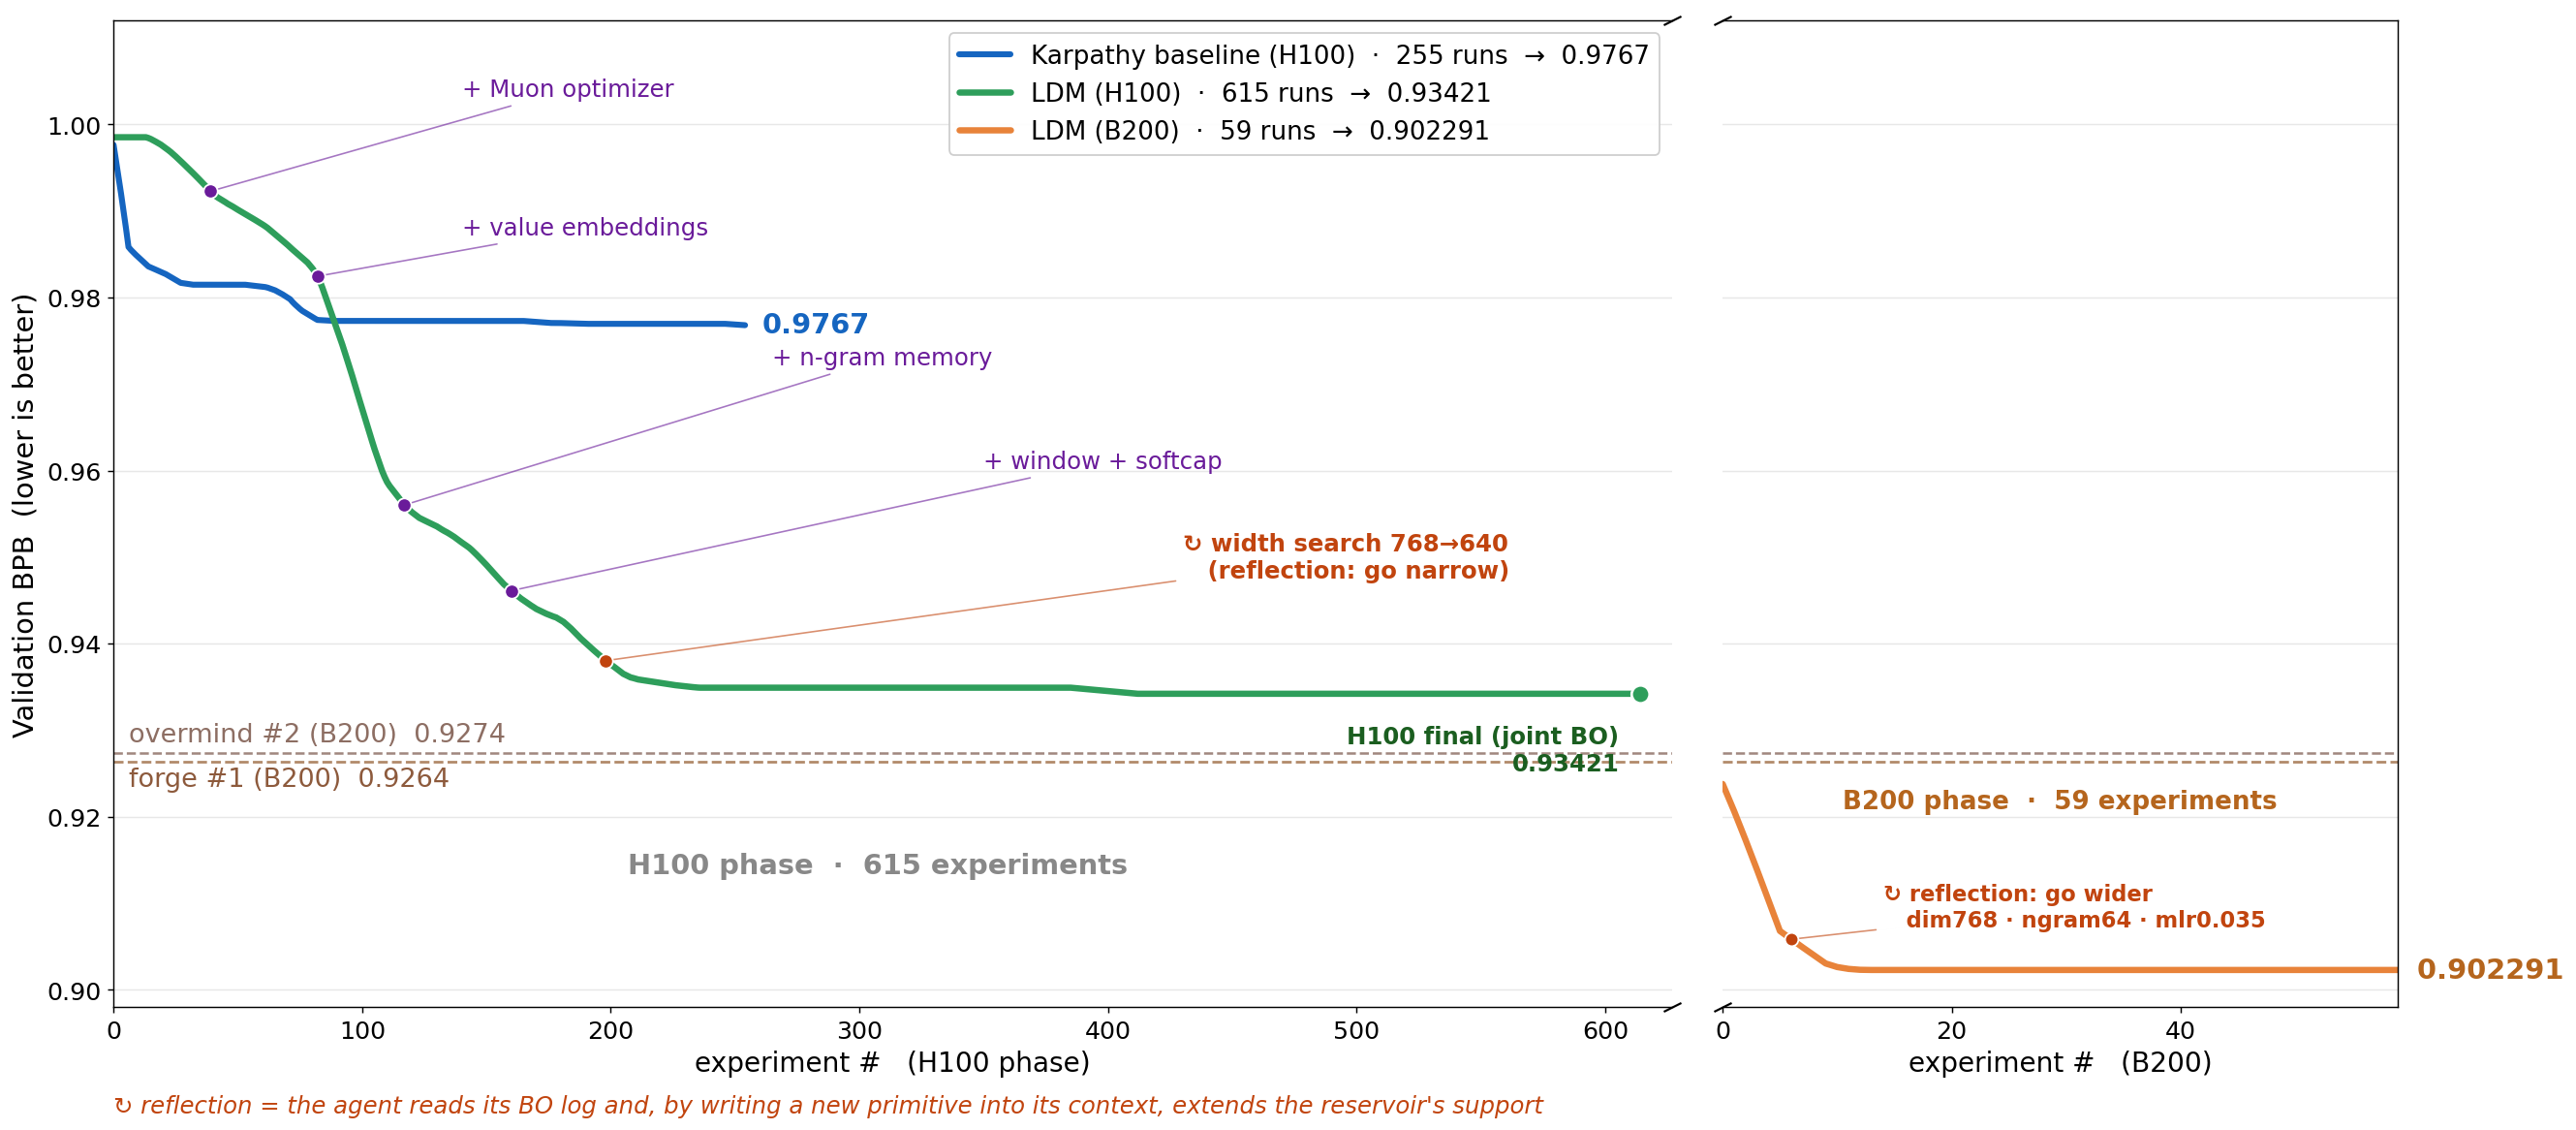
\includegraphics[width=0.95\linewidth]{figure/ldm_h100_b200.png}
    \caption{\textbf{The discover loop on \texttt{autoresearch}.} Validation \texttt{val\_bpb} (lower is better) versus search progress. The H100 panel compares the no-discover Karpathy baseline with the LDM; the B200 panel reports a matched-hardware leaderboard run of the LDM. B200 width scaled for legibility.}
    \label{fig:autoresearch}
\end{figure}

\begin{table}[ht]
\centering
\footnotesize
\begin{tabular}{@{}llr@{}}
\toprule
Change & Why it helps under a fixed time budget & $\Delta$\texttt{val\_bpb} \\
\midrule
$n$-gram hash memory             & memorises local $n$-gram patterns at zero FLOP     & $-0.0275$ \\
QK-norm                          & steadier steps, more learning per step             & $-0.0137$ \\
Narrower model (dim 768$\to$640) & cheaper steps $\Rightarrow$ more steps in 300\,s   & $-0.0109$ \\
Windowed attention + softcap     & cheaper attention $\Rightarrow$ more tokens/sec    & $-0.0108$ \\
Squared-ReLU                     & richer per-token MLP representation                & $-0.0087$ \\
Value embeddings                 & extra per-token signal at near-zero cost           & $-0.0079$ \\
Muon optimizer                   & orthogonalised gradients, more learning per token  & $-0.0048$ \\
\bottomrule
\end{tabular}
\caption{\textbf{The \texttt{autoresearch} run as physics-grounded discovery.} Each row lists a change the LDM retained under a fixed 300\,s budget, the physical mechanism by which it helps, and the resulting change in \texttt{val\_bpb}.}
    \label{tab:autoresearch-discovery}
\end{table}

We use Karpathy's public \texttt{autoresearch} project \citep{karpathy2026autoresearch} as a testbed for acquisition-guided LLM search. In \texttt{autoresearch}, a coding agent repeatedly modifies a single file, \texttt{train.py}; each candidate program is evaluated by training a small language model for a fixed five-minute budget and measuring validation bits per byte (\texttt{val\_bpb}, lower is better). The original system provides only the LLM proposal-and-evaluation loop, to which we add the surrogate and acquisition-guided search. Under the LDM notation, a program is a design $x$ with reward
\[
R(x)=-\texttt{val\_bpb}(x),
\]
where the agent conditioned on the current context defines the proposal distribution $p_\theta(\cdot\mid\mathcal C_t)$, and the accumulated program--performance pairs form the dataset $\mathcal D_t$ used to fit the surrogate. The benchmark is well suited to LDM: the search space is executable programs (a natural semantic proposal target), every proposal receives a quantitative but non-differentiable score from a real training run, the fixed schedule makes runs directly comparable under fixed hardware, and the full trace of edits, outcomes, and failures can be logged and ablated end to end.

\subsubsection{Experiment setting}

We instantiate LDM in the indirect-parameterisation mode: rather than generating raw program text, the LLM acts as a meta-planner that exposes the tunable degrees of freedom of \texttt{train.py} (learning rate, width, depth, and related hyperparameters) as a continuous search space, over which we establish a standard Gaussian process with an RBF kernel and fixed hyperparameters (kept fixed rather than fit, for stability in the small-data regime), giving a calibrated posterior mean and uncertainty $(\mu_t,\sigma_t)$; Expected Improvement (Eq.~\eqref{eq:ei}) serves as the acquisition function.

Each round the LLM proposes a pool of candidate configurations conditioned on $\mathcal C_t$, and the surrogate selects the next configuration to evaluate by maximising EI, with a diversity term for batched rounds. When the incumbent stalls, the reflection step lets the LLM re-parameterise the search space (i.e., adding or reshaping the tunable axes) before search resumes. The primary comparison holds the coding model, environment, and five-minute-per-run budget fixed, contrasting the original Karpathy LLM-only loop against the full LDM.

\subsubsection{Results}

Under a fixed context $\mathcal C_t$, acquisition-guided search exploits high-performing configurations and explores regions of high surrogate uncertainty. Figure~\ref{fig:autoresearch} shows the resulting \emph{descend--plateau--descend} pattern (i.e., improvement, plateau, then further improvement once reflection reshapes the search space) consistent with the intended search--stagnation--reflection cycle, though the learning curve alone does not establish causality. Under the same H100 five-minute-per-run schedule, the Karpathy LLM-only baseline plateaus at $\texttt{val\_bpb}\approx0.9767$ after about $255$ runs, whereas the full LDM continues improving to $0.93421$. This is a system-level comparison and is not intended to isolate any single component. The per-factor ablations appear in Section~\ref{sec:ablation-main} and Appendix~\ref{app:ablation}. Additionally, in Appendix~\ref{app:abl-pure-llm}, we also report the performance of the pure-LLM discovery loop, which identifies that quantification acquisition values are the central source of the LDM's advantage.

Separately, and independent of the mechanism above, Figure~\ref{fig:autoresearch} also reports a leaderboard result on B200 hardware for comparison with stronger public systems on the same accelerator. On B200 the LDM reaches $\texttt{val\_bpb}=0.902291$ in $59$ runs, surpassing the strongest public methods \textsc{forge} ($0.9264$) and \textsc{overmind} ($0.9274$) for top-1 on the \texttt{autoresearch@home} leaderboard.\footnote{\url{https://www.ensue-network.ai/lab/autoresearch}} Under the fixed training budget the model is token-bound, so \texttt{val\_bpb} falls only by training on more tokens or by learning more from each token; Table~\ref{tab:autoresearch-discovery} traces how each retained change does one or the other, taking \texttt{val\_bpb} from $0.9961$ to $0.902291$ ($-0.094$ overall), each attributable to a concrete physical mechanism rather than metric overfitting.


\subsection{Antibody CDRH3 design}
\label{sec:cs-antibody-results}

We select antibody CDRH3 loop design as our second case study because it represents a canonical high-dimensional combinatorial optimisation problem with a well-defined design space. The CDRH3 loop is the primary determinant of antibody binding specificity, with sequences of length \(L \approx 11\) drawn from 20 amino acids, yielding a discrete space of size \(20^{11}\). This setting falls into the \emph{known unknown} regime: the syntax and boundaries of the design space are fully specified, but the sequence-to-affinity mapping is unknown, highly rugged, and expensive to evaluate. Traditional combinatorial Bayesian optimisation methods struggle with the intractable size of this discrete space, while pure LLM generation lacks calibrated value guidance. The task therefore provides a clean testbed for evaluating how LDM combines structured proposal generation with calibrated acquisition guidance.

We use the \textsc{Absolut!} structure-based simulator as the black-box oracle, which returns a lattice binding energy \(E_{\mathrm{bind}}\) \citep{khan2022antbo}. We maximise \(R(x) = -E_{\mathrm{bind}}(x)\) since lower binding energy corresponds to stronger affinity, and each evaluation constitutes a single expensive oracle call.

\subsubsection{Experimental settings}

Experiments run sequentially, with one antibody candidate selected per iteration. We evaluate across five PDB targets, including 1ADQ\_A, 1FBI\_X, 1H0D\_C, 1NSN\_S, and 1OB1\_C, with a total budget of 200 evaluations per target, reporting mean performance and one standard deviation over multiple random seeds.

Baselines fall into four categories: \textbf{Pure LLM} (direct autoregressive sequence generation), combinatorial BO frameworks (\textbf{TURBO}, \textbf{COMBO}) adapted for discrete sequence spaces, the domain-specialised \textbf{AntBO} optimiser, and naive random search. We position LDM as a competitive general-purpose alternative rather than claiming to outperform the domain-specialised AntBO.

We implement four LDM variants formed by two orthogonal design choices: two LLM base generation strategies, paired with two acquisition weighting rules. Here \textbf{Policy} denotes the indirect parameterisation of \S\ref{sec:algo}: the LLM parameterises a sampling policy (with internal complexity), and the policy implicitly induces the base measure $p_{\theta,\alpha}(\cdot\mid\C_t)$. The \textbf{Direct} base measure generates sequences token-by-token with a small sample pool of \(m=5\). The \textbf{Policy} base measure lets the LLM output structured search parameters to spawn a much larger candidate pool. For weighting, \textbf{Max} picks the highest-acquisition candidate (mode approximation), while \textbf{Softmax} samples proportionally to exponentiated acquisition scores to approximate the full tilted distribution. Table~\ref{tab:ldm-variants-antibody} summarises all combinations.

\begin{table}[htbp]
    \centering
    \begin{tabular}{ccc}
        \hline
        LDM Variant & Base Measure \(p_\theta(x \mid \mathcal{C}_t)\) & Reduction Rule \\
        \hline
        Direct\_Max & Direct token-level sequence generation & Max \\
        Direct\_Softmax & Direct token-level sequence generation & Softmax \\
        Policy\_Max & Structured search policy from LLM output & Max \\
        Policy\_Softmax & Structured search policy from LLM output & Softmax \\
        \hline
    \end{tabular}
    \caption{Implemented LDM algorithm variants for computational antibody design.}
    \label{tab:ldm-variants-antibody}
\end{table}

\subsubsection{Results}

\begin{figure}[h!]
\centering
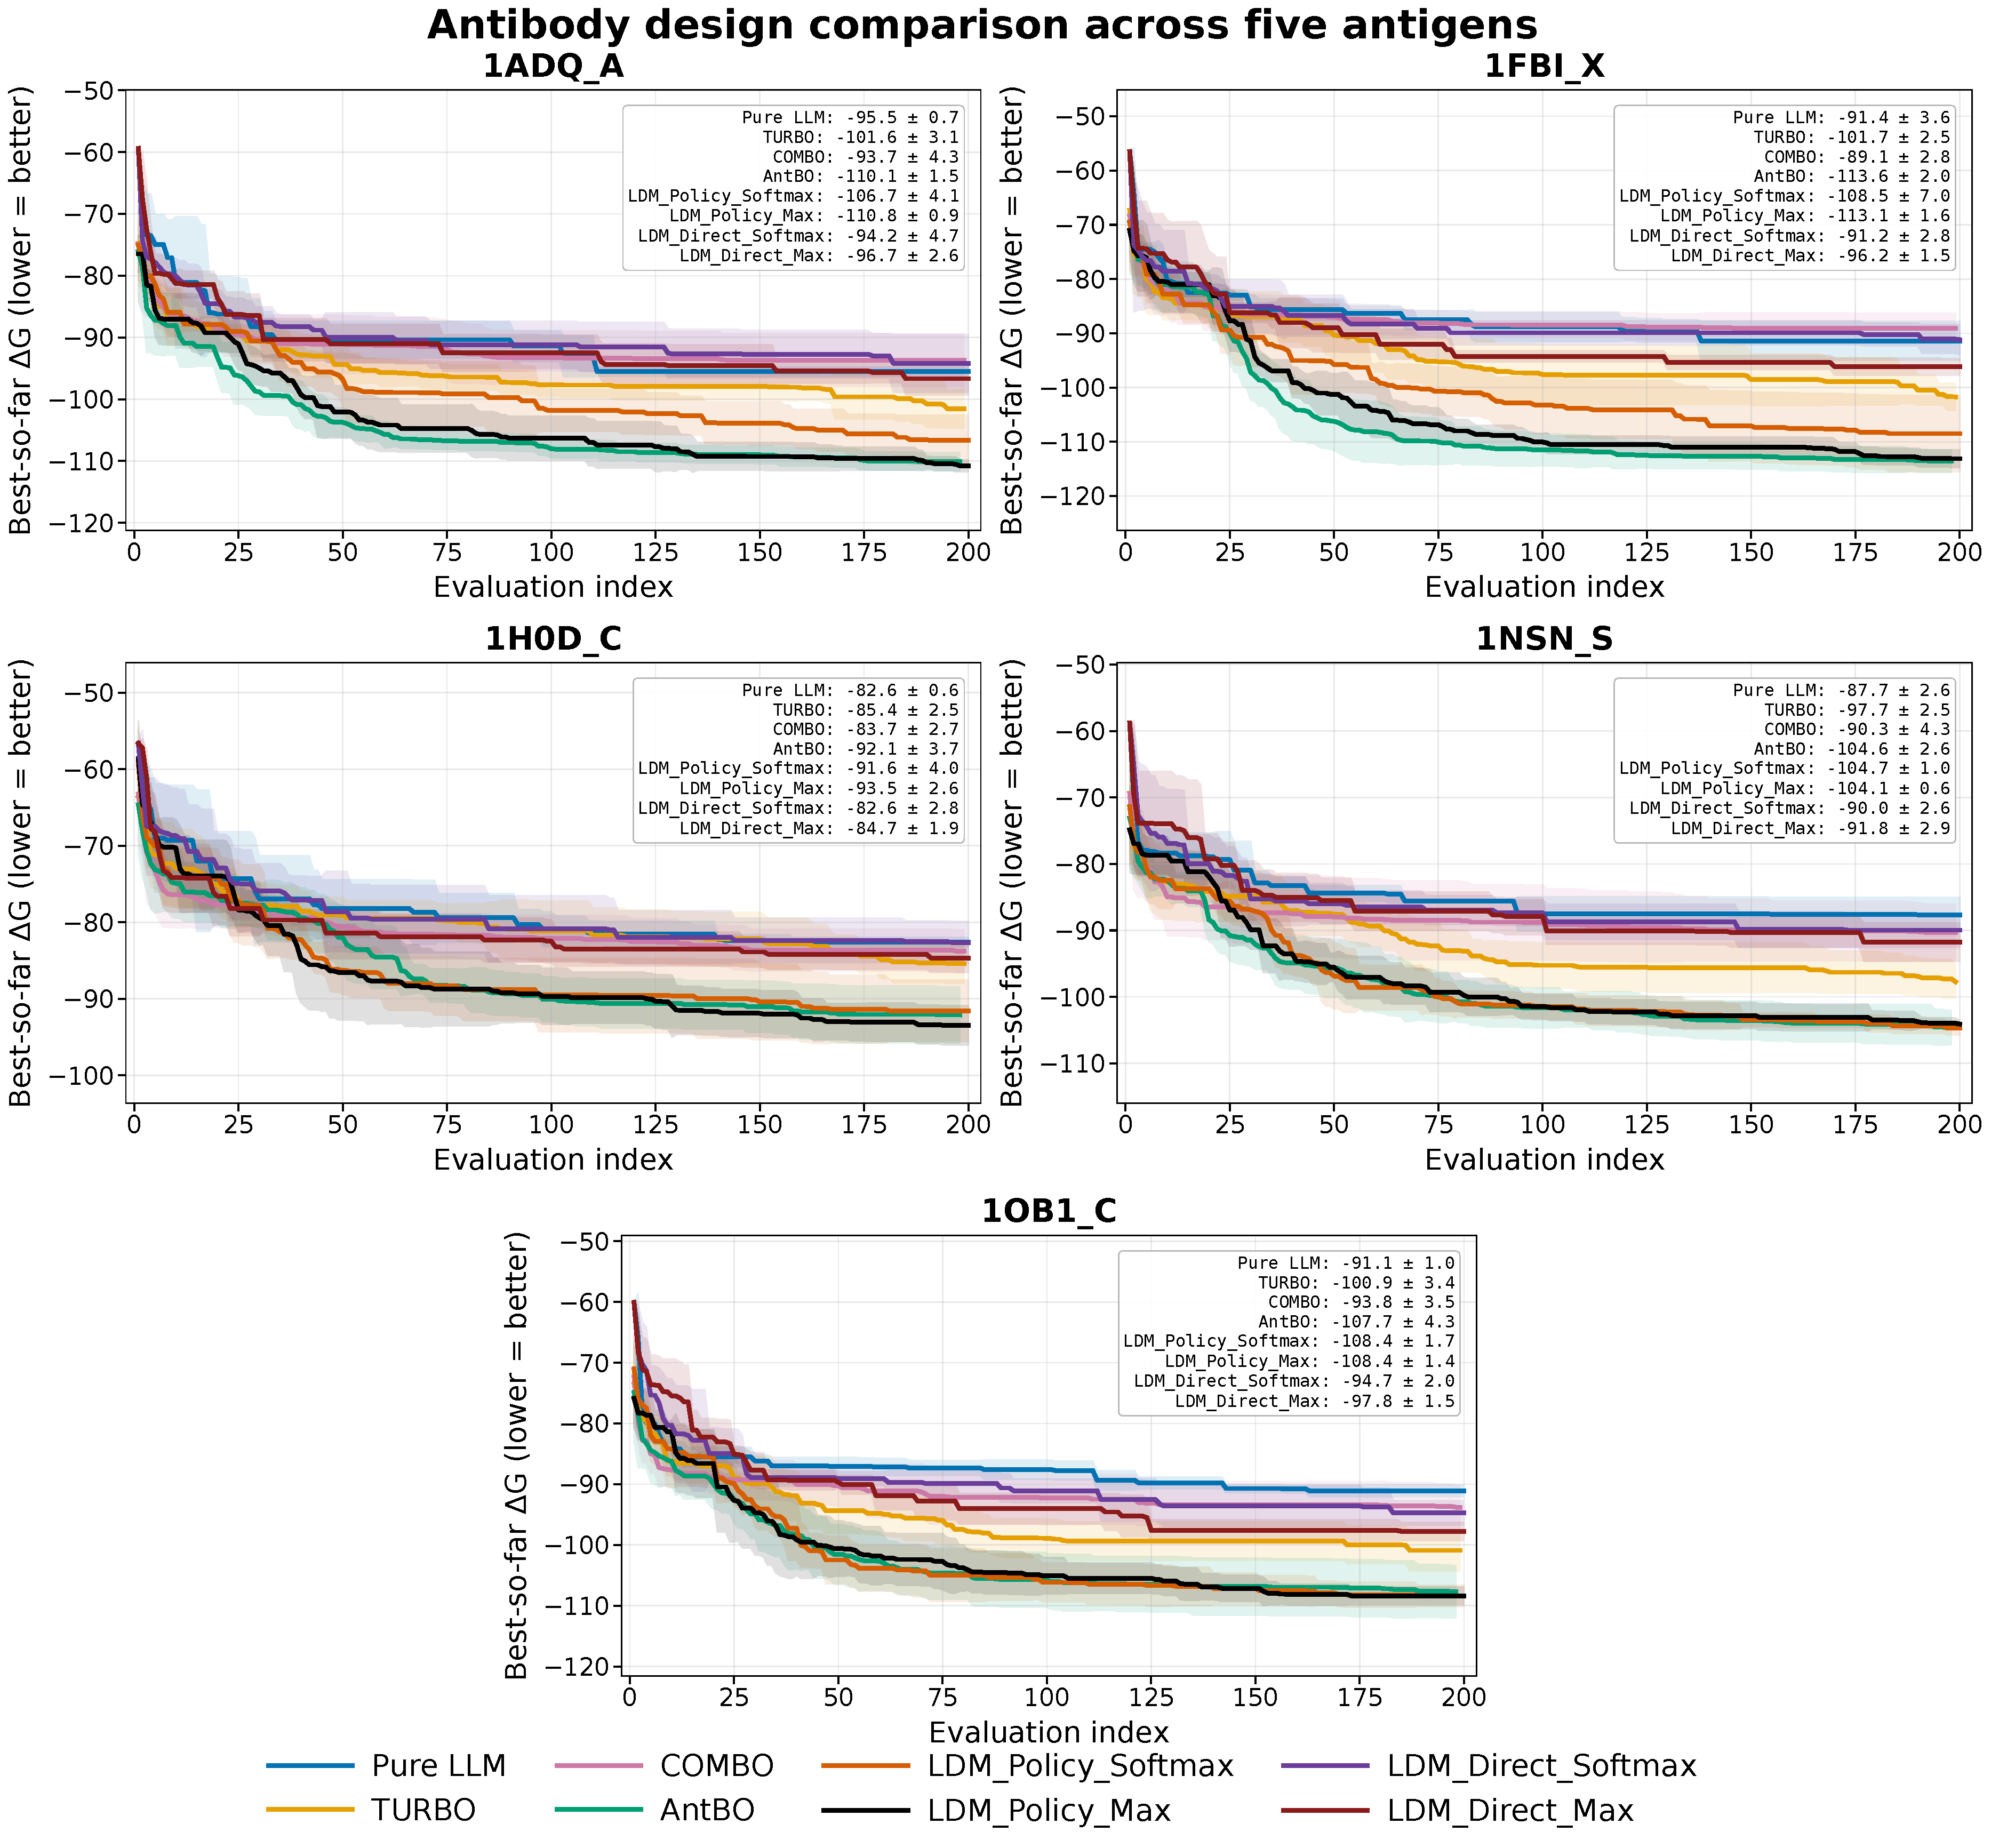
\includegraphics[width=1.0\linewidth]{figure/antibody_results.pdf}
\caption{Binding affinity performance across five antibody antigens. Axes: horizontal = number of sequence evaluations; vertical = best-so-far binding energy score (lower values indicate stronger binding). Curves correspond to all tested baselines and LDM variants.}
\label{fig:cs-antibody-results}
\end{figure}

Figure~\ref{fig:cs-antibody-results} compares all methods across the five protein targets. Policy-based LDM variants consistently outperform direct generation variants, achieving affinity levels comparable to AntBO, while Direct variants perform only marginally better than standalone LLMs.

Protein fitness landscapes are sparse and rugged, restricting the utility of small batches of directly generated sequences; even post-hoc acquisition reweighting cannot recover promising candidates the LLM fails to propose. In contrast, policy-mode LDM uses the LLM to define search regions rather than final sequences, expanding the candidate pool without extra oracle calls. This separation of semantic search scope planning (LLM) and calibrated value filtering (Bayesian surrogate) yields broader, more effective exploration of sequence neighbourhoods.

\begin{figure}[h!]
\centering
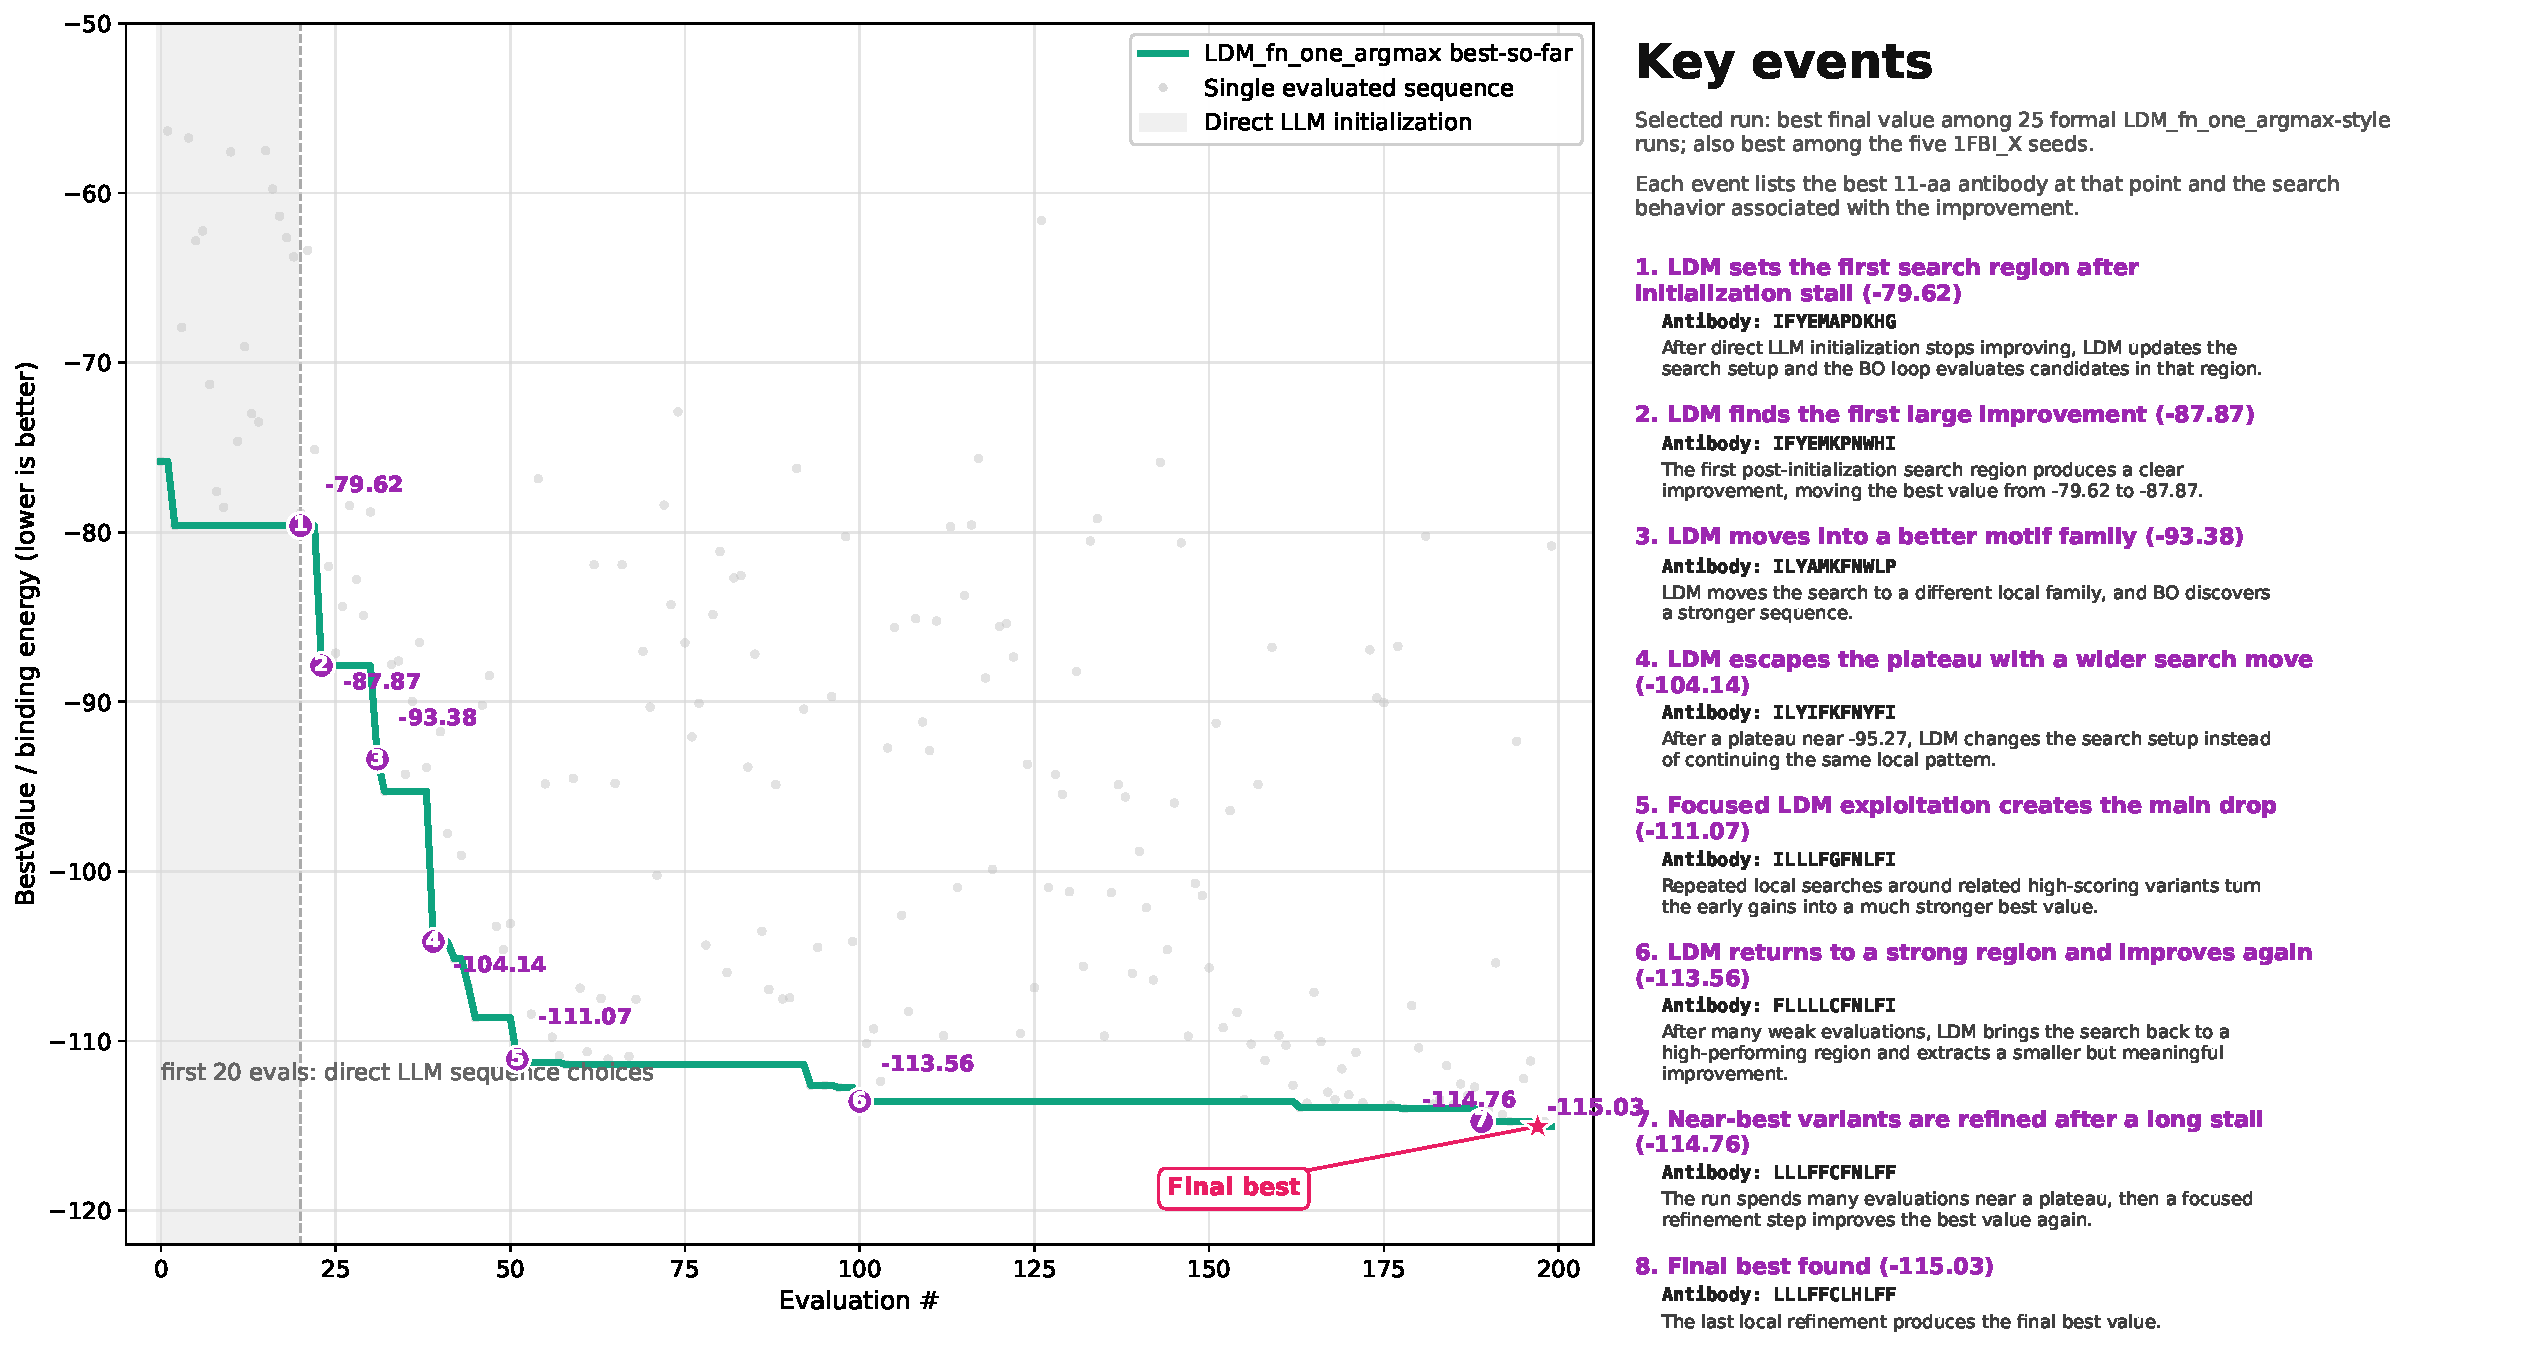
\includegraphics[width=0.95\linewidth]{figure/antibody_example_trajectory.pdf}
\caption{Optimisation trajectory of the top-performing LDM run on antigen 1FBI\_X. Horizontal axis counts evaluation rounds; vertical axis tracks the best binding energy found to date (lower = better). Step curve records global improvement milestones, with numbered markers highlighting major discovery events where the system introduces structurally novel sequence families after local plateaus.}
\label{fig:antibody_trajectory}
\end{figure}

Figure~\ref{fig:antibody_trajectory} visualises a representative LDM optimisation trajectory on the 1FBI\_X antigen, illustrating the core exploit–explore–discover cycle described in Section 2. Initial LLM sampling quickly hits a local performance ceiling; the LDM detects stagnation and triggers discovery steps to expand the sequence families under consideration. Each numbered marker denotes a discovery event that lifts the achievable performance ceiling, followed by phases of local refinement within the newly uncovered structural space.

% ============================================================
\subsection{Small-molecule drug discovery}
\label{sec:cs-molecule-results}

We select multi-objective small-molecule lead discovery as the third case study to test LDM’s handling of the \emph{unknown unknown} regime. Valid SMILES strings form an effectively unbounded chemical space with no clear global boundary, making full enumeration impossible. Standard multi-objective Bayesian optimisation (MOBO) with string kernels lacks strong structural priors and saturates rapidly. Auxiliary expansion tools such as ReaSyn only generate analogues around fixed seed molecules, limiting exploration to narrow local chemical neighbourhoods. This domain therefore benchmarks LDM’s unique capability to autonomously uncover entirely novel molecular scaffolds outside initial seed support.

Our multi-objective task optimises two conflicting rewards for the KRAS G12D target \citep{kumarOverviewKRASG12D2026}: AutoDock Vina \citep{trott2010AutoDockVina} docking score (\(R_{\mathrm{Vina}}\), minimise) and neural-network binding activity (\(R_{\mathrm{act}}\), maximise). We quantify performance via the hypervolume of the Pareto front, with a fixed reference point across all experiments and a total evaluation budget of 80 iterations.

\subsubsection{Experimental settings}

Independent Gaussian Process surrogates are fitted for each reward dimension, with the subsequence string kernel measuring SMILES structural similarity. Expected Hypervolume Improvement (EHVI) serves as the multi-objective acquisition function. Baselines include vanilla MOBO and random search. We evaluate two LDM instantiations sharing the same tilted sampling pipeline but differing in candidate pool construction:
\begin{enumerate}
    \item \textbf{Direct-Softmax}: The LLM generates large parallel batches of 128 raw SMILES candidates for acquisition-weighted resampling.
    \item \textbf{ReaSyn-Softmax}: The LLM outputs a small set of seed SMILES, with ReaSyn generating local analogues to build the candidate pool before softmax selection.
\end{enumerate}

\subsubsection{Results}

\begin{figure}[h!]
\centering
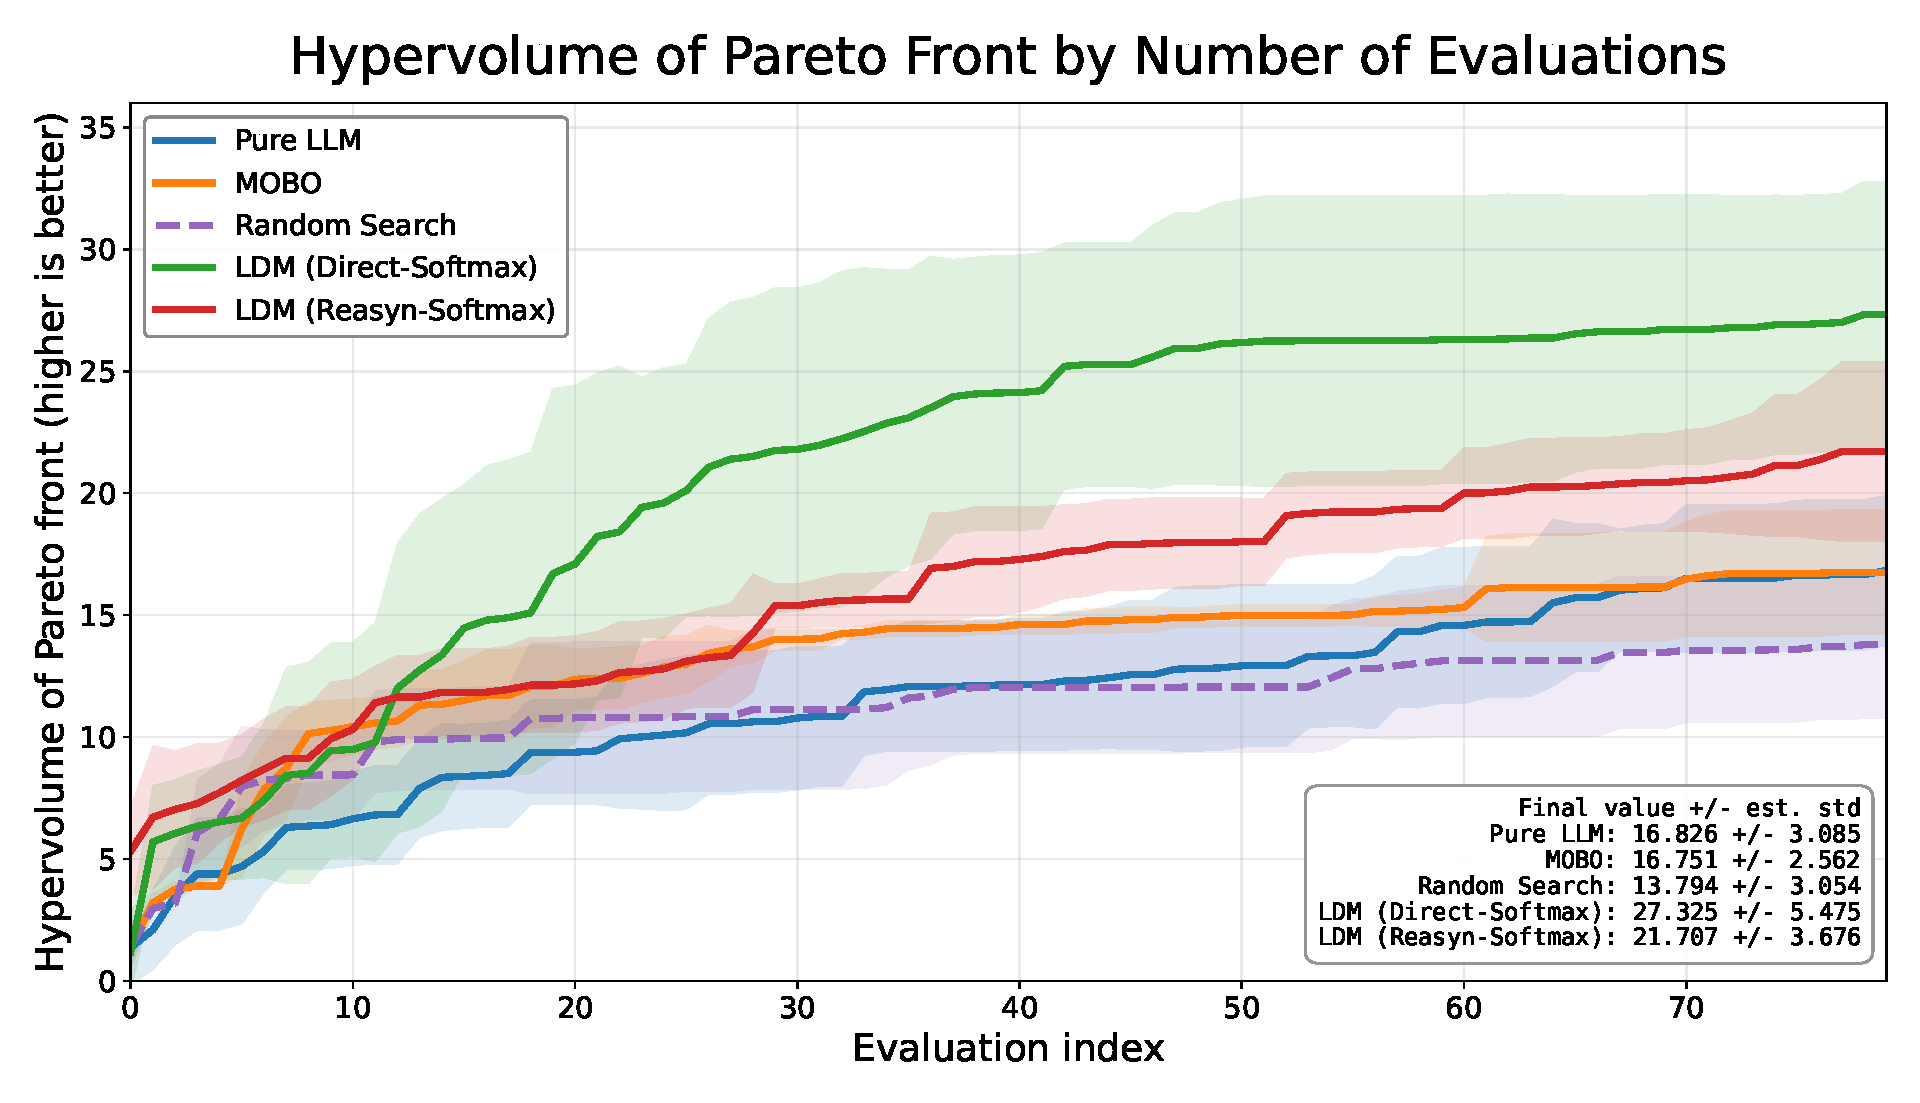
\includegraphics[width=0.6\linewidth]{figure/molecule_results.pdf}
\caption{Pareto hypervolume growth for molecular design. Horizontal axis = evaluation count; vertical axis = dominated hypervolume of the Pareto front (higher values denote better multi-objective trade-offs). Separate curves track performance of random search, standard MOBO, and the two LDM variants.}
\label{fig:cs-molecule-results}
\end{figure}

Figure~\ref{fig:cs-molecule-results} shows that both LDM variants outperform all baselines by a substantial margin, with Direct-Softmax delivering the strongest hypervolume gains. Conventional MOBO plateaus after roughly 40 evaluations, trapped within limited chemical regions, while direct LLM generation sustains steady front expansion across the full budget.

The performance gap between the two LDM variants arises from a breadth–synthesizability trade-off. General-purpose LLMs carry broad pre-training knowledge of diverse SMILES structures; large-batch direct generation unlocks wider scaffold exploration. ReaSyn’s local analogue generation improves synthetic tractability but restricts structural diversity, slowing Pareto expansion for early-stage lead discovery where novel scaffolds are prioritised.

\begin{figure}[h!]
\centering
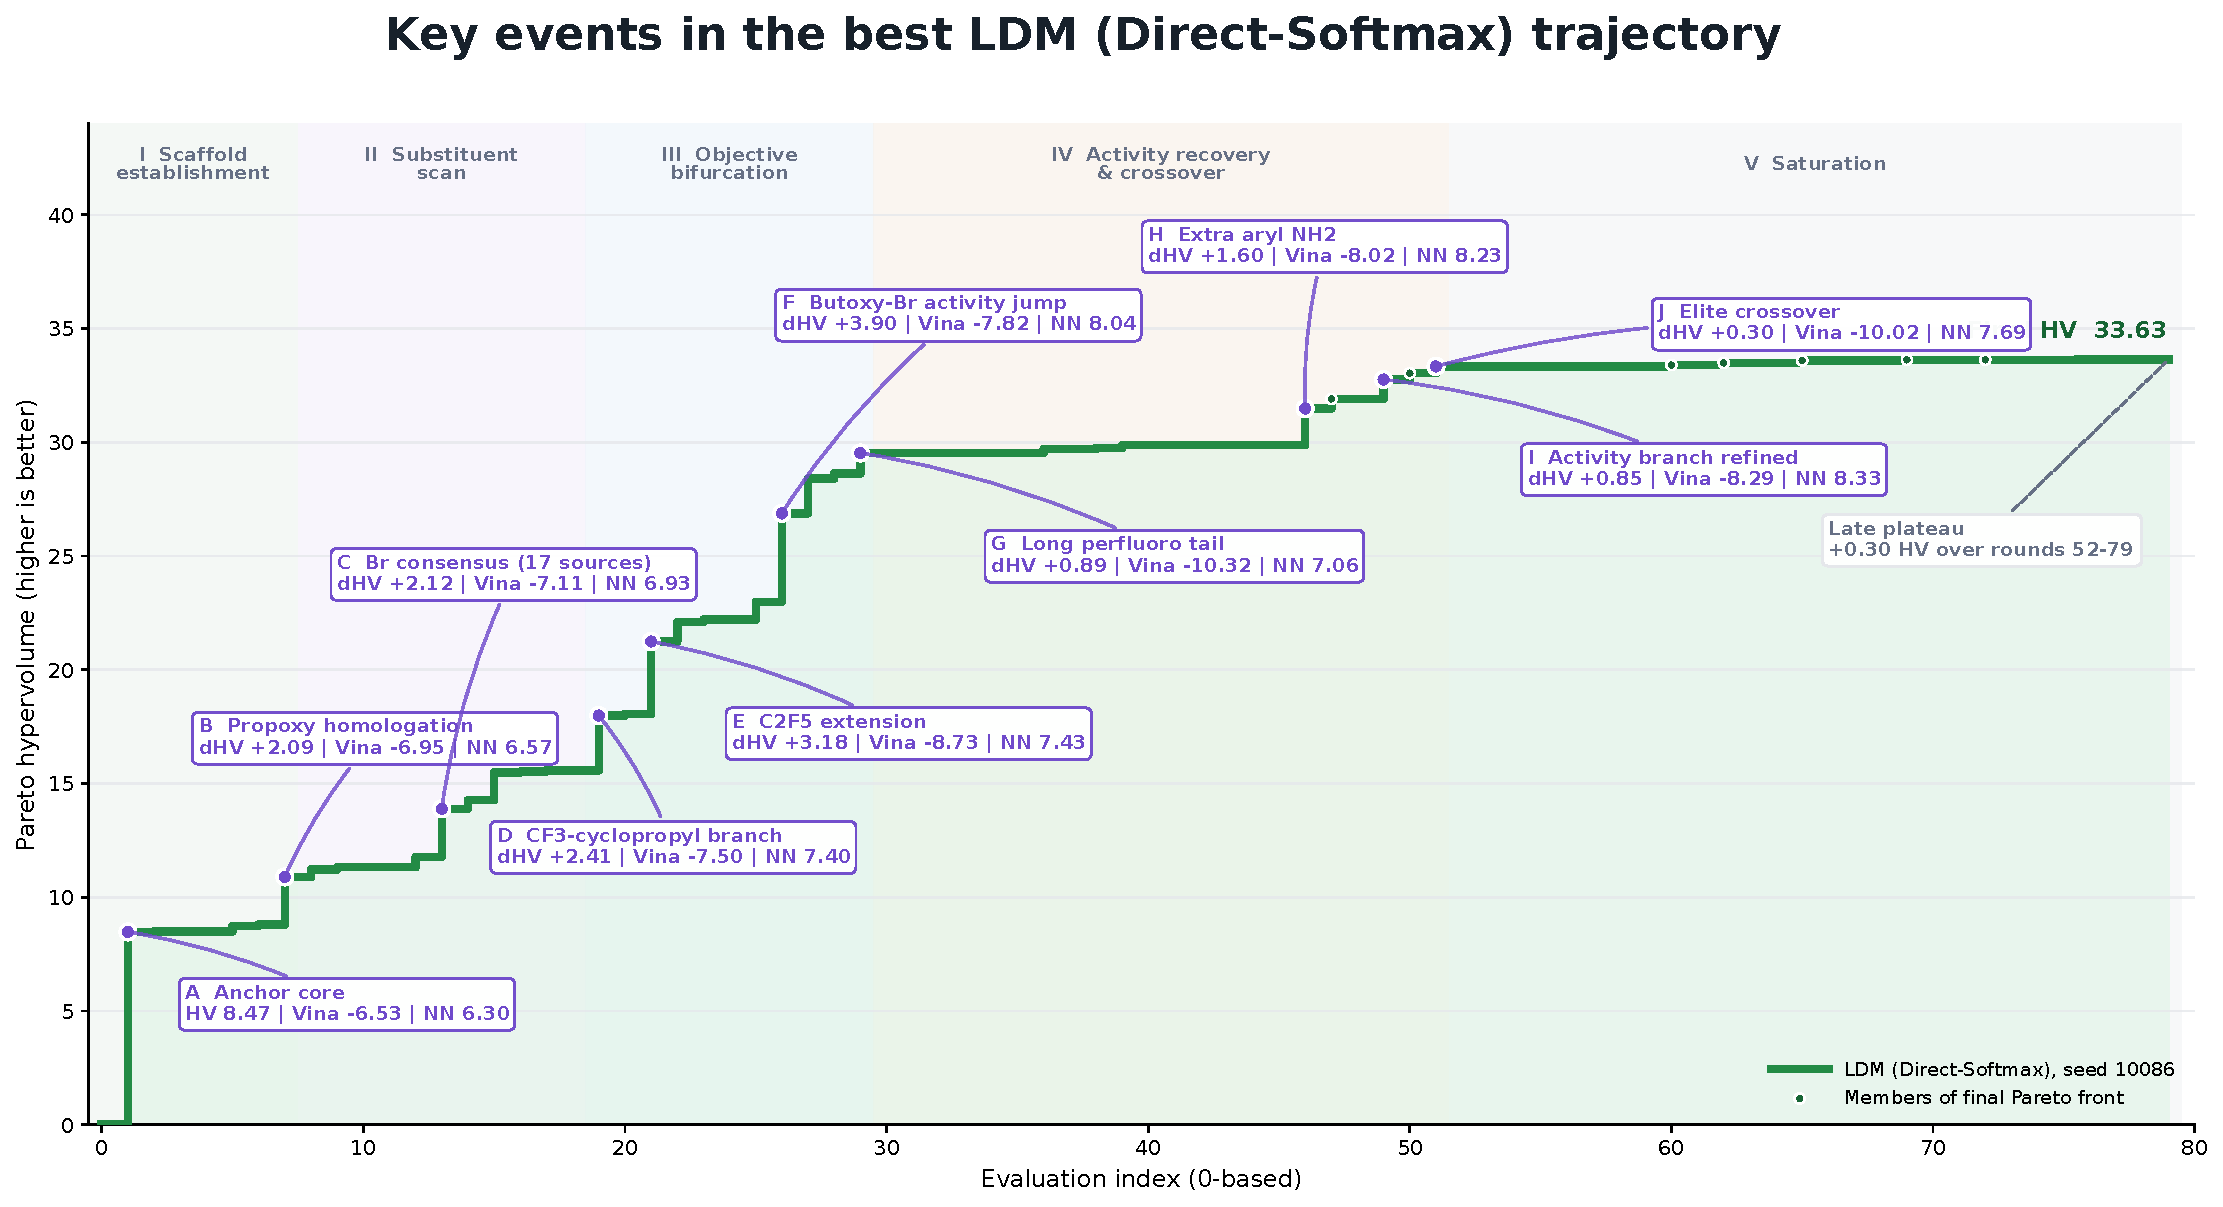
\includegraphics[width=1.0\linewidth]{figure/molecule_example_trajectory.pdf}
\caption{Key milestone events along a Direct-Softmax molecular optimisation trajectory. X-axis counts evaluation steps; Y-axis plots cumulative Pareto hypervolume (higher = better). Step curve tracks global front improvements, with labelled markers denoting structural discovery events that open new families of active molecules. Shaded bands partition the optimisation into five sequential search phases. In each text box, \texttt{HV} represents Hyper-Volumn, \texttt{Vina} represents the score of Autodock Vina, and \texttt{NN} represents the neural network as the oracle activity prediction.}
\label{fig:direct_softmax_key_events}
\end{figure}

\begin{figure}[h!]
\centering
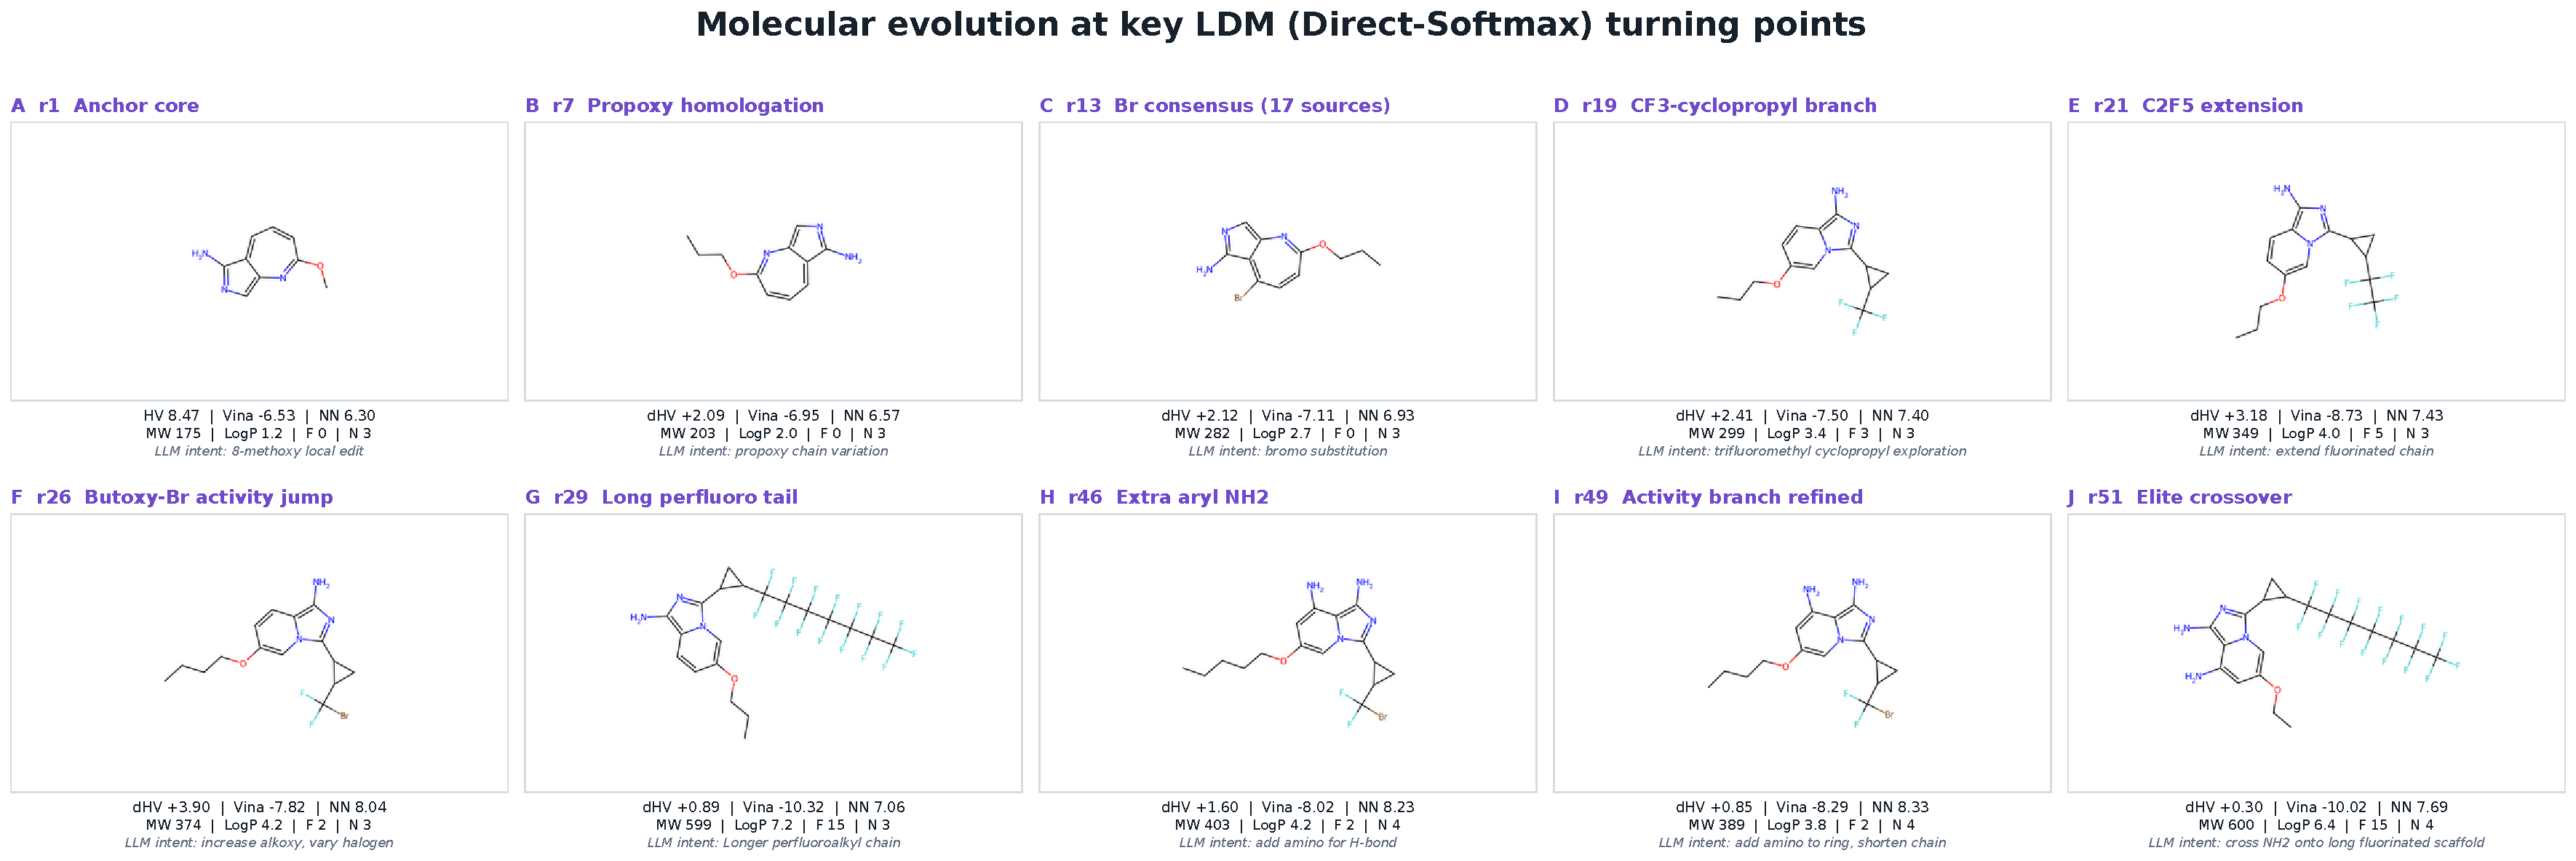
\includegraphics[width=1.0\linewidth]{figure/molecule_example_key_smiles.pdf}
\caption{Two-dimensional molecular structures corresponding to the ten core discovery milestones labelled in Figure~\ref{fig:direct_softmax_key_events}. Each structure is generated from canonical trajectory SMILES strings, arranged in chronological order of discovery to visualise the evolution of core chemical scaffolds and functional group substitutions.}
\label{fig:direct_softmax_molecular_evolution}
\end{figure}

Figures~\ref{fig:direct_softmax_key_events} and~\ref{fig:direct_softmax_molecular_evolution} together illustrate a complete LDM discovery workflow for small molecules. The hypervolume curve partitions optimisation into distinct stages: initial scaffold identification, substituent screening, objective bifurcation into docking- and activity-focused chemotypes, cross-family feature recombination, and final fine-tuning. The structural plot tracks how the model iteratively uncovers unrelated molecular backbones, a capability absent from standard BO or seed-local expansion tools.

%==============================finetune exp

\subsection{Fine-Tuning Experiments}
\label{sec:finetune-experiments}

We evaluate discovery fine-tuning across three structured design domains: multi-turn program search in AutoResearch, combinatorial antibody CDRH3 design, and multi-objective molecular discovery. In every experiment, the fine-tuned proposer is placed inside the same acquisition-guided LDM loop as the base proposer. Fine-tuning therefore changes the proposal reservoir, whereas the online surrogate continues to provide value and uncertainty estimates from the current experimental history.

We compare action-only discovery fine-tuning with reasoning-augmented fine-tuning. The latter trains the proposer to generate a surrogate-grounded research-progress rationale before emitting the candidate action.
\begin{figure*}[h!]
    \centering
    % Replace this path with the existing appendix path once located.
    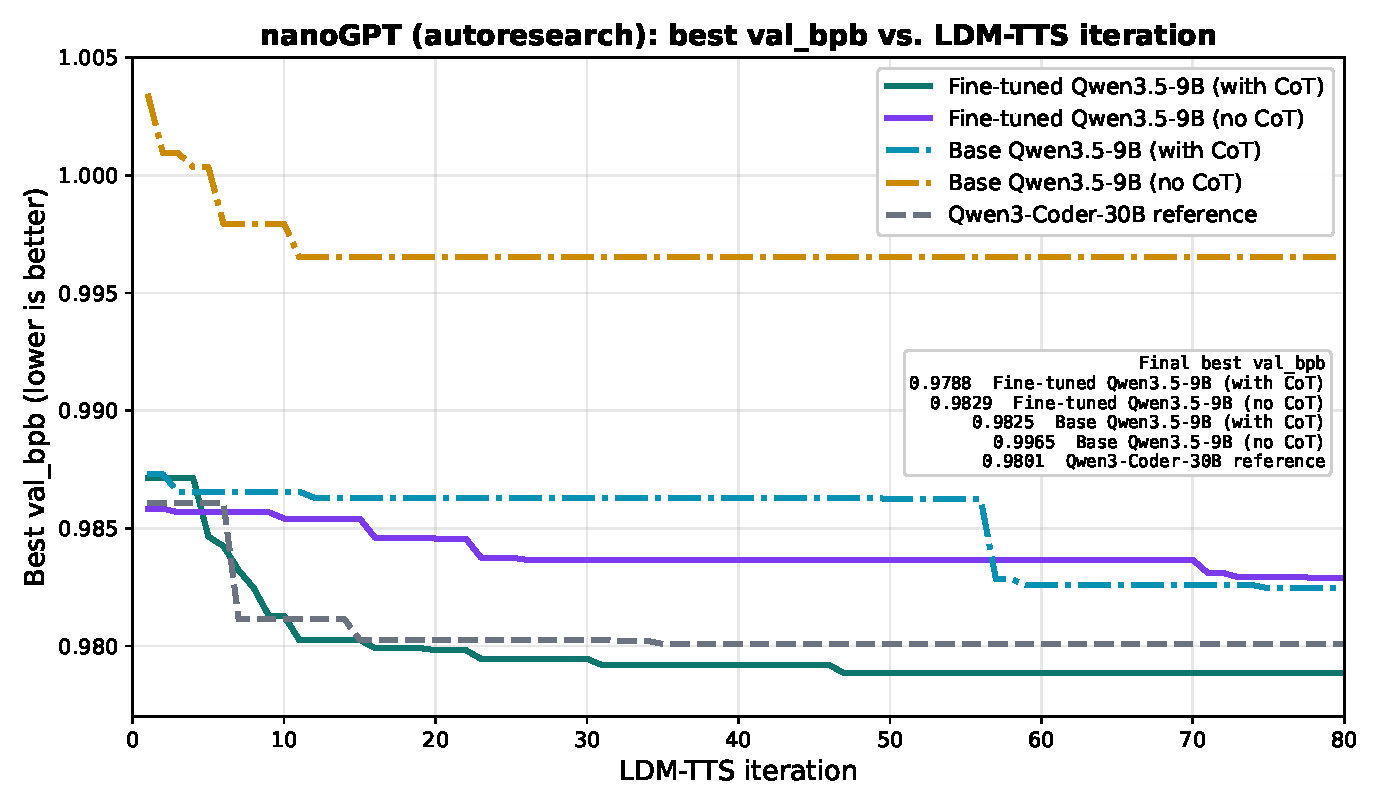
\includegraphics[width=0.82\textwidth]{figure/nanogpt_finetune_cot.pdf}
    \caption{\textbf{Reasoning-augmentation ablation on AutoResearch.} Best validation bits-per-byte (lower is better) versus LDM-TTS iteration inside an identical acquisition-guided loop, comparing fine-tuned and base proposers with and without reasoning augmentation and the Qwen3-Coder-30B reference.}
    \label{fig:finetune-autoresearch}
\end{figure*}

\subsubsection{AutoResearch}

We first study fine-tuning in AutoResearch, where an agent repeatedly edits a persistent training program and evaluates each proposal through a fixed-budget nanoGPT training run. This setting requires the model to interpret an evolving experiment ledger, recognize performance plateaus, and propose changes that test new program mechanisms.

Figure~\ref{fig:finetune-autoresearch} compares fine-tuned and base Qwen3.5-9B proposers over 80 LDM-TTS iterations. The reasoning-augmented fine-tuned model achieves the best validation performance, reaching $\mathrm{val\_bpb}=0.9788$, lower than the Qwen3-Coder-30B reference at $0.9801$. Fine-tuning without reasoning reaches $0.9829$, the base model with reasoning reaches $0.9825$, and the base model without reasoning stalls at $0.9965$. These results show that fine-tuning improves the program-search reservoir and that the explicit research-progress trace further helps the model escape local program families.

\subsubsection{Antibody CDRH3 Design}

We next evaluate antibody CDRH3 design, where the proposer searches a sparse and rugged sequence space under a limited binding-energy evaluation budget. We compare fine-tuned and base Qwen3.5-9B models with and without reasoning augmentation across five antigens. All variants use the same acquisition-guided LDM loop with expected-improvement acquisition and the same parallel evaluation budget.

Figure~\ref{fig:finetune-antibody} shows that fine-tuning improves over the corresponding base proposer across the five antigens. Both fine-tuned variants achieve lower binding energies than the base models, while the reasoning-augmented fine-tuned model obtains the lowest average binding energy among the four configurations. This result indicates that the distilled policy improves sequence-family proposals even in a large discrete design space.

\begin{figure*}[h!]
    \centering
    % Replace this path with the existing appendix path once located.
    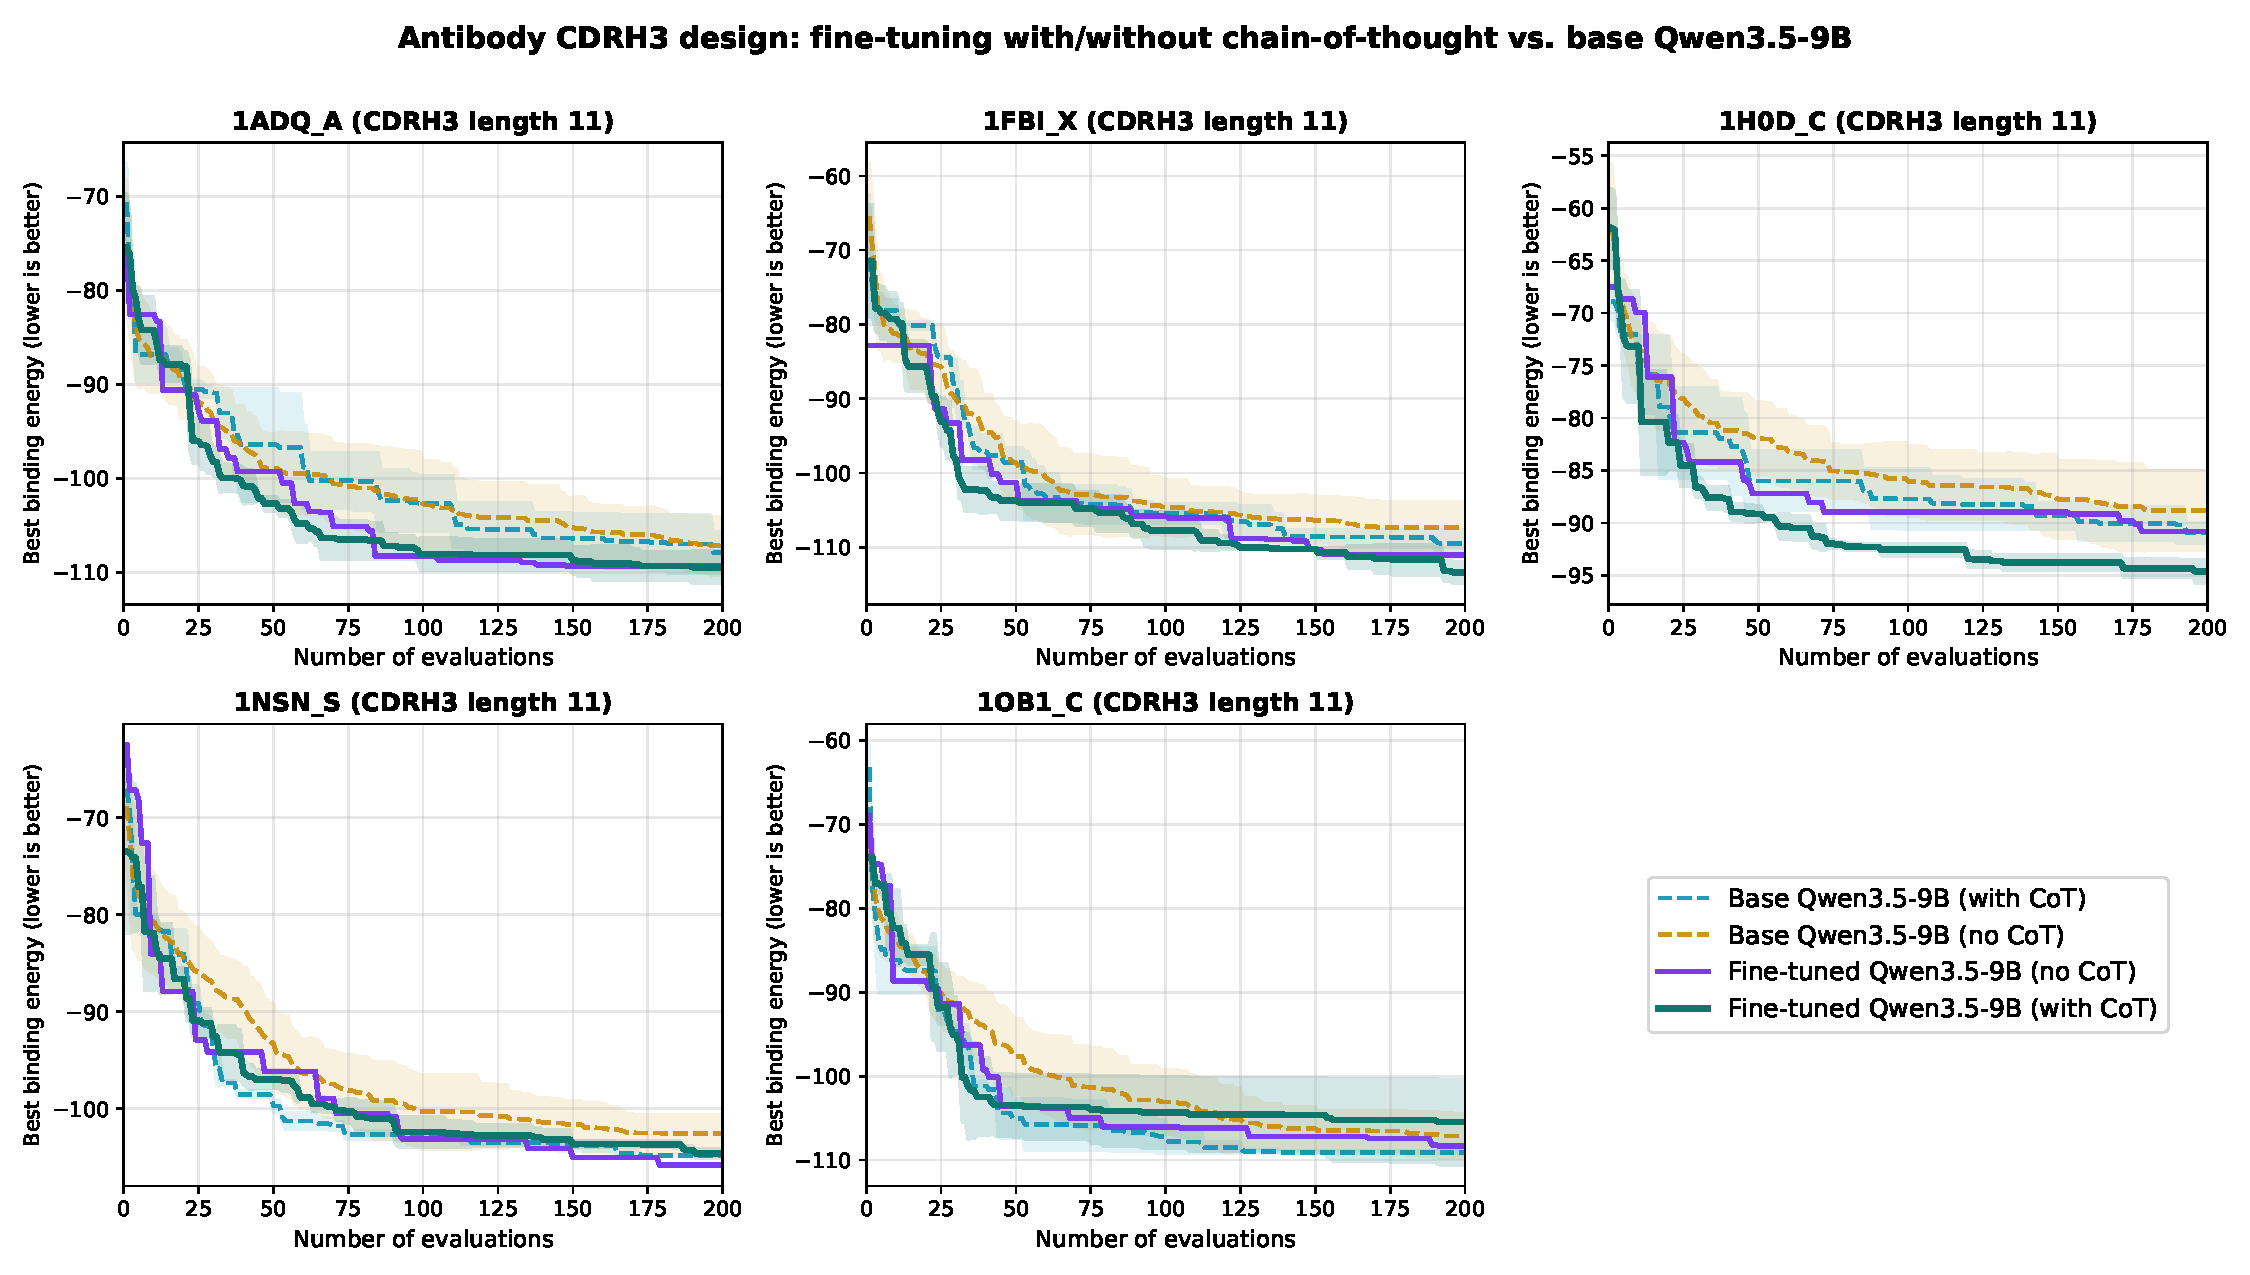
\includegraphics[width=0.94\textwidth]{figure/protein_finetune_cot.pdf}
    \caption{\textbf{Discovery fine-tuning for antibody CDRH3 design.} Best Absolut! binding energy, lower is better, versus the number of evaluations across five antigens. Fine-tuned Qwen3.5-9B variants with and without reasoning augmentation are compared with their corresponding base proposers in the same acquisition-guided LDM loop. Shaded bands denote mean $\pm$ standard deviation across available seeds.}
    \label{fig:finetune-antibody}
\end{figure*}

\subsubsection{Multi-objective Small-Molecule Discovery}

Finally, we evaluate cross-task transfer on the KRAS G12D molecular-design task. The task jointly optimizes docking and neural activity, and performance is measured by best-so-far Pareto-front hypervolume over 80 expensive evaluations.

Figure~\ref{fig:finetune-molecule} compares five inference-time policies inside the same LDM loop. The reasoning-augmented fine-tuned Qwen3.5-9B model achieves the highest final hypervolume, $26.660 \pm 2.608$. It exceeds the same fine-tuned student without reasoning, $22.279 \pm 3.828$, and both DeepSeek V4 Flash teacher variants, which reach $24.548 \pm 3.589$ with reasoning and $23.582 \pm 2.832$ without reasoning. The untuned Qwen3.5-9B base proposer reaches $16.489 \pm 5.867$. The result shows that the distilled policy transfers beyond the source task and that reasoning augmentation substantially improves this transfer.

\begin{figure*}[h!]
    \centering
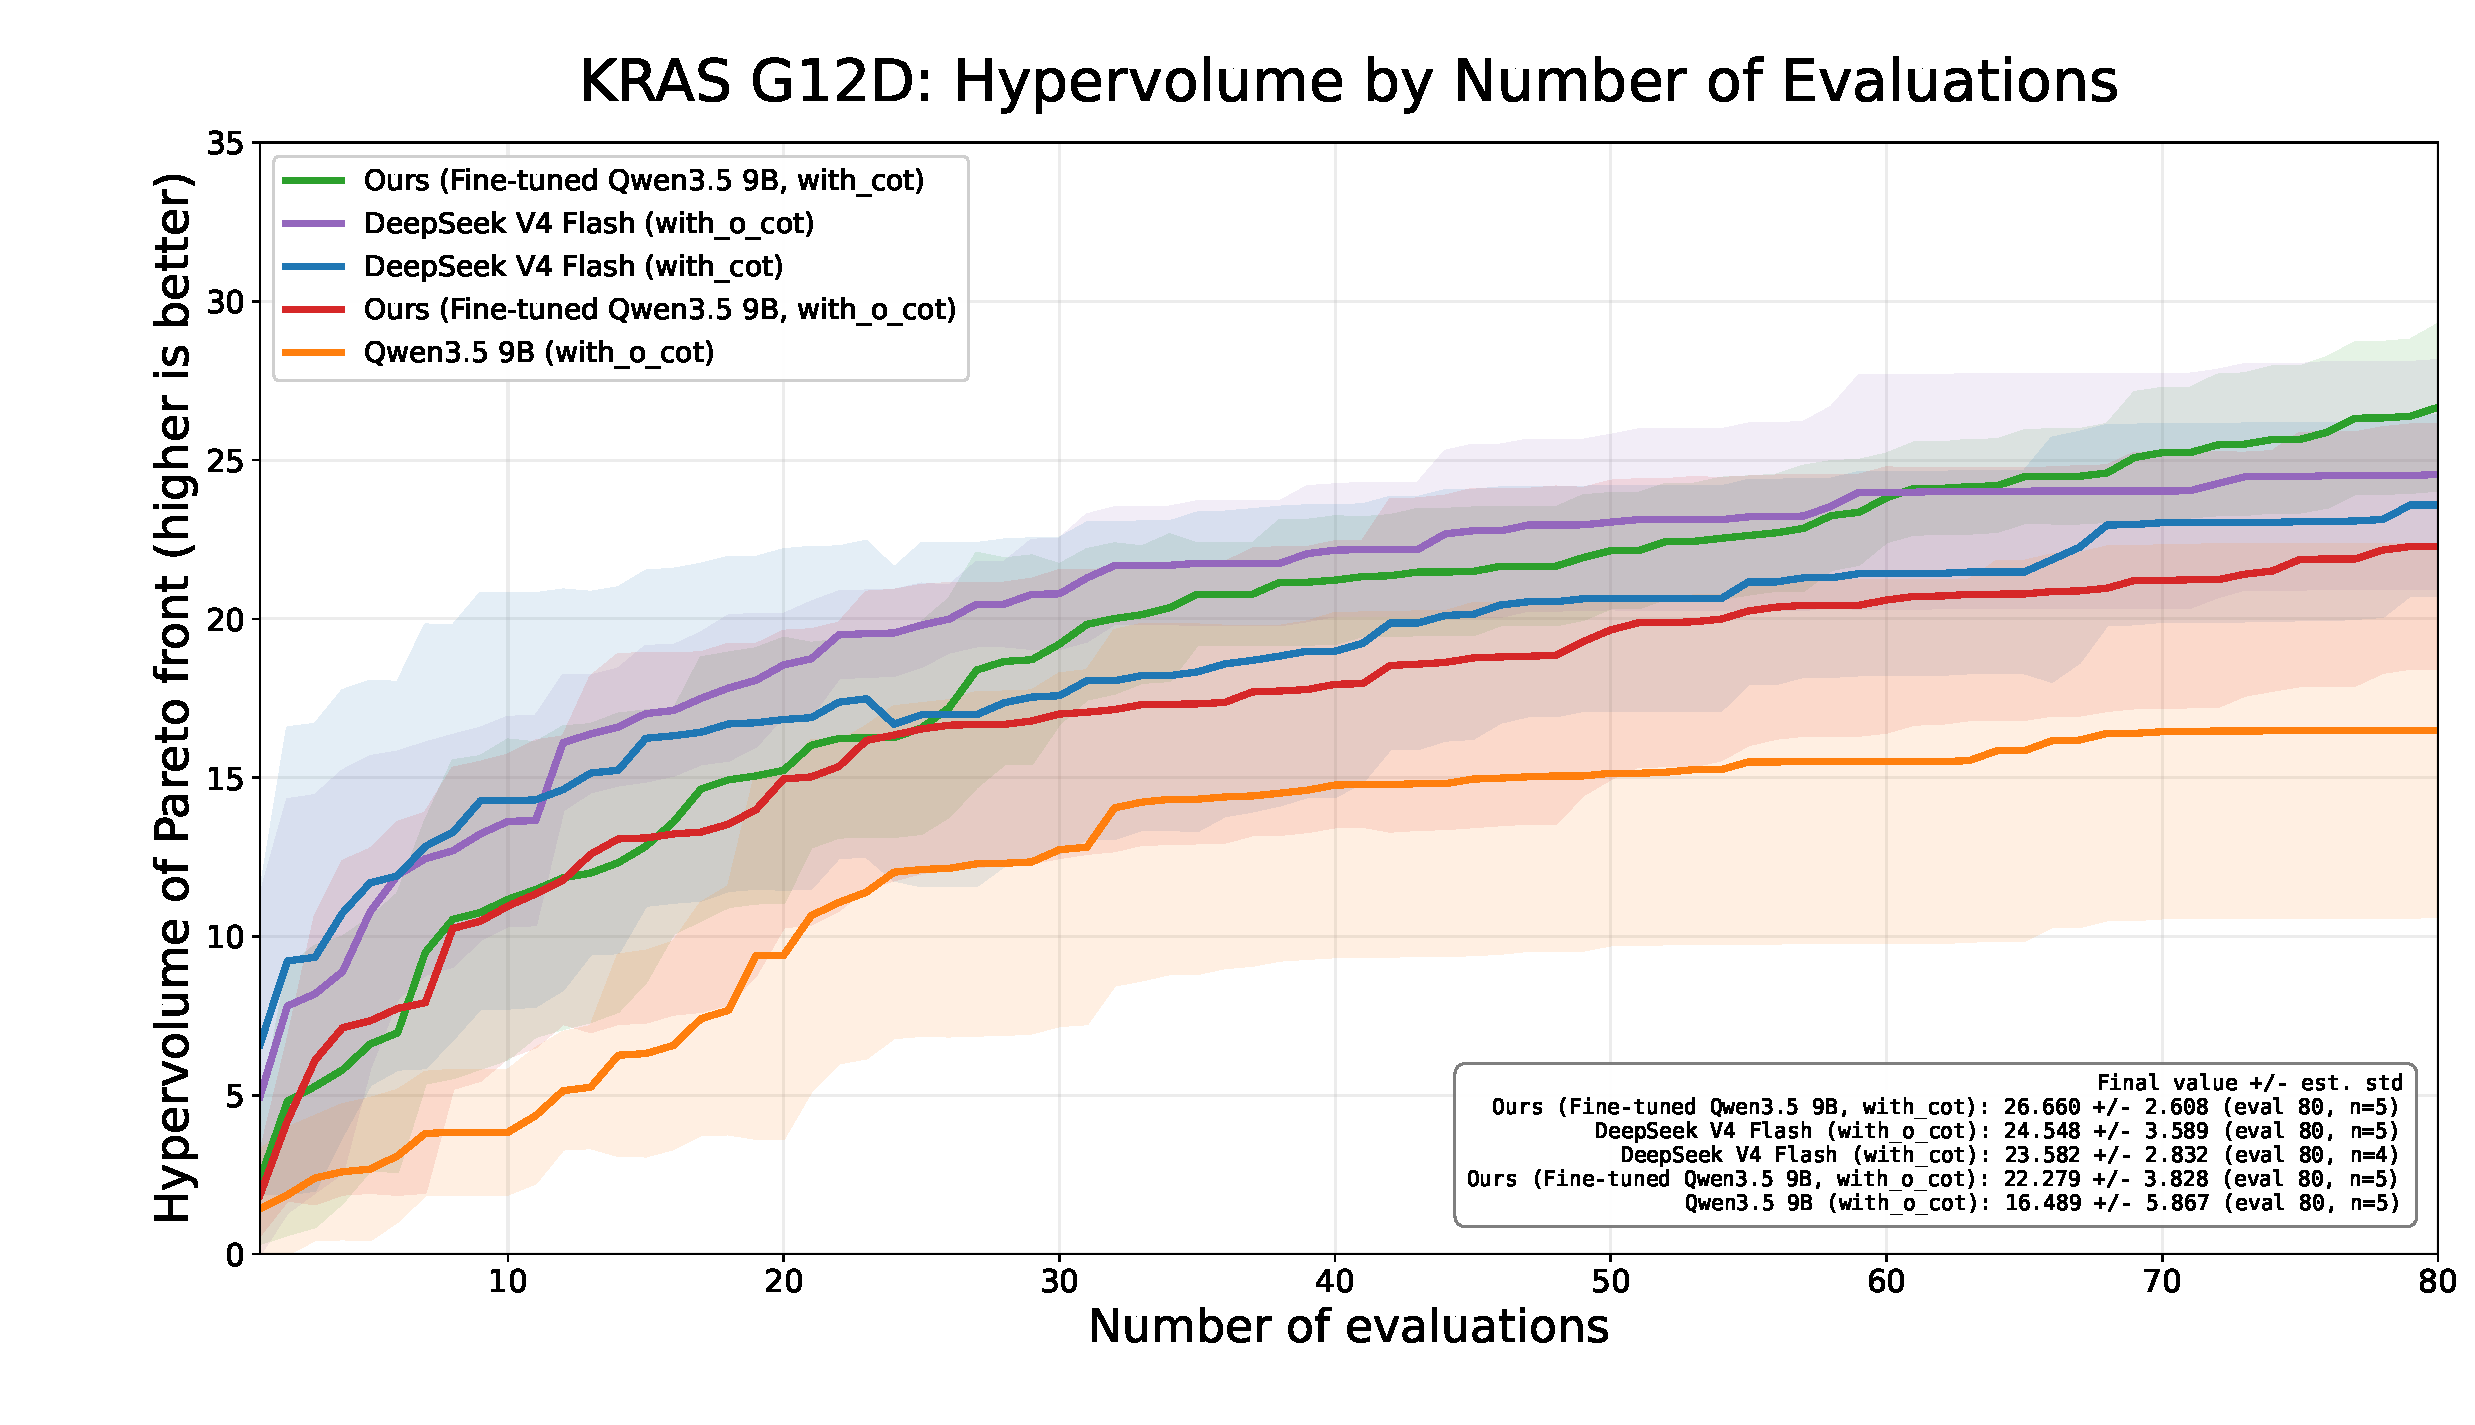
\includegraphics[width=0.82\textwidth]{figure/ldm_sft_small.pdf}
    \caption{\textbf{Fine-tuning with reasoning-augmented discovery data on KRAS G12D.} Best-so-far Pareto-front hypervolume (higher is better) versus the number of expensive evaluations, comparing fine-tuned and base proposers inside the same LDM loop. Shaded bands denote one standard deviation.}
    \label{fig:finetune-molecule}
\end{figure*}

Across programs, biological sequences, and molecules, fine-tuning improves the proposal reservoir within the online LDM loop. The gains are strongest when the model is trained to represent not only the next action but also the surrogate-grounded rationale for why that action advances scientific search.
% ============================================================
\subsection{Ablation Studies}
\label{sec:ablation-main}

The three case studies above have demonstrated the effectiveness of LDM in the spaces of programmes, biological sequences, and small molecules. In this section, we further conduct ablation experiments to investigate how LDM's gains depend on the test-time compute spent before each expensive evaluation, and how sensitive the policy is to its two temperature knobs $\alpha$ (LLM sampling temperature) and $\eta$ (acquisition tilt). Note that only partial ablation results are reported here; the remaining ablations results, including the pure LLM research loop on \texttt{autoresearch} with no BO value at all (\S\ref{app:abl-pure-llm}), the antibody CDRH3 hyperparameter sweep on $1\mathrm{NSN\_S}$, and the molecule and CDRH3 single-step budget sweeps (\S\ref{app:abl-ldm}), are reported in Appendix~\ref{app:ablation}.

\subsubsection{Test-time search scaling and acquisition functions}

We first ask whether LDM exhibits the same test-time scaling behaviour that motivates inference-time search in language-model reasoning \citep{snell2025scaling}, but in the harder setting where the value is an expensive scientific objective approximated by a surrogate. We keep the outer five-minute training budget fixed and vary only the cheap inner-loop budget of test-time search. The inner budget has two knobs: $N$ is the number of candidate \texttt{train.py} programs the LLM proposes at each outer iteration, and $H$ is the number of hypothesis/refinement branches each candidate is expanded into before the surrogate scores it; together they control the total acquisition-scored nodes per outer round, which we label \textsc{N$m$H$n$} so that \textsc{N4H4} scores $4 \times 4 = 16$ nodes per round and \textsc{N8H8} scores $8 \times 8 = 64$. We additionally vary whether the surrogate uses a fixed or dynamically expanded program-feature representation and which acquisition is used as the value (posterior mean only, EI, or an uncertainty-aware value).

\begin{figure}[htbp]
    \centering
    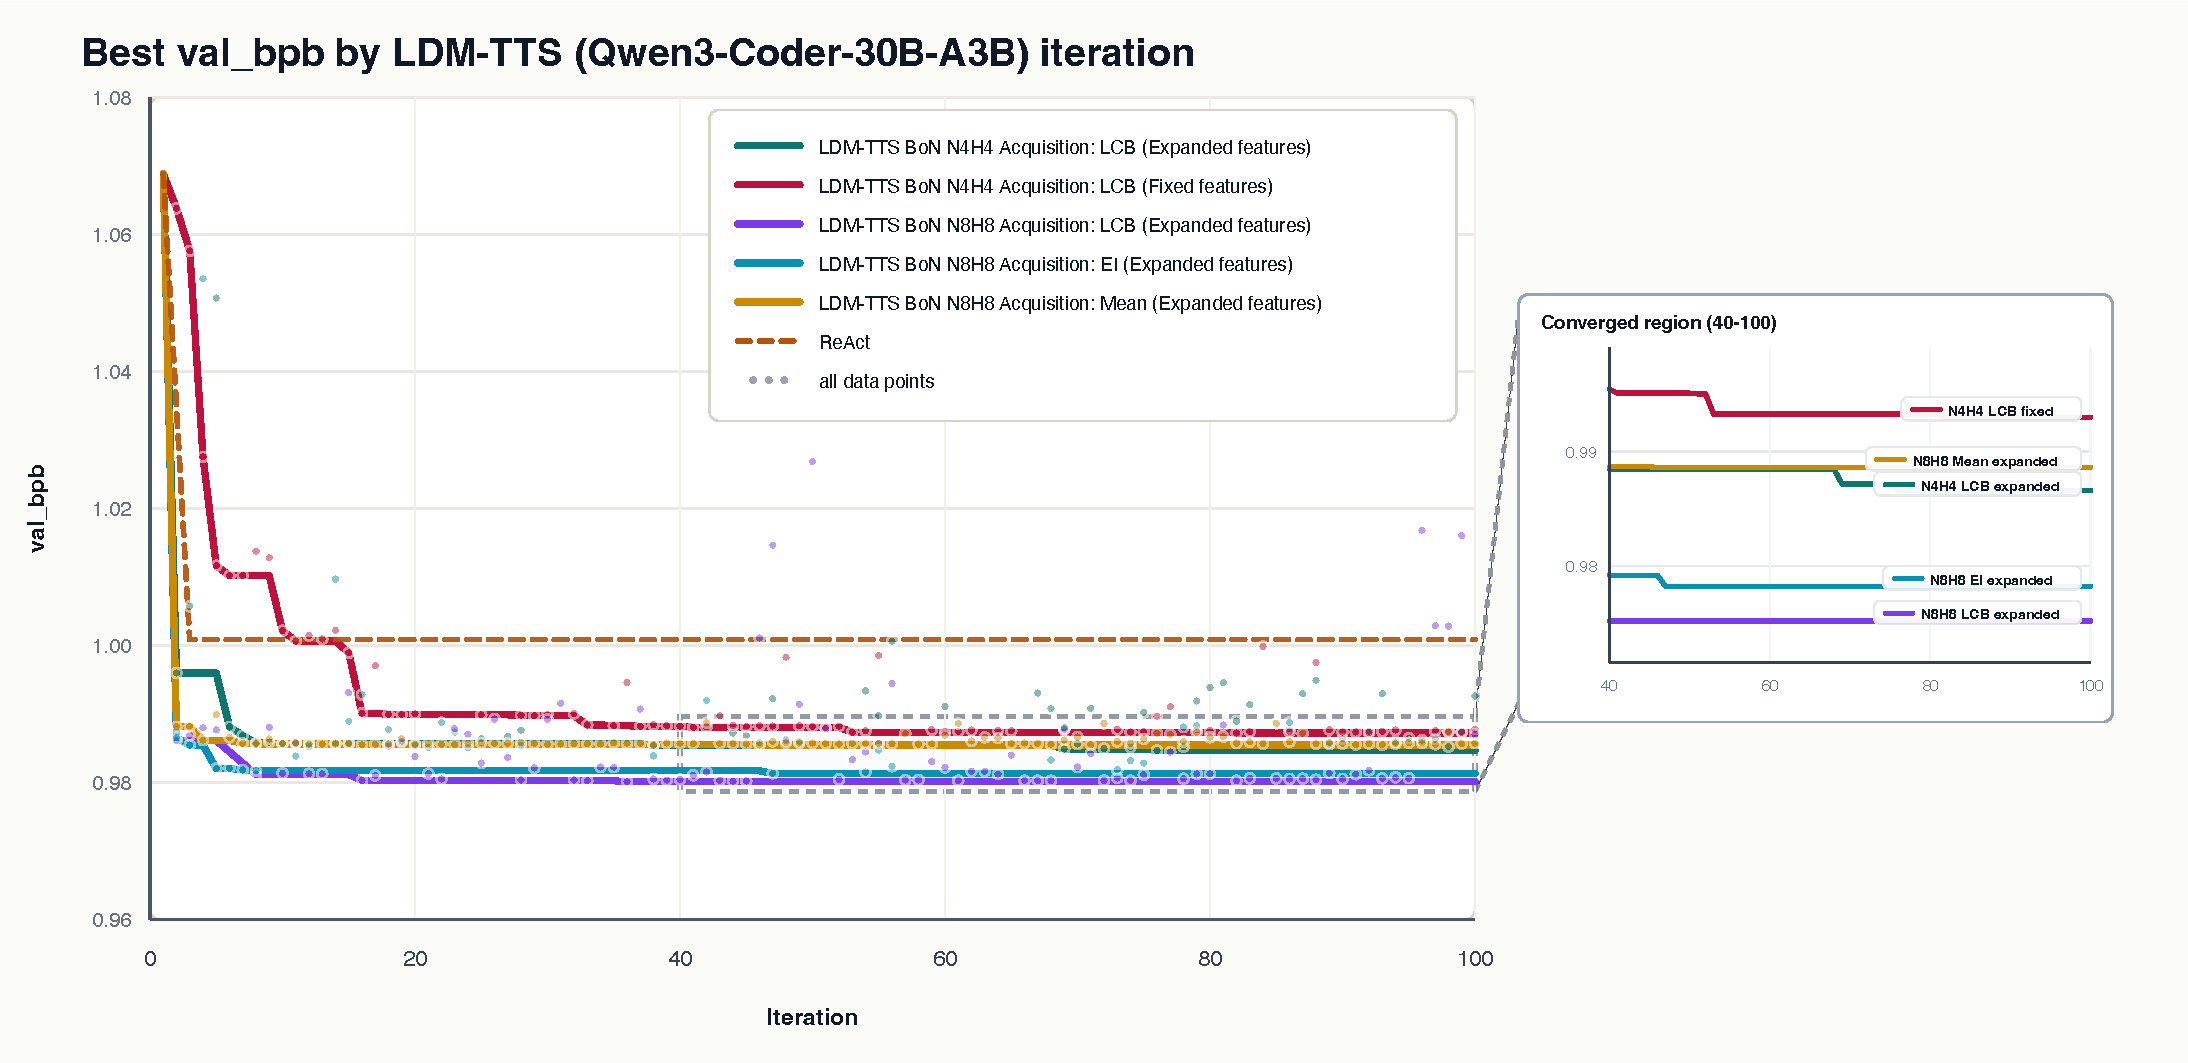
\includegraphics[width=\linewidth]{figure/val_bpb_multi_trial_best_by_iteration.pdf}
    \caption{\textbf{Test-time search ablation on \texttt{autoresearch}.} Best validation \texttt{val\_bpb} found up to iteration $t$ (lower is better). Solid curves are LDM-TTS variants; the dashed curve is a ReAct-style no-acquisition reference \citep{yao2022react}; gray points are all evaluated candidate programs. Each LDM-TTS variant is named \textsc{N$m$H$n$} for its inner budget, where $N$ is the number of candidate programs the LLM proposes and $H$ is the number of hypothesis/refinement branches each candidate is expanded into. }
    \label{fig:abl-autoresearch}
\end{figure}

Figure~\ref{fig:abl-autoresearch} gives three conclusions. First, \emph{increasing the test-time search budget helps}. The \textsc{N8H8} expanded-feature curve reaches the best plateau, while the lower-budget \textsc{N4H4} variants converge higher. Since the outer training budget is unchanged, this improvement comes from spending more cheap computation before each expensive evaluation. Second, \emph{dynamic feature expansion helps}, as \texttt{autoresearch} is not a fixed-dimensional hyperparameter problem. When the agent discovers a new mechanism, such as sparse memory or a new schedule family, the surrogate needs new coordinates on which to model it; fixed features compress those mechanisms into residual noise and produce weaker acquisition guidance. Third, \emph{the acquisition itself matters}. Posterior-mean search is competitive early because it exploits the most promising known direction, but it plateaus above EI and the uncertainty-aware acquisition. EI improves on mean-only selection by rewarding improvement over the incumbent, while the uncertainty-aware value performs best because it deliberately allocates part of the test-time budget to under-modelled program families. These results validate the central claim that the LLM is the semantic search engine, yet the calibrated acquisition is the value that makes additional test-time compute useful.

The same suite of test-time budget ablation sweeps was also conducted for the scientific design tasks detailed in \S\ref{sec:cs-molecule-results} and \S\ref{sec:cs-antibody-results}, with full results presented in Appendix~\ref{app:abl-molecule} and \ref{app:abl-antibody}, respectively. For molecular design, a clear trend emerges: larger search budgets yield more effective discovery. This pattern is weaker for antibody design, where the scaling effect is small in magnitude even though the optimum remains target-dependent across antigens; see Appendix~\ref{app:abl-antibody} for the per-target curves. The root cause is that the underlying large language model lacks specialised domain expertise, rendering its candidate proposals near-random. We further perform comparisons across different acquisition functions. Our results demonstrate that, given a sufficiently large search budget, well-chosen acquisition functions deliver consistent performance gains for both molecular and antibody design. Notably, the mean acquisition (a $0.5/0.5$ scalarisation of the Vina and activity objectives) outperforms EHVI under low search budgets for molecular design. The mechanism is bandwidth: EHVI is built on the strict Pareto frontier and therefore needs a large screening budget to be effective, while mean-style acquisitions collapse the two objectives into one scalar and at small budgets the per-step randomness from a thin screening budget partially substitutes for the missing Pareto signal.

\subsubsection{Hyperparameter sensitivity}

We next study the sensitivity of LDM to its two temperature parameters on the KRAS G12D molecular design task of \S\ref{sec:cs-molecule-results}. Here, the decoding parameter $\alpha$, which is the LLM sampling temperature $T_{\mathrm{LLM}}$, controls the diversity of LLM-generated SMILES candidates, while the acquisition temperature $\eta$ controls the strength of acquisition-guided selection. As $\eta\to0$ the policy collapses to the raw LLM reservoir and as $\eta\to\infty$ it reduces to acquisition-function argmax ($\eta=\infty$ in the experiments below).

\begin{figure*}[htbp]
    \centering
    \begin{subfigure}[t]{0.48\textwidth}
        \centering
        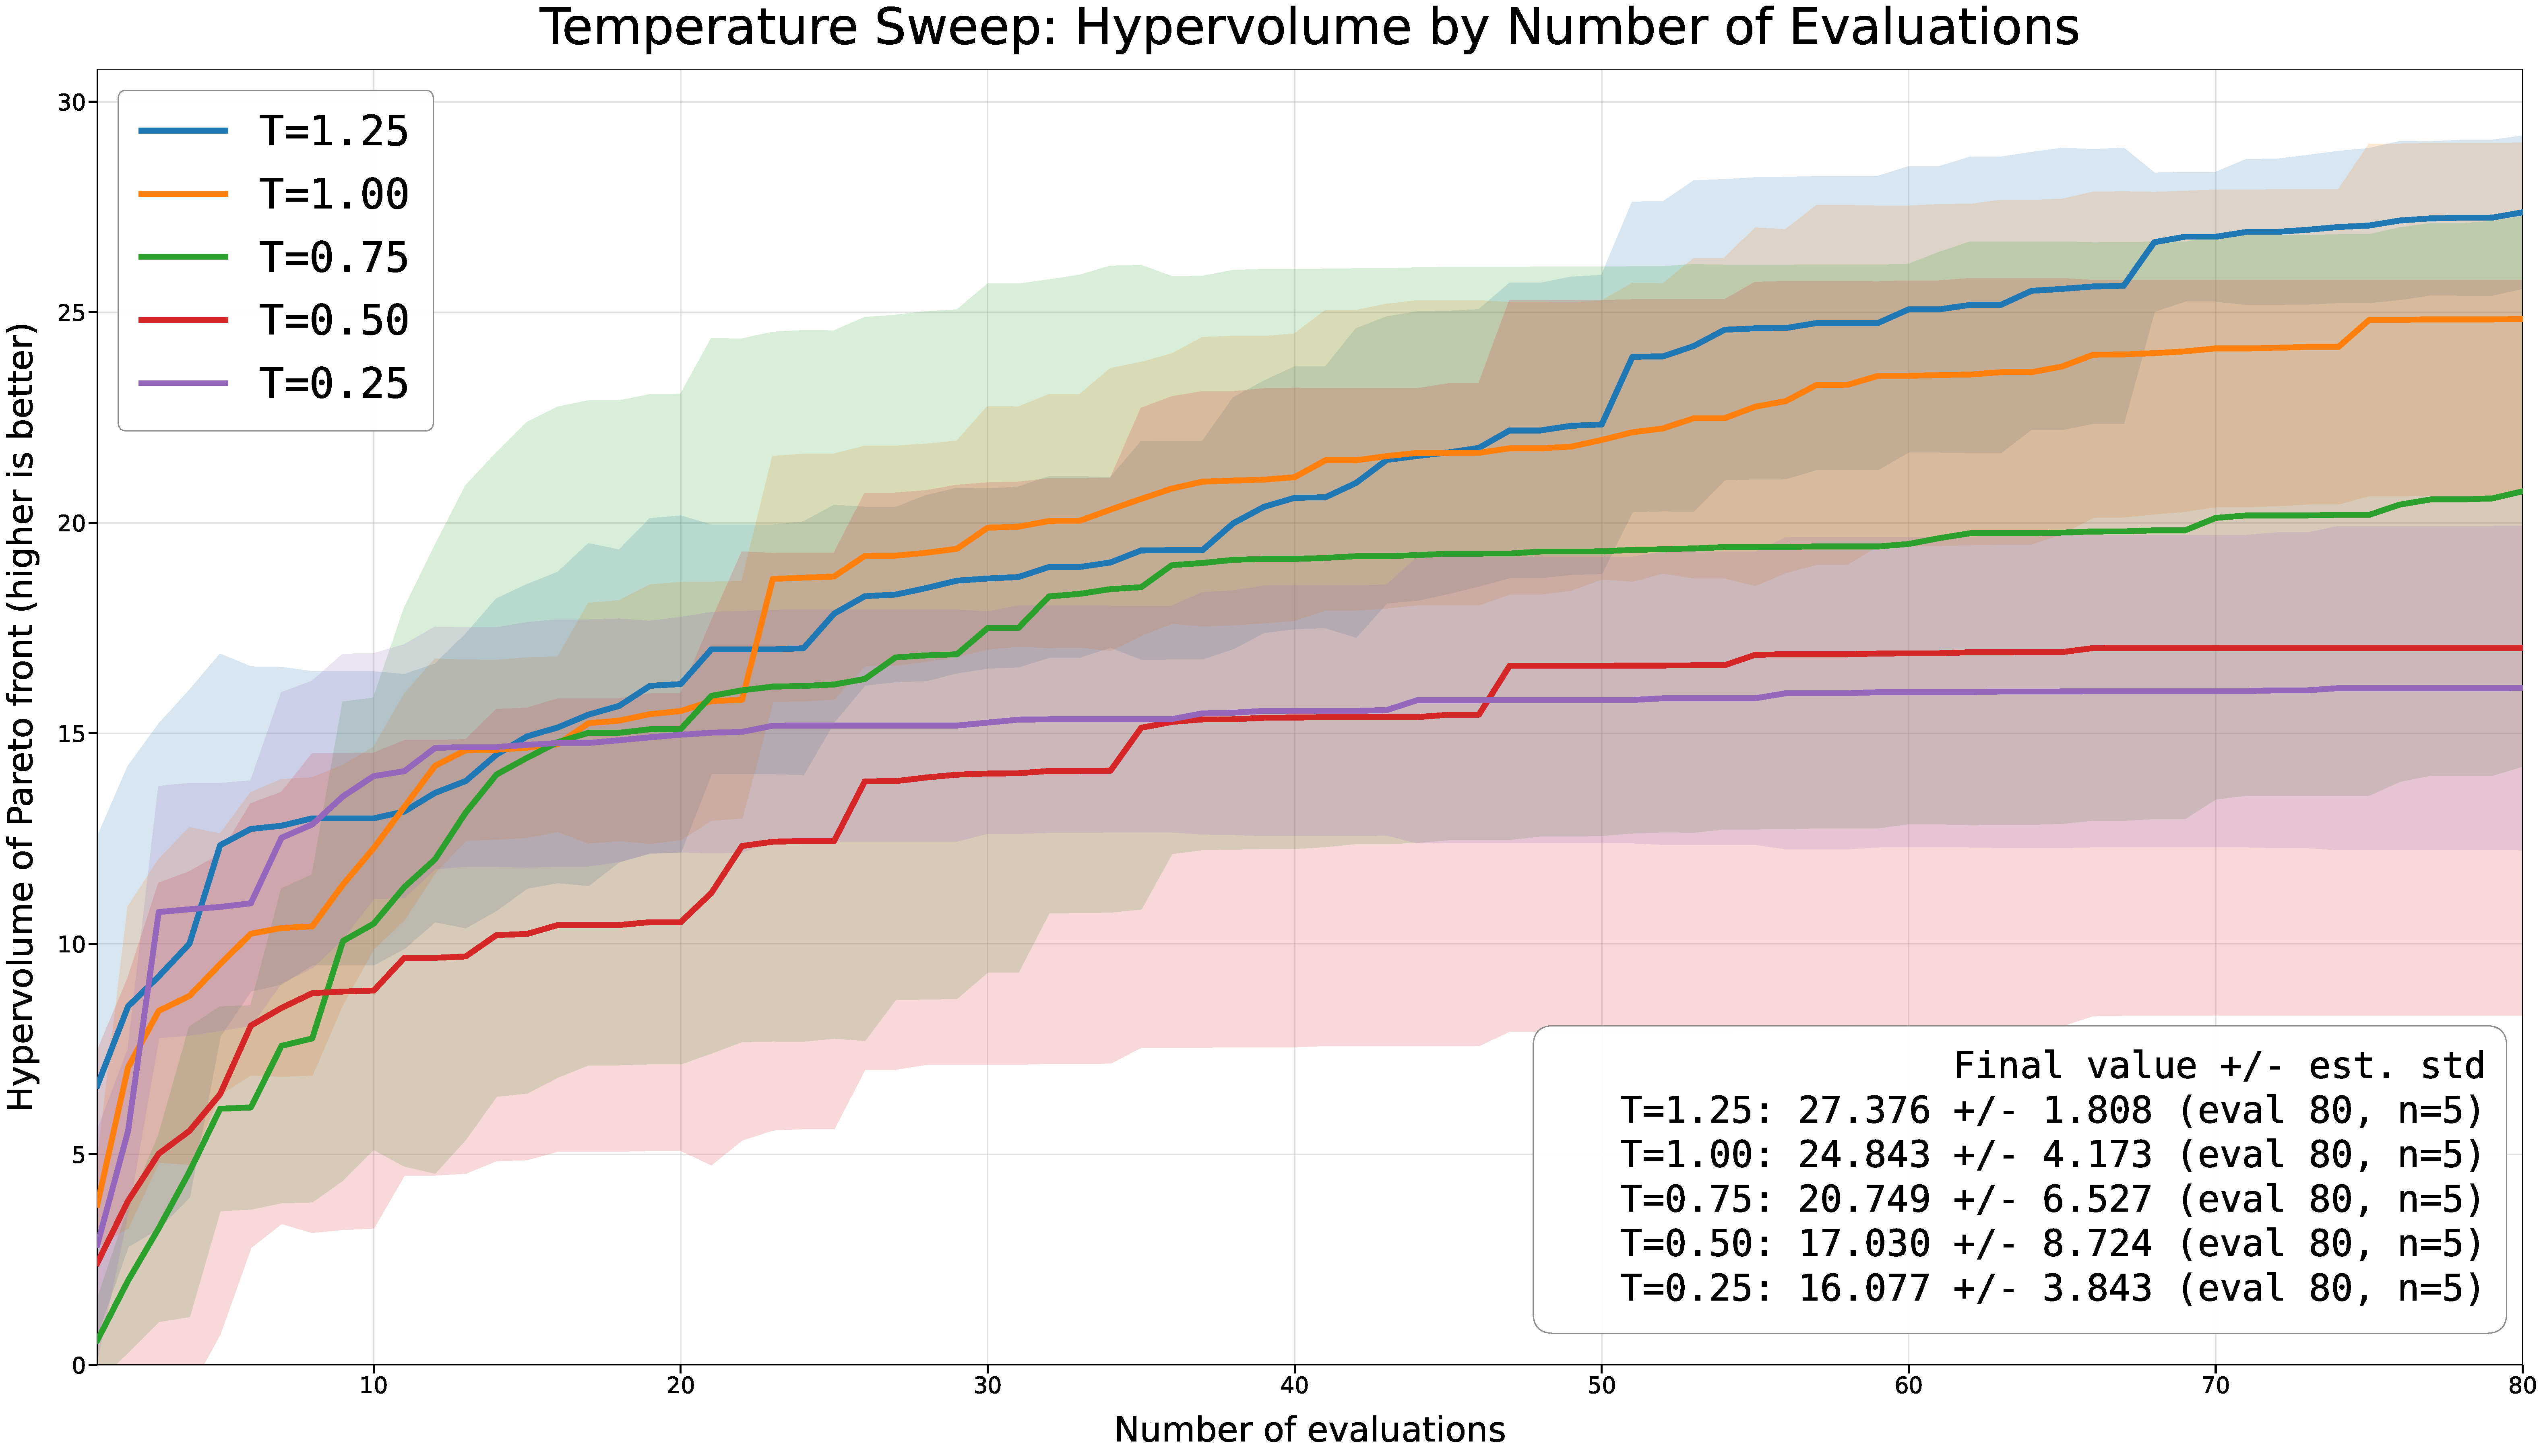
\includegraphics[width=\linewidth]{figure/ldm_molecule_temperature_sweep.pdf}
        \caption{Effect of LLM sampling temperature $T_{\mathrm{LLM}}$ with fixed acquisition temperature $\eta=1$.}
        \label{fig:molecule-temperature-ablation}
    \end{subfigure}
    \hfill
    \begin{subfigure}[t]{0.48\textwidth}
        \centering
        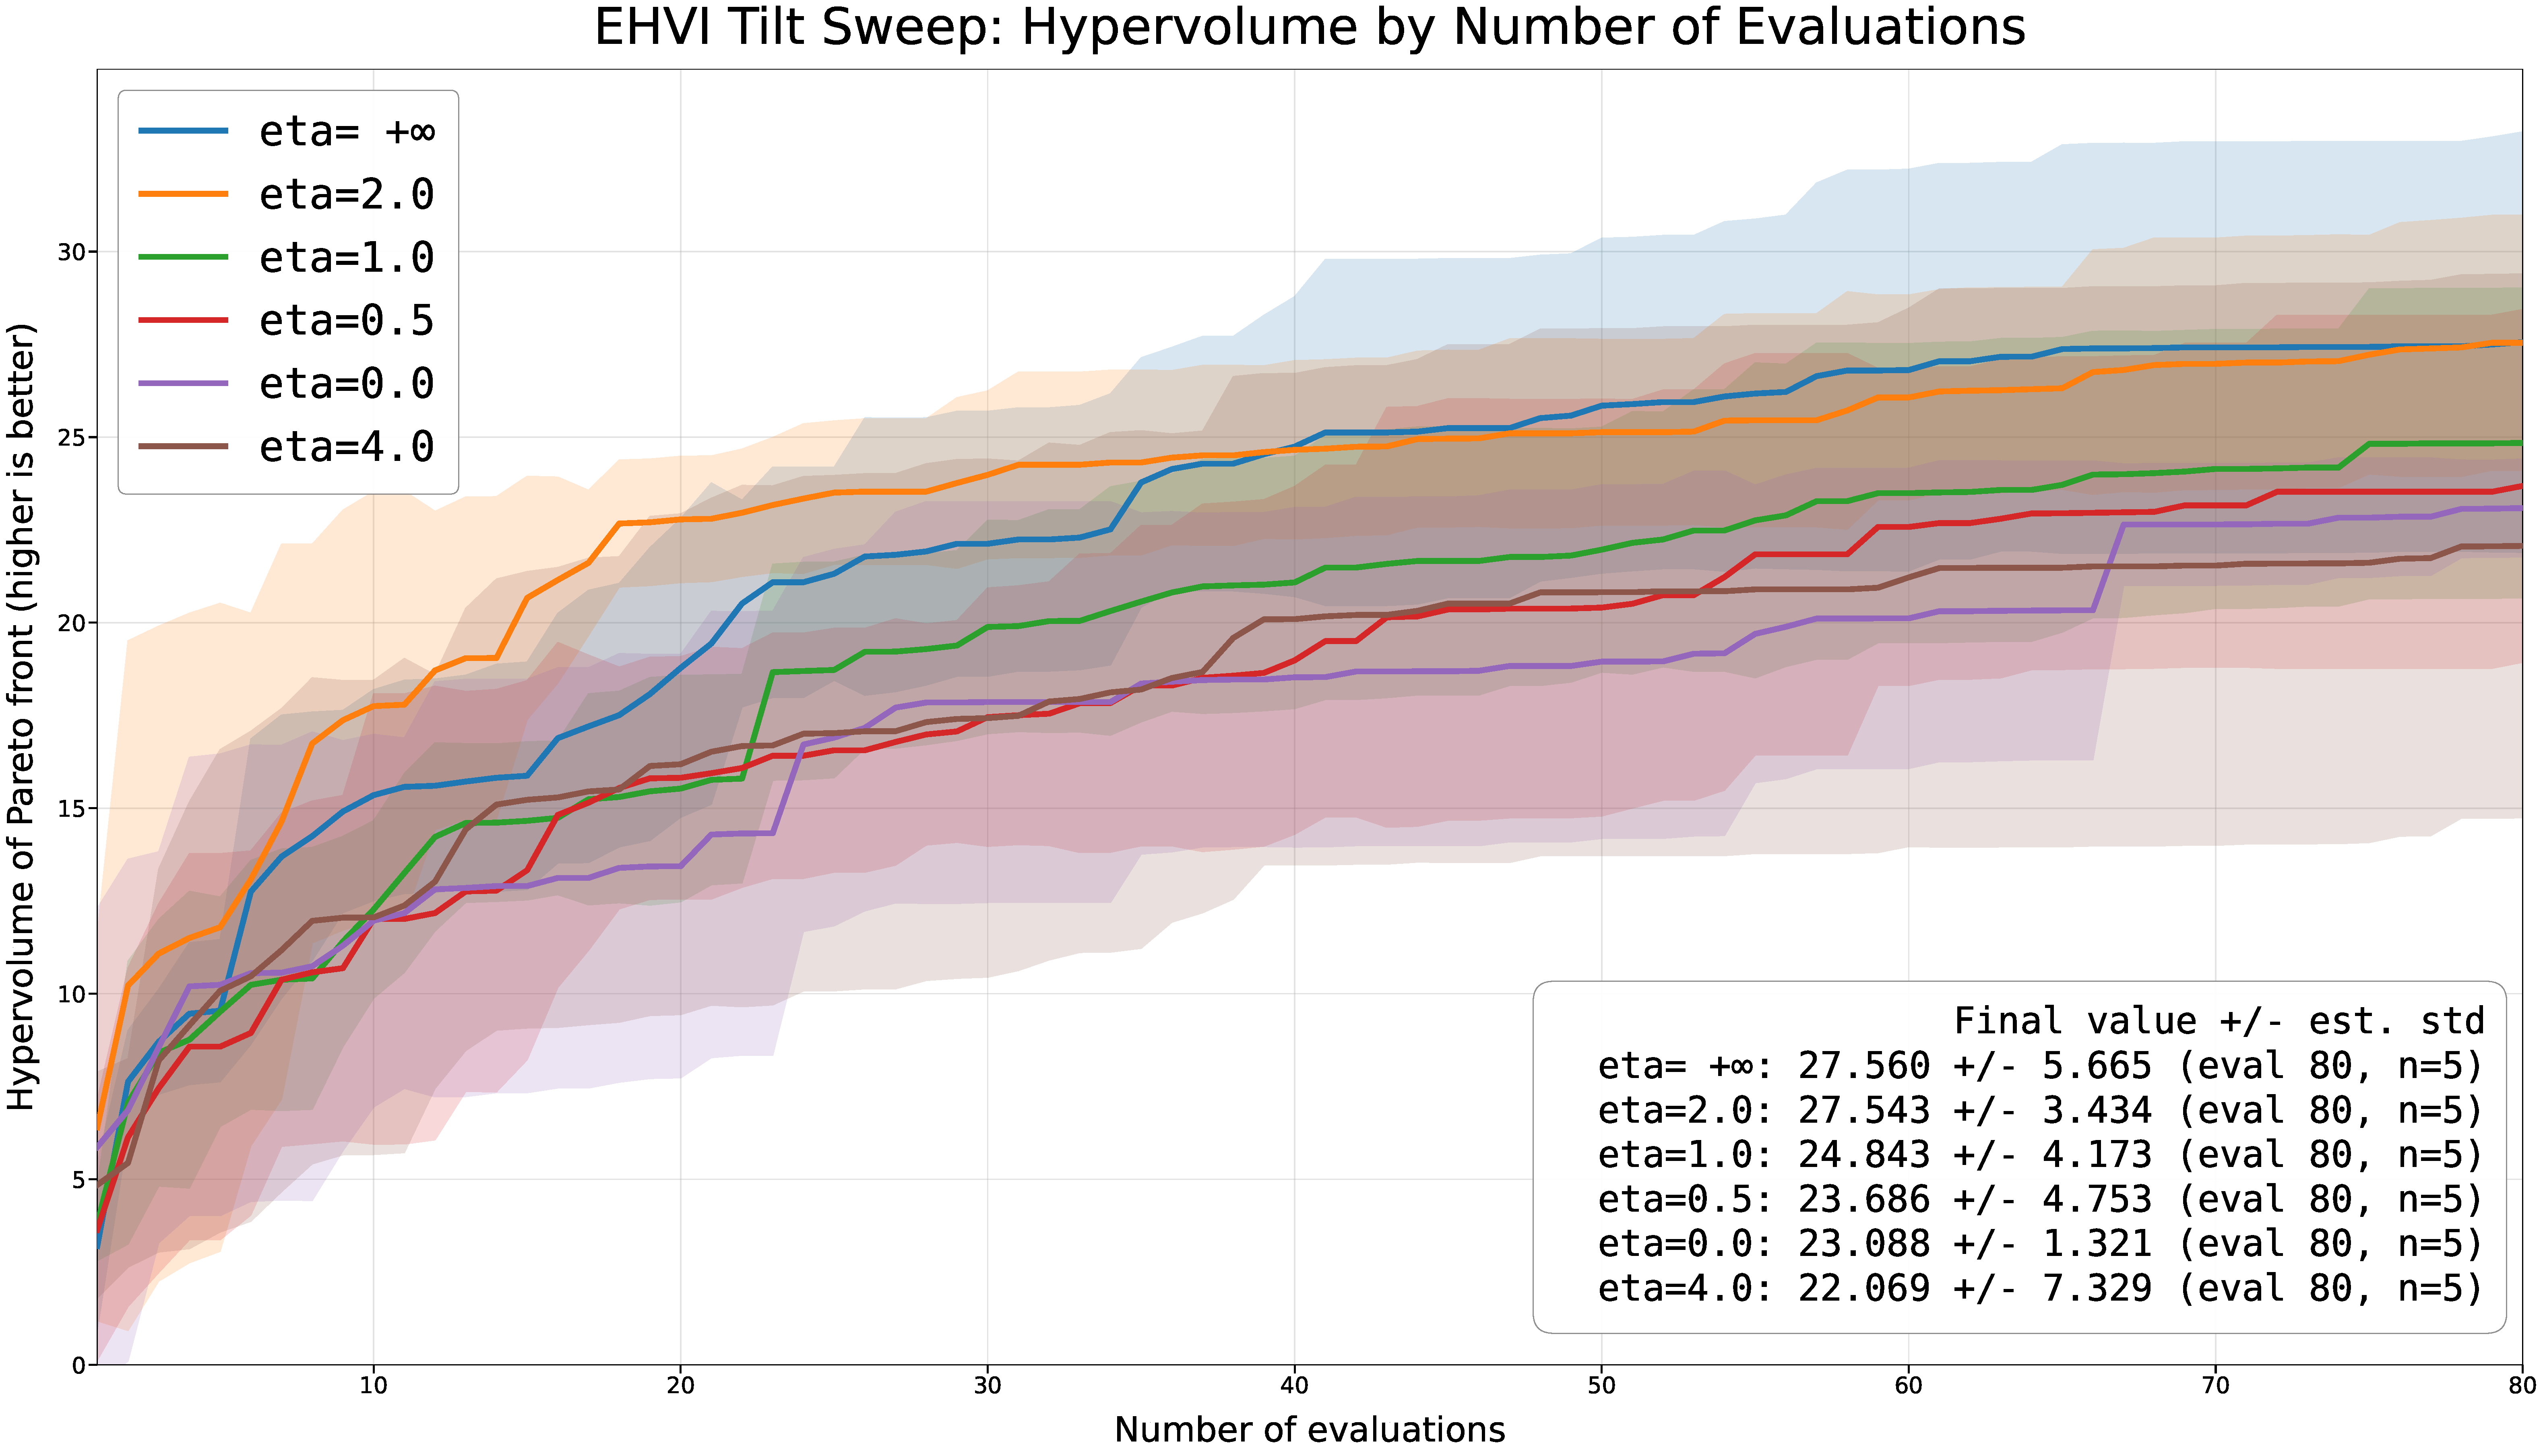
\includegraphics[width=\linewidth]{figure/ldm_molecule_eta_sweep.pdf}
        \caption{Effect of acquisition temperature $\eta$ with fixed LLM sampling temperature $T_{\mathrm{LLM}}=1$.}
        \label{fig:molecule-eta-ablation}
    \end{subfigure}

    \caption{\textbf{Hyperparameter ablations of LDM-TTS on molecular design.} Each curve reports the hypervolume of the Pareto front over the evaluation trajectory. Higher values indicate better multi-objective optimization performance.}
    \label{fig:molecule-temperature-eta-ablation}
\end{figure*}

For the LLM sampling temperature ablation, we fix $\eta=1$ and vary the LLM-decoding temperature $T_{\mathrm{LLM}}$ in $\{0.25, 0.5, 0.75, 1, 1.25\}$. As shown in Figure~\ref{fig:molecule-temperature-ablation}, increasing $T_{\mathrm{LLM}}$ generally improves the final optimization performance: the setting $T_{\mathrm{LLM}}=1.25$ achieves the highest final hypervolume, while lower temperatures degrade performance. For the acquisition temperature ablation, we fix $T_{\mathrm{LLM}}=1$ and vary $\eta\in\{0,0.5,1,\infty\}$. Figure~\ref{fig:molecule-eta-ablation} shows that increasing $\eta$ generally improves the final hypervolume. Overall, on molecular design both sufficient LLM exploration and effective acquisition guidance are necessary for LDM, with the acquisition tilt $\eta$ acting as the dominant driver of final Pareto-front expansion.

Antibody CDRH3 design (\S\ref{sec:cs-antibody-results}) yields distinct overall behaviour. The open-source LLM lacks biological sequence domain priors, generating nearly random candidate sequences across the vast search space. While policy-based LDM variants incorporate implicit acquisition-guided sampling to expand promising candidate regions, this diminishes the standalone impact of test-time acquisition reweighting. Therefore, global hyperparameter sweeps over sampling and acquisition temperatures reveal negligible performance sensitivity. This aligns with the core finding from \S\ref{sec:cs-antibody-results}: policy-mode LDM outperforms direct generation chiefly via built-in structural LLM priors instead of acquisition weighting. Full temperature ablation plots for antibody design are provided in Appendix~\ref{app:abl-hyper-ldm}.

% ============================================================
\subsection{Overall Discussion}
\label{sec:overall-discussion}

Collectively, the three case studies validate LDM as a general approach for model-based scientific discovery across distinct structured search domains, with consistent core conclusions emerging from all experimental setups.

First, combining calibrated Bayesian surrogate acquisition with LLM-driven inference-time search consistently outperforms standalone LLMs and vanilla Bayesian optimisation. LLMs supply native semantic generation over complex discrete spaces where BO cannot easily propose valid candidates, while Gaussian process surrogates deliver reliable uncertainty-aware value signals missing from uncalibrated LLM self-scoring. Neither component alone reproduces the full performance gains observed in the integrated LDM pipeline.

Second, the optimal LLM operating mode is domain-dependent, governed by the strength of the model’s pre-trained domain priors and the structure of the design space. For sparsely covered sequence spaces such as antibody CDRH3, policy-mode LLM search expands exploration coverage by defining local search zones. For domains with rich LLM pre-training data (code, SMILES), large-batch direct generation achieves superior Pareto/affinity improvements. The unified tilted distribution formulation accommodates both paradigms without modification to the underlying acquisition-guided optimisation logic.

Third, the three-way exploit–explore–discover trichotomy differentiates LDM from classic BO methods limited to two-way trade-offs. In all benchmarks, baseline systems lacking a generative reservoir eventually stagnate at fixed performance ceilings. LDM’s discovery mechanism breaks these plateaus by extending the set of candidate designs under evaluation whenever local optimisation yields no further gains, lifting the upper bound of achievable objective values over repeated iterations.

Fourth, the ablation and fine-tuning studies in \S\ref{sec:ablation-main} and \S\ref{sec:finetune-experiments} clarify why the framework works. Test-time search helps only when the additional inference-time compute is filtered by a calibrated, uncertainty-aware acquisition rather than by language plausibility, and the surrogate must track the search space as it evolves. When the LLM reservoir is itself weakly informative, as in antibody CDRH3 design, acquisition reweighting adds little beyond the policy's structural search. The fine-tuning results further show that the tilted search policy can be distilled into a single lightweight proposer, and that grounding distilled actions in surrogate value improves both same-domain and cross-task transfer. Together, these findings indicate that LDM's gains reflect a learnable discovery strategy rather than task-specific memorisation.

Finally, the empirical evidence reinforces this paper’s central framing: scientific design is an inverse decision problem rather than a forward prediction task. LDM constructs a learned surrogate landscape and searches within it for target-compliant structures, rather than only predicting properties from given inputs. The LLM acts as a flexible inference-time optimiser for Bayesian acquisition functions over semantically structured discrete spaces, not a replacement for principled uncertainty-aware optimisation. Remaining limitations include the cubic computational cost of exact Gaussian Processes at large evaluation budgets, and potential surrogate reward hacking. Even with these constraints, consistent performance improvements across program search, protein design and medicinal chemistry confirm that acquisition-guided LLM inference provides a broadly applicable foundation for autonomous closed-loop scientific discovery.
\section{Related Work}
\label{sec:related}

This section situates the LDMs within the broader literature on generative models, statistical optimisation, and their intersection for scientific discovery. The aim is not to provide an exhaustive survey, but a focused positioning of LDM within the key strands of related work that directly motivate its design and delineate its contributions. We structure the discussion in three parts. We first review the remarkable progress in LLMs, including their scaling laws, emergent reasoning capabilities, and post-training methods; we then highlight the limitations of pure generative models for discovery, particularly the lack of calibrated uncertainty and expensive, sparse reward signals. Next, we survey the statistical learning paradigm for scientific discovery, from multi-armed bandits to Bayesian optimisation (BO), and discuss its strengths and challenges in high-dimensional or open-ended, unrepresented scientific spaces. Finally, we examine the growing body of work on hybrid approaches that combine LLMs with BO, clarify the differences between LDM and the most closely related methods, and articulate the open problems our framework addresses.

\subsection{Large Language Models and Their Limitations in Scientific Discovery}

The early development of language models was marked by several landmark architectures, including the Transformer \citep{vaswaniAttentionAllYou2017}, GPT-1 \citep{radfordImprovingLanguageUnderstanding2018}, and BERT \citep{devlinBERTPretrainingDeep2019}. The past few years have witnessed transformative progress in large language models. Scaling laws \citep{kaplanScalingLawsNeural2020} have established a predictable correlation in LLMs' performance with the scale of model weights, data, and test-time compute. The remarkable success of GPT-3 \citep{brownLanguageModelsAre2020} further propelled research along the scaling direction. As models scale, they exhibit emergent abilities \citep{weiEmergentAbilitiesLarge2022} not present in smaller counterparts, including complex reasoning via chain-of-thought prompting \citep{weiChainofThoughtPromptingElicits2023,kojimaLargeLanguageModels2023}, in-context learning \citep{hanUnderstandingEmergentInContext2025}, and instruction following \citep{ouyangTrainingLanguageModels2022}. In addition, post-training methods, such as supervised fine-tuning (SFT) and reinforcement learning from human feedback (RLHF) \citep{ouyangTrainingLanguageModels2022}, can better adapt LLMs to downstream tasks and the users' preferences.

Since 2023, \emph{Test-time compute} has been a crucial development that pushes LLMs from language understanding to reasoners for complex problems, where the key insight is that the use of additional computation at inference time greatly improves output quality. Early research utilises verifiers \citep{cobbeTrainingVerifiersSolve2021, lightmanLetsVerifyStep2023} to guide reasoning to solve complex mathematical problems. Further, \emph{tree of thoughts} \citep{yao2023tree} performs deliberate search over intermediate reasoning states with self-evaluation. Self-Refine \citep{madaan2023selfrefine} iterates generate--critique--revise cycles. More generally, \citet{snell2025scaling} show that optimal allocation of test-time compute allows small models to outperform much larger models. The underlying search machinery, including UCT \citep{kocsis2006bandit} and the PUCT rule popularised by AlphaZero \citep{silver2017mastering}, has been applied to LLM decoding and training \citep{fengAlphazerolikeTreeSearchCan2024}. The combination of inference-time search with verifier-guided refinement underpins renowned systems such as OpenAI's o1 \citep{openaiOpenAIO1System2024} and DeepSeek-R1 \citep{deepseek-aiDeepSeekR1IncentivizingReasoning2025}. When cheap supervision is repeatedly available, \emph{reinforcement learning with verifiable rewards} (RLVR) \citep{deepseek-aiDeepSeekR1IncentivizingReasoning2025, shaoDeepSeekMathPushingLimits2024} has led to impressive results in mathematics, coding, and reasoning tasks. A unified tutorial perspective on these methods is provided by \citet{wangTutorialLLMReasoning2025}, and OpenR \citep{wang2024openr} further establishes a comprehensive technical framework.

Despite the significant progress of LLM reasoning, how LLMs engage in open-ended scientific discovery remains questionable. Studies show that LLMs are also poorly calibrated for scientific decisions---their internal confidence does not reliably reflect uncertainty about an external property \citep{guptaLLMsBayesianOptimization2025,kristiadiSoberLookLLMs2024}. Moreover, end-to-end execution benchmarks consistently show that frontier LLM agents cannot yet reliably discover novel, high-quality solutions: on ResearchClawBench the strongest autonomous agent scores only 21.5/50 across 40 real-paper-derived tasks \citep{xu2026researchclawbench}, and on PaperBench agents replicate ICML papers at 21.0\% against 41.4\% by PhD researchers \citep{starace2025paperbench}. Even at the ideation stage, novelty rankings that initially favour LLMs \citep{si2024novelideas} reverse once ideas are executed \citep{si2025executiongap}. LLM-generated ideas also exhibit narrow exploration, converging on the centroid of existing literature \citep{tang2026narrowexploration}. 

Therefore, scientific discovery essentially requires a novel paradigm of foundation models.  Crucially, the key challenge is not intrinsic LLM failures: when proposals are paired with automated evaluators and search, genuinely novel results are recovered \citep{novikov2025alphaevolve}. The bottleneck is the absence of a calibrated external value signal.  Test-time compute and reinforcement learning typically rely on cheap verifiers or reward models, such as ground-truth answers or trained networks from large data, to guide the search of reasoning steps. This is built upon access to rich feedback data or ground-truth answers, which, however, is usually scarce in scientific domains.

\subsection{Statistical Learning for Scientific Discovery}

A mature body of statistical learning approaches addresses the problem of optimising a black-box reward function with noisy evaluations. \emph{Multi-arm bandit} constitutes a representative framework conceptualising the exploration--exploitation trade-off \citep{lattimoreBanditAlgorithms2020}, where the upper confidence bound (UCB) \citep{auerUsingConfidenceBounds2002} provides a simple way to balance these competing objectives with sublinear regret guarantees. However, classical multi-arm bandit settings assume a finite set of arms, yet scientific design spaces are often effectively unbounded.

This challenge of unbounded space is then captured by the \emph{infinitely-armed bandit} \citep{berry1997bandit, wang2008infinitely} frameworks, where new arms must be discovered from a \emph{reservoir}. The performance in such settings is governed by the reservoir's tail of near-optimal arms, a quantity known as the \emph{discovery gap}. The LDM framework explicitly adopts this view, treating the LLM as an adaptive reservoir and analysing the discovery gap through a missing-mass argument \citep{mcallester2000convergence, berend2013concentration} in \S~\ref{sec:theory-main}. In comparison, LDM utilises an LLM as its reservoir, endowing the search process with broad scientific priors and rich semantic knowledge to inform candidate generation. In addition, the LLM’s context $\mathcal{C}_t$ encapsulates the full evaluation history, enabling in-context learning to synthesise insights from prior trials and propose progressively more effective candidate designs. The regret analysis in \S~\ref{sec:theory-main} decomposes the cost of search into a surrogate-estimation term and a reservoir-quality term, with the latter shrinking as more inference-time compute is spent.

Scientific discovery tasks are further constrained by costly evaluation procedures and limited computational budget. This demand motivates \emph{model-based} bandit variants that explicitly extract knowledge from evaluation history and make the most of such knowledge in decision making. To this end, \emph{Bayesian optimisation} (BO) \citep{mockusBayesMethodsSeeking1975,jonesEfficientGlobalOptimization1998,garnettBayesianOptimization2023} provides a powerful framework for such a variant that uses a probabilistic surrogate following the rigour of Bayesian inference, where typically a Gaussian process (GP) \citep{rasmussen2006gaussian} serves as the surrogate. The GP provides predictive mean and variance, which are combined into an \emph{acquisition function} that guides the selection of the next evaluation. For example, canonical implementations such as Efficient Global Optimisation (EGO) \citep{jonesEfficientGlobalOptimization1998} and GP-UCB \citep{srinivas2010gaussian} use expected improvement (EI) and UCB \citep{auerUsingConfidenceBounds2002} as their acquisition function, respectively. Theoretical analysis shows that GP-UCB enjoys sublinear cumulative regret in terms of the maximum information gain, a measure of how informative the observations are about the objective \citep{srinivas2010gaussian}. These theoretical guarantees make BO a principled tool for experimental design for scientific discovery \citep{yuEfficientPrincipledScientific2026}.

BO has been successfully applied across chemistry, materials science, and biology, often requiring domain-specific adaptations. Examples include the PHOENICS \citep{hasePhoenicsBayesianOptimizer2018} and Gryffin \citep{haseGryffinAlgorithmBayesian2021} frameworks for chemical discovery. Combinatorial BO frameworks such as AntBO \citep{khan2022antbo} have been developed to handle the discrete sequence space of CDRH3 loops for antibody design. Benchmarking studies across multiple materials domains \citep{liangBenchmarkingPerformanceBayesian2021} have compared different surrogate models and acquisition functions, while applications in chemical synthesis \citep{shieldsBayesianReactionOptimization2021} and material discovery \citep{shoyebraihanAcceleratingMaterialDiscovery2024} further demonstrate the versatility of BO. For a comprehensive overview of BO for chemical problems, see \citep{wuRaceBottomBayesian2024}. To search among discrete sequences (e.g., SMILES and proteins), methods such as BOSS (Bayesian Optimisation over String Spaces) \citep{mossBOSSBayesianOptimization2020} use string kernels to directly construct GPs over the string space. To handle molecule design, latent-space approaches combine variational autoencoders with BO, though they struggle with validity and out-of-distribution generation \citep{griffiths2020constrained}. More recent frameworks like COMBO \citep{dreczkowskiFrameworkBenchmarksCombinatorial2023} address combinatorial and mixed-variable optimisation. Multi-objective extensions (Expected Hypervolume Improvement) \citep{ponweiserMultiobjectiveOptimizationLimited2008, daulton2021parallel} handle the competing objectives common in drug discovery and materials science.

Despite these advances, pure statistical methods face fundamental challenges. First, they struggle to propose valid candidates in vast, unbounded spaces of practical scientific problems. Next, they cannot easily incorporate high-level semantic domain knowledge. Additionally, they are often unresponsive to user-specified design constraints or preferences. These limitations create a natural opportunity for complementarity with generative models, which can propose semantically meaningful candidates and be steered by domain knowledge. This brings us to the growing body of hybrid approaches that combine the strengths of LLMs and BO.

\subsection{Hybrid Approaches: LLM-Guided Discovery}

The recognition that LLMs and statistical learning offer complementary strengths has led to a growing body of hybrid methods. A high-level approach is OPRO \citep{yangLargeLanguageModels2024}, which uses an LLM as an optimizer by describing the task in natural language and iteratively generating solutions from a prompt containing a history of solution--score pairs. While powerful in prompt optimisation, OPRO lacks the calibrated uncertainty and principled exploration of a Bayesian surrogate.

Several works have integrated LLMs directly into the BO pipeline. LLAMBO \citep{liuLargeLanguageModels2024} uses LLMs for zero-shot warm-starting, surrogate modelling, and candidate sampling, showing gains in low-data hyperparameter optimisation regimes. BoChemian \citep{rankovicBoChemianLargeLanguage2023} and its extension \citep{rankovicLargeLanguageModels2025a} use LLM embeddings as features for BO over chemical reactions, demonstrating that fine-tuning LLMs with uncertainty-aware objectives can improve discovery rates. LABO \citep{chenLABOLLMAcceleratedBayesian2026} proposes a gating criterion to dynamically balance LLM predictions against experimental observations. Other works use LLMs to generate or refine kernels for GP surrogates \citep{suwandiAdaptiveKernelDesign2025}, handle natural language feedback \citep{kobalczykLILOBayesianOptimization2025}, or perform analog circuit design \citep{yinADOLLMAnalogDesign2024,chenLLMEnhancedBayesianOptimization2024}. The LLM-as-warm-start paradigm, where the LLM suggests the initial candidates or a search region, is also explored in \citep{ramosBayesianOptimizationCatalysis2025, yinADOLLMAnalogDesign2024}. In catalysis, \citet{ramosBayesianOptimizationCatalysis2025} use frozen LLMs for in-context learning to enable BO without feature engineering, demonstrating the potential of LLMs to operate directly in language space.

Despite various attempts to combine the advantages of LLMs and BO, some recent studies have challenged their solidity. A sobering perspective is provided by \citet{guptaLLMsBayesianOptimization2025}, who find that current LLMs show no sensitivity to experimental feedback in BO tasks, and classical methods such as linear bandits and GP optimisation consistently outperform LLM agents. Similarly, \citet{kristiadiSoberLookLLMs2024} take a dispassionate stance, concluding that uncertainty taken directly from point-estimated LLMs is unreliable, and that LLMs are useful for BO over molecules primarily only when they serve as fixed feature extractors for principled GP surrogates and are pretrained or finetuned on domain-specific data. These critiques directly motivate LDM's design: we retain an explicit calibrated posterior (the GP surrogate) and use the LLM only as a candidate reservoir.

Another closely related work to LDM is dLLM \citep{yuan2026diffusion}, which for \emph{offline} black-box optimisation runs a masked-diffusion tree search where leaf candidates are scored by expected improvement under a GP fitted to an offline dataset. In contrast, LDM targets the standard \emph{online} recurrent loop with sequential, expensive evaluations. The core is that LDM must raise designs that are valuable not only for the current trial but also for gaining knowledge for the future.

In summary, LLMs provide powerful generative priors but lack calibration and robust optimisation; meanwhile, statistical methods provide principled, uncertainty-aware search but struggle to propose candidates in semantic, combinatorial spaces. LDM bridges this gap by making the acquisition function the value signal of an LLM-driven inference-time search, creating a principled, model-based framework for scientific discovery.

\section{Conclusion}
\label{sec:conclusion}

The core challenge of scientific discovery lies in searching for optimal solutions within vast, structured and open-ended design spaces under a limited budget of costly evaluations. Existing paradigms exhibit complementary limitations: large language models (LLMs) possess strong structured generative capabilities and domain priors, but cannot reliably estimate the true value of external objectives or their associated uncertainty. Bayesian optimisation, by contrast, delivers uncertainty-aware experimental decisions from sparse observations, yet struggles to autonomously propose valid candidates in complex discrete spaces. This work presents the Large Discovery Model (LDM), an experiment-grounded recurrent architecture that deeply couples the generative prior of LLMs with the value signal from a Gaussian process surrogate. Framing scientific design as a sequential inverse decision problem under an evaluation budget, LDM operates a closed loop of generation, evaluation and update that simultaneously expands the search frontier and allocates experimental resources precisely.

At the theoretical and algorithmic level, LDM establishes a KL-regularised, acquisition-guided optimisation framework and derives a closed-form acquisition-tilted optimal search distribution. This formulation extends the classical dichotomy between exploitation and exploration into a tripartite scientific search regime of exploitation, exploration and discovery, unifying the generative prior and empirical value signal within a single mathematical framework. We further provide a complete regret decomposition that explicitly delineates the performance boundaries of generative coverage gap, surrogate fitting error and sampling strategy suboptimality. Algorithmically, the framework supports two candidate generation paradigms, direct generation and indirect parameterisation, and is complemented by a decomposed feedback mechanism to guide targeted iterative refinement, making it adaptable to design spaces of varying structure. Building on this core, we introduce a post-training amortisation scheme: through reasoning-augmented supervised fine-tuning, the high-budget test-time search policy is amortised into the model weights, substantially reducing inference-time computational cost while preserving search quality.

Empirical evaluation across three heterogeneous domains, including the auto-research scenario of neural-network training programme, antibody CDRH3 sequence design, and multi-objective molecular optimisation, systematically validates the generality of the LDM framework and its core findings. First, the structured generative capacity of LLMs and the uncertainty calibration of Bayesian surrogates exhibit strong complementarity, with their integrated performance consistently outperforming both LLM-only and BO-only baselines. Second, the discovery mechanism is central to breaking performance plateaus: purely local optimisation converges rapidly to local optima, whereas expansion of the search frontier continuously lifts the attainable performance ceiling. Third, both test-time compute scaling and post-training fine-tuning reliably improve search efficiency, and the optimal generation paradigm correlates with the strength of domain priors. Fine-tuning experiments further demonstrate stable gains across cross-target and cross-task transfer, indicating that the model learns generalisable discovery decision logic rather than task-specific memorisation.

Nevertheless, the current framework is subject to several constraints and limitations. The Gaussian process surrogate incurs cubic computational complexity in the number of observations, limiting its scalability under large experimental budgets. Test-time search relies on batch candidate sampling, which entails substantial LLM inference overhead. The kernel functions and feature representations of the surrogate still require manual customisation per domain, resulting in limited automation for cross-domain transfer. Additionally, framework performance is bounded by the coverage of the LLM’s pretrained domain knowledge; in domains with weak priors, it is difficult to achieve substantial superiority over specialised methods. Finally, the current closed loop is updated solely based on in-process experimental observations, and has not yet systematically incorporated external existing knowledge and data, leaving a large body of unknown knowns unutilised in the search process.

For future work, a core direction is to address the utilisation of unknown knowns. We will introduce memory retrieval mechanisms and federated discovery frameworks to incorporate external knowledge bases, published experimental results and data from parallel exploration processes into the search closed loop. Combined with techniques such as sparse Gaussian processes \citep{snelsonSparseGaussianProcesses2005, titsiasVariationalLearningInducing2009}, this will simultaneously resolve the dual challenges of limited context capacity and high computational complexity as observational data scales. Building on this, we will explore end-to-end surrogate specification, in which the LLM autonomously learns kernel functions and prior settings for the surrogate, eliminating manual adaptation across domains. We will also advance discovery-oriented post-training paradigms, exploring more sophisticated training paths such as preference learning and reinforcement learning to further internalise the acquisition-tilted decision logic into the model’s generative distribution. This would endow the model with native capability to balance exploitation, exploration and discovery, ultimately enabling more efficient open-ended scientific discovery.


\bibliographystyle{plainnat}
\bibliography{references}

\newpage
\appendix

% ============================================================
\section{Detailed Proofs}
\label{sec:theory}
% ============================================================

We give the full proof of Proposition~\ref{prop:gibbs}, Lemma~\ref{lem:gibbs-near-ucb} and Theorem~\ref{thm:regret}.
\subsection{Proof of Proposition~\ref{prop:gibbs}}
\label{prop_proof}
\begin{proof}
Write $J(q)=\E_{x\sim q}[\acq_t]-\tfrac1\eta\KL(q\|p_{\theta,\alpha})$. For any $q$,
\[
J(q)=\sum_x q(x)\acq_t(x)-\tfrac1\eta\sum_x q(x)\log\frac{q(x)}{p_{\theta,\alpha}(x)}
=-\tfrac1\eta\sum_x q(x)\log\frac{q(x)}{p_{\theta,\alpha}(x)e^{\eta\acq_t(x)}}.
\]
Define $\pi_t(x)\propto p_{\theta,\alpha}(x)e^{\eta\acq_t(x)}$ with normaliser $Z_t$. Substituting,
\[
J(q)=-\tfrac1\eta\,\KL(q\|\pi_t)+\tfrac1\eta\log Z_t\ \le\ \tfrac1\eta\log Z_t,
\]
with equality iff $q=\pi_t$, since $\KL(q\|\pi_t)\ge 0$ with equality iff $q=\pi_t$. As
$p_{\theta,\alpha}\propto p_\theta^{\alpha}$, the normalising constants combine into $Z_t$, giving
\eqref{eq:core}.
\end{proof}

\subsection{Proof of Lemma~\ref{lem:gibbs-near-ucb}}
\label{app:gibbs-lemma}

Fix a round $t$ and condition on the history $\C_t$. Under this conditioning, the effective
reservoir support $A_t$, the inference-configured proposal $p_{\theta,\alpha}(\cdot\mid\C_t)$, and
the acquisition function $\acq_t(x)=\mu_t(x)+\sqrt{\beta_t}\sigma_t(x)$ are fixed. Let
\[
Z_t=\sum_{u\in A_t}\exp\{\eta\,\acq_t(u)\}\,p_{\theta,\alpha}(u\mid\C_t)
\]
be the normalising constant of \eqref{eq:theory-pi}. For a tolerance $\zeta_t\ge0$, write
\[
U=U_t(\zeta_t)
=
\{x\in A_t:\acq_t(x)\ge a_{t,A}^\star-\zeta_t\}.
\]
Every $u\in U$ has acquisition at least $a_{t,A}^\star-\zeta_t$. Hence the contribution of $U$ alone gives the
lower bound
\begin{align}
Z_t
&=
\sum_{u\in A_t}\exp\{\eta\,\acq_t(u)\}\,p_{\theta,\alpha}(u\mid\C_t) \notag\\
&\ge
\sum_{u\in U}\exp\{\eta\,\acq_t(u)\}\,p_{\theta,\alpha}(u\mid\C_t) \notag\\
&\ge
\exp\{\eta(a_{t,A}^\star-\zeta_t)\}\,p_{\theta,\alpha}(U\mid\C_t) \notag\\
&=
\kappa_t(\zeta_t)\exp\{\eta(a_{t,A}^\star-\zeta_t)\}.
\label{eq:zt-lower}
\end{align}

Now fix $z\ge0$ and define the bad event
\[
B_z=
\{x\in A_t:a_{t,A}^\star-\acq_t(x)>\zeta_t+z\}.
\]
For every $x\in B_z$,
\[
\acq_t(x)<a_{t,A}^\star-\zeta_t-z.
\]
Therefore,
\begin{align}
\Prob(x_t\in B_z\mid\C_t)
&=
\pi_t(B_z) \notag\\
&=
\frac{\sum_{x\in B_z}\exp\{\eta\,\acq_t(x)\}\,p_{\theta,\alpha}(x\mid\C_t)}{Z_t} \notag\\
&\le
\frac{\exp\{\eta(a_{t,A}^\star-\zeta_t-z)\}\,p_{\theta,\alpha}(B_z\mid\C_t)}
{\kappa_t(\zeta_t)\exp\{\eta(a_{t,A}^\star-\zeta_t)\}} \notag\\
&\le
\frac{\exp\{-\eta z\}}{\kappa_t(\zeta_t)},
\label{eq:gibbs-tail}
\end{align}
where the first inequality uses \eqref{eq:zt-lower}, and the second uses $p_{\theta,\alpha}(B_z\mid\C_t)\le1$. This proves the
tail form
\[
\Prob\left(
a_{t,A}^\star-\acq_t(x_t)>\zeta_t+z
\mid
\C_t
\right)
\le
\frac{e^{-\eta z}}{\kappa_t(\zeta_t)}.
\]

To obtain the high-probability statement, take
\[
z=\frac1\eta\log\frac1{\rho_t\kappa_t(\zeta_t)}.
\]
Since $\rho_t\in(0,1)$ and $\kappa_t(\zeta_t)\le1$, this $z$ is non-negative. Substitution into
\eqref{eq:gibbs-tail} gives an upper bound of $\rho_t$ on the bad event, so with conditional probability at
least $1-\rho_t$,
\[
a_{t,A}^\star-\acq_t(x_t)
\le
\zeta_t+\frac1\eta\log\frac1{\rho_t\kappa_t(\zeta_t)}.
\]
This proves Lemma~\ref{lem:gibbs-near-ucb}.

\subsection{Proof of Theorem~\ref{thm:regret}}
\label{app:main-proof}

The proof decomposes regret into a discovery term and an optimisation term, then controls the optimisation term
using UCB calibration and Lemma~\ref{lem:gibbs-near-ucb}.

As stated earlier, we can control the simple regret by analysing the upper bound of the cumulative regret, which can be decomposed by the discovery gap and optimisation regret as below.
\begin{equation}
\regret_t
=
\underbrace{R(x^\star)-R_{t,A}^\star}_{\regret_t^{\rm disc}}
+
\underbrace{R_{t,A}^\star-R(x_t)}_{\regret_t^{\rm opt}}.
\label{eq:disc-opt-decomp}
\end{equation}


We begin with bounding the discovery gap. By Assumption~\ref{ass:coverage}, for every $x\in A_t$,
\[
R(x^\star)-R(x)
\le
L\,\mathrm d_\X(x,x^\star)^\chi.
\]
Taking the infimum over $x\in A_t$ gives
\begin{align}
\regret_t^{\rm disc}
&=
R(x^\star)-\sup_{x\in A_t}R(x) \notag\\
&=
\inf_{x\in A_t}\{R(x^\star)-R(x)\} \notag\\
&\le
L\inf_{x\in A_t}\mathrm d_\X(x,x^\star)^\chi \notag\\
&=
L\left(\inf_{x\in A_t}\mathrm d_\X(x,x^\star)\right)^\chi \notag\\
&=
L(r_t^{\rm cov})^\chi.
\label{eq:disc-gap-bound}
\end{align}
Thus, the discovery price is exactly controlled by the current reservoir coverage radius.

Next, we form the simultaneous sampling event. For each $t$, apply Lemma~\ref{lem:gibbs-near-ucb} with failure probability $\rho_t$. Define
\[
\xi_t
=
\zeta_t+\frac1\eta\log\frac1{\rho_t\kappa_t(\zeta_t)}.
\]
The lemma gives, conditionally on $\C_t$,
\[
\Prob(a_{t,A}^\star-\acq_t(x_t)\le \xi_t\mid \C_t)\ge1-\rho_t.
\]
Equivalently, the conditional failure probability is at most $\rho_t$. Iterating this bound over
$t=1,\ldots,T$ and applying a union bound yields an event $\mathcal E_{\rm samp}$ such that
\[
\Prob(\mathcal E_{\rm samp})\ge 1-\sum_{t=1}^T\rho_t\ge1-\delta_{\rm samp},
\]
and on $\mathcal E_{\rm samp}$,
\begin{equation}
a_{t,A}^\star-\acq_t(x_t)\le \xi_t
\qquad\text{for all }t\le T.
\label{eq:sampling-event}
\end{equation}

As such, we can bound the optimisation term on the good event. Let $\mathcal E_{\rm gp}$ be the event in Assumption~\ref{ass:ucb-calibration}. On this event, for every
$x\in\X$ and $t\le T$,
\begin{equation}
\begin{aligned}
R(x)\le \acq_t(x),
\qquad
R(x)\ge \mu_t(x)-\sqrt{\beta_t}\sigma_t(x).
\end{aligned}
\label{eq:ucb-two-sided}
\end{equation}
On $\mathcal E_{\rm gp}\cap\mathcal E_{\rm samp}$,
\begin{align}
R_{t,A}^\star
&=
\sup_{x\in A_t}R(x) \notag\\
&\le
\sup_{x\in A_t}\acq_t(x) \notag\\
&=
a_{t,A}^\star \notag\\
&\le
\acq_t(x_t)+\xi_t,
\label{eq:best-in-a-upper}
\end{align}
where the first inequality uses UCB optimism and the last inequality uses \eqref{eq:sampling-event}. Therefore
\[
\regret_t^{\rm opt}
=
R_{t,A}^\star-R(x_t)
\le
\acq_t(x_t)-R(x_t)+\xi_t.
\]
Using the lower side of \eqref{eq:ucb-two-sided} at the sampled point $x_t$,
\begin{align}
\acq_t(x_t)-R(x_t)
&=
\mu_t(x_t)+\sqrt{\beta_t}\sigma_t(x_t)-R(x_t) \notag\\
&\le
2\sqrt{\beta_t}\sigma_t(x_t).
\end{align}
Hence
\begin{equation}
\regret_t^{\rm opt}
\le
2\sqrt{\beta_t}\sigma_t(x_t)+\xi_t.
\label{eq:opt-gap-bound}
\end{equation}

Combining \eqref{eq:disc-opt-decomp}, \eqref{eq:disc-gap-bound}, and \eqref{eq:opt-gap-bound}, on $\mathcal E_{\rm gp}\cap\mathcal E_{\rm samp}$ we have, for every $t\le T$,
\[
\regret_t
\le
L(r_t^{\rm cov})^\chi
+
2\sqrt{\beta_t}\sigma_t(x_t)
+
\xi_t.
\]
Summing over $t$ and using the monotonicity $\beta_t\le\beta_T$,
\begin{equation}
\sum_{t=1}^T\regret_t
\le
L\sum_{t=1}^T(r_t^{\rm cov})^\chi
+
2\sqrt{\beta_T}\sum_{t=1}^T\sigma_t(x_t)
+
\sum_{t=1}^T\xi_t.
\label{eq:sum-delta-before-info}
\end{equation}

By the standard information-gain variance bound for GP-UCB,
\[
\sum_{t=1}^T\sigma_t^2(x_t)
\le
C_\lambda\gamma_T,
\qquad
C_\lambda=\frac{2}{\log(1+\lambda^{-1})}.
\]
Therefore, by Cauchy--Schwarz,
\begin{equation}
\sum_{t=1}^T\sigma_t(x_t)
\le
\sqrt{T\sum_{t=1}^T\sigma_t^2(x_t)}
\le
\sqrt{T C_\lambda\gamma_T}.
\label{eq:variance-sum}
\end{equation}
Substituting \eqref{eq:variance-sum} into \eqref{eq:sum-delta-before-info} gives
\[
\sum_{t=1}^T\regret_t
\le
L\sum_{t=1}^T(r_t^{\rm cov})^\chi
+
2\sqrt{T C_\lambda\beta_T\gamma_T}
+
\sum_{t=1}^T\xi_t.
\]
Finally, substituting the definition of $\xi_t$,
\[
\frac{1}{T}\sum_{t=1}^T \regret_t
\le
\frac{L}{T}\sum_{t=1}^T(r_t^{\rm cov})^\chi
+
2\sqrt{\frac{C_\lambda\beta_T\gamma_T}{T}}
+
\frac1T\sum_{t=1}^T
\left[
\zeta_t+
\frac1\eta\log\frac1{\rho_t\kappa_t(\zeta_t)}
\right].
\]

Assumption~\ref{ass:ucb-calibration} gives $\Prob(\mathcal E_{\rm gp})\ge1-\delta_{\rm gp}$, and the sampling
argument gives $\Prob(\mathcal E_{\rm samp})\ge1-\delta_{\rm samp}$. A final union bound gives
\[
\Prob(\mathcal E_{\rm gp}\cap\mathcal E_{\rm samp})
\ge
1-\delta_{\rm gp}-\delta_{\rm samp}.
\]
This completes the proof of Theorem~\ref{thm:regret}.

\section{Technical Implementation Details}
\label{sec:impl-details}

This appendix elaborates on the core algorithmic and implementation details of the LDM framework, covering Gaussian process surrogate modelling, acquisition function design and batch sampling schemes. All implementations strictly follow the acquisition-tilted search framework presented in the main text, and only expand on the specific execution logic for surrogate model training and sampling.

\subsection{Gaussian Process Surrogate}
\label{sec:llm-bo}

LDM employs a Gaussian Process (GP) as the probabilistic surrogate model. It fits the posterior distribution of the black-box reward function from historical experimental observations, and outputs calibrated predictive means and epistemic uncertainty to provide quantitative inputs for acquisition function computation.

\subsubsection{Prior Specification}
Let $\mathcal{X}$ denote the design space, $R(x)$ the true black-box reward function. Each experimental observation contains independent Gaussian noise:
\[
r_i = R(x_i) + \epsilon_i,\quad \epsilon_i \sim \mathcal{N}(0, \sigma_n^2)
\]
where $\sigma_n^2$ is the observation noise variance.

The GP prior is defined as:
\[
R(x) \sim \mathcal{GP}\left(m(x),\, k(x, x')\right)
\]
where:
\begin{itemize}
  \item The prior mean function $m(x)$ adopts a constant prior, i.e. $m(x) = m_0$, with $m_0$ a scalar parameter that can be optimised from data;
  \item $k(x, x')$ is a positive-definite kernel function that characterises the correlation between samples in the design space. Its specific form is adapted to the design space, for example an RBF kernel for continuous parameter spaces or a string kernel for sequence spaces;
  \item The kernel hyperparameters, observation noise variance $\sigma_n^2$ and prior constant $m_0$ together form the set of parameters to be estimated for the GP.
\end{itemize}

\subsubsection{Posterior Inference}
Let $\mathcal{D}_t = \{(x_i, r_i)\}_{i=1}^{t}$ denote the cumulative historical observation dataset at iteration $t$. We define the $t \times t$ kernel matrix $\mathbf{K}_t$ and the $t$-dimensional cross-covariance vector $\mathbf{k}_t(x)$:
\[
\mathbf{K}_t =
\begin{bmatrix}
k(x_1, x_1) & k(x_1, x_2) & \dots & k(x_1, x_t) \\
k(x_2, x_1) & k(x_2, x_2) & \dots & k(x_2, x_t) \\
\vdots      & \vdots      & \ddots & \vdots      \\
k(x_t, x_1) & k(x_t, x_2) & \dots & k(x_t, x_t)
\end{bmatrix},\quad
\mathbf{k}_t(x) =
\begin{bmatrix}
k(x_1, x) \\
k(x_2, x) \\
\vdots \\
k(x_t, x)
\end{bmatrix} \in \mathbb{R}^t
\]

By Bayesian conditioning, the posterior reward distribution for any candidate $x \in \mathcal{X}$ is Gaussian, with closed-form expressions for the posterior predictive mean and predictive variance:
\begin{align}
\mu_t(x) &= m_0 + \mathbf{k}_t(x)^\top \left(\mathbf{K}_t + \sigma_n^2 \mathbf{I}\right)^{-1} \left(\mathbf{r}_t - m_0 \cdot \mathbf{1}\right) \label{eq:postmean} \\
\sigma_t^2(x) &= k(x, x) - \mathbf{k}_t(x)^\top \left(\mathbf{K}_t + \sigma_n^2 \mathbf{I}\right)^{-1} \mathbf{k}_t(x). \label{eq:postvar}
\end{align}
where $\mathbf{r}_t = (r_1, \dots, r_t)^\top$ is the vector of observed rewards, and $\mathbf{1}$ is an all-ones vector of length $t$. The posterior mean estimates the expected reward of a candidate, while the posterior variance quantifies the epistemic uncertainty of the prediction.

\subsubsection{Hyperparameter Estimation}
The GP hyperparameters are fitted via \emph{Type-II maximum likelihood estimation}, whereby optimal hyperparameter values are determined by maximising the marginal log-likelihood of the observed data. The marginal log-likelihood of the observed data $\mathcal{D}_t$ is given by:
\[
\log p(\mathbf{r}_t \mid \mathcal{D}_t) = -\frac{1}{2} (\mathbf{r}_t - m_0 \cdot \mathbf{1})^\top \left(\mathbf{K}_t + \sigma_n^2 \mathbf{I}\right)^{-1} (\mathbf{r}_t - m_0 \cdot \mathbf{1}) - \frac{1}{2}\log\left|\mathbf{K}_t + \sigma_n^2 \mathbf{I}\right| - \frac{t}{2}\log 2\pi
\]

Optimisation is performed using gradient-based algorithms such as L-BFGS. The parameters to be optimised include kernel hyperparameters such as lengthscales and output variance, observation noise variance $\sigma_n^2$, and the prior constant $m_0$. This method automatically adapts to the smoothness and noise level of the design space, improving the fitting accuracy and uncertainty calibration of the surrogate model. Hyperparameter optimisation is re-run after each iteration with new observations to update the surrogate model.

\subsection{Acquisition Functions}
Acquisition functions quantify the experimental value of each candidate based on the GP posterior mean and uncertainty, and act as the core value signal guiding search direction and balancing exploitation and exploration. LDM supports three acquisition functions for single- and multi-objective settings, all of which can be directly embedded into the acquisition-tilted search framework.

\subsubsection{Expected Improvement}
Expected Improvement (EI) \citep{jonesEfficientGlobalOptimization1998} measures the expected gain of a candidate relative to the current best observed value. It is one of the most widely used acquisition functions in single-objective optimisation, and takes the form:
\begin{equation}
\alpha^{\text{EI}}(x) = \left(\mu_t(x) - r_t^* - \xi\right) \Phi(z) + \sigma_t(x) \varphi(z), \quad z = \frac{\mu_t(x) - r_t^* - \xi}{\sigma_t(x)}
\label{eq:ei}
\end{equation}
where $r_t^* = \max_{i \le t} r_i$ is the best reward observed so far, $\xi \ge 0$ is an exploration-adjustment hyperparameter, and $\Phi(\cdot)$ and $\varphi(\cdot)$ denote the cumulative distribution function and probability density function of the standard normal distribution, respectively. EI naturally balances exploitation and exploration, prioritising candidates with higher expected returns.

\subsubsection{Upper Confidence Bound}
The Upper Confidence Bound (UCB) \citep{srinivas2010gaussian} computes a weighted sum of the predictive mean and uncertainty. It has a concise form and enjoys rigorous theoretical guarantees on cumulative regret, and takes the form:
\begin{equation}
\alpha^{\text{UCB}}(x) = \mu_t(x) + \sqrt{\beta_t}\, \sigma_t(x)
\label{eq:ucb}
\end{equation}
where $\beta_t > 0$ is the exploration weight coefficient, which may be set via theoretical formulae or tuned as a hyperparameter to control the exploration intensity of the algorithm. By adjusting $\beta_t$, UCB can flexibly switch between exploitation-biased and exploration-biased search strategies.

\subsubsection{Expected Hypervolume Improvement}

For multi-objective optimisation tasks, \textbf{Expected Hypervolume Improvement (EHVI)} \citep{ponweiserMultiobjectiveOptimizationLimited2008} is adopted as the acquisition function. EHVI computes the expected hypervolume gain of the current empirical Pareto front after adding a candidate, and automatically balances exploitation of favourable objective trade-offs and exploration of under-sampled design regions, without requiring pre-specified objective weights.

In the multi-objective setting, the core acquisition-tilted search framework remains unchanged; only the scalar acquisition value $a_t(x)$ is replaced with the EHVI value, enabling seamless extension of LDM to multi-objective discovery.

\subsection{Batch Acquisition Sampling}
\label{sec:batch}

In parallel experimental settings, multiple candidates must be selected for simultaneous evaluation at each iteration. LDM adopts Gumbel-top-$k$ sampling to draw batches of candidates directly from the acquisition-tilted target distribution $\pi_t(x)$, without requiring additional diversity regularisation terms.

The implementation procedure is as follows:
\begin{enumerate}
  \item For each candidate $x_i$ in the pool generated by the LLM, compute its unnormalised tilted weight:
  \[
  w_i = p_{\theta,\alpha}(x_i \mid \mathcal{C}_t) \cdot \exp\left\{\eta \cdot a_t(x_i)\right\}
  \]
  where $p_{\theta,\alpha}(x_i \mid \mathcal{C}_t)$ is the conditional generation probability of the LLM, $a_t(x_i)$ is the acquisition function value, and $\eta$ is the acquisition tilt strength coefficient.

  \item Sample independent Gumbel noise $g_i \sim \text{Gumbel}(0, 1)$ for each weight, rank candidates by $\log w_i + g_i$ in descending order, and select the top $k$ candidates to form the evaluation batch. Each selected candidate is removed from the pool after selection.
\end{enumerate}

Batch samples produced by this method strictly follow the target tilted distribution, naturally preserving structural diversity while maintaining acquisition value, and are compatible with batch evaluation pipelines in parallel experiments.
\section{Ablation Studies}
\label{app:ablation}
% ============================================================

% We isolate the contribution of the LDM's key design choices across the three experimental regimes of the paper:
% neural-network training-program search, small-molecule design, and antibody CDRH3 design.
These regimes stress different parts of the framework. \texttt{autoresearch} is a \emph{multi-turn code-editing} task: the agent maintains a research state, repeatedly edits a persistent artifact \texttt{train.py}, and can change the representation of the search space as new mechanisms are discovered. Small-molecule and CDRH3 design are closer to \emph{single-step proposal} tasks: at each BO round, the LLM proposes or parameterises a candidate pool, the surrogate acquisition selects from that pool, and the expensive oracle evaluates the selected designs.

The ablations therefore have two complementary purposes. First, in \S\ref{app:abl-pure-llm}, we push the boundary of a pure current-agent research loop on nanoGPT by removing the calibrated BO value entirely. This tests how far an LLM agent can go when it can read its own logs and reflect, but cannot search against a surrogate posterior. Second, in \S\ref{app:abl-ldm}, we keep the value model and study LDM test-time search itself. On nanoGPT this means varying the internal LDM-TTS settings, such as inner search budget, dynamic features, and acquisition choice. On molecules and CDRH3, it means asking whether open-source LLM proposers benefit from larger proposal and acquisition-selection budgets in single-step design rounds.

\subsection{Pure LLM-based research loop}\label{app:abl-pure-llm}

This ablation asks whether the LLM research loop alone is sufficient. Operationally, it is the $\eta=0$ limit of Eq.~\eqref{eq:core}: the agent still reads the history, edits \texttt{train.py}, launches experiments, and keeps improvements, but it does not receive a BO posterior, an acquisition score, or an uncertainty-directed suggestion for what to try next. We deliberately make this a strong LLM-only baseline rather than a straw man: it is meant to push the boundary of what a current advanced agent system can do on this task. The only extra scaffolding is a short reflection instruction that asks the Codex agent to monitor the result log as a whole, ask whether the current iteration verifies the previous hypothesis, extract any new mechanistic insight, and plan the next iteration. This is not human-in-the-loop steering of the scientific direction; it is an end-to-end LLM workflow whose context explicitly asks the agent to behave like a careful experimentalist. Thus the ablation tests the best version of the claim that an LLM, supplied with its own experimental transcript and enough task knowledge to edit the architecture and optimizer, can bootstrap an autonomous research process without an explicit value model.

\begin{figure}[t]
    \centering
    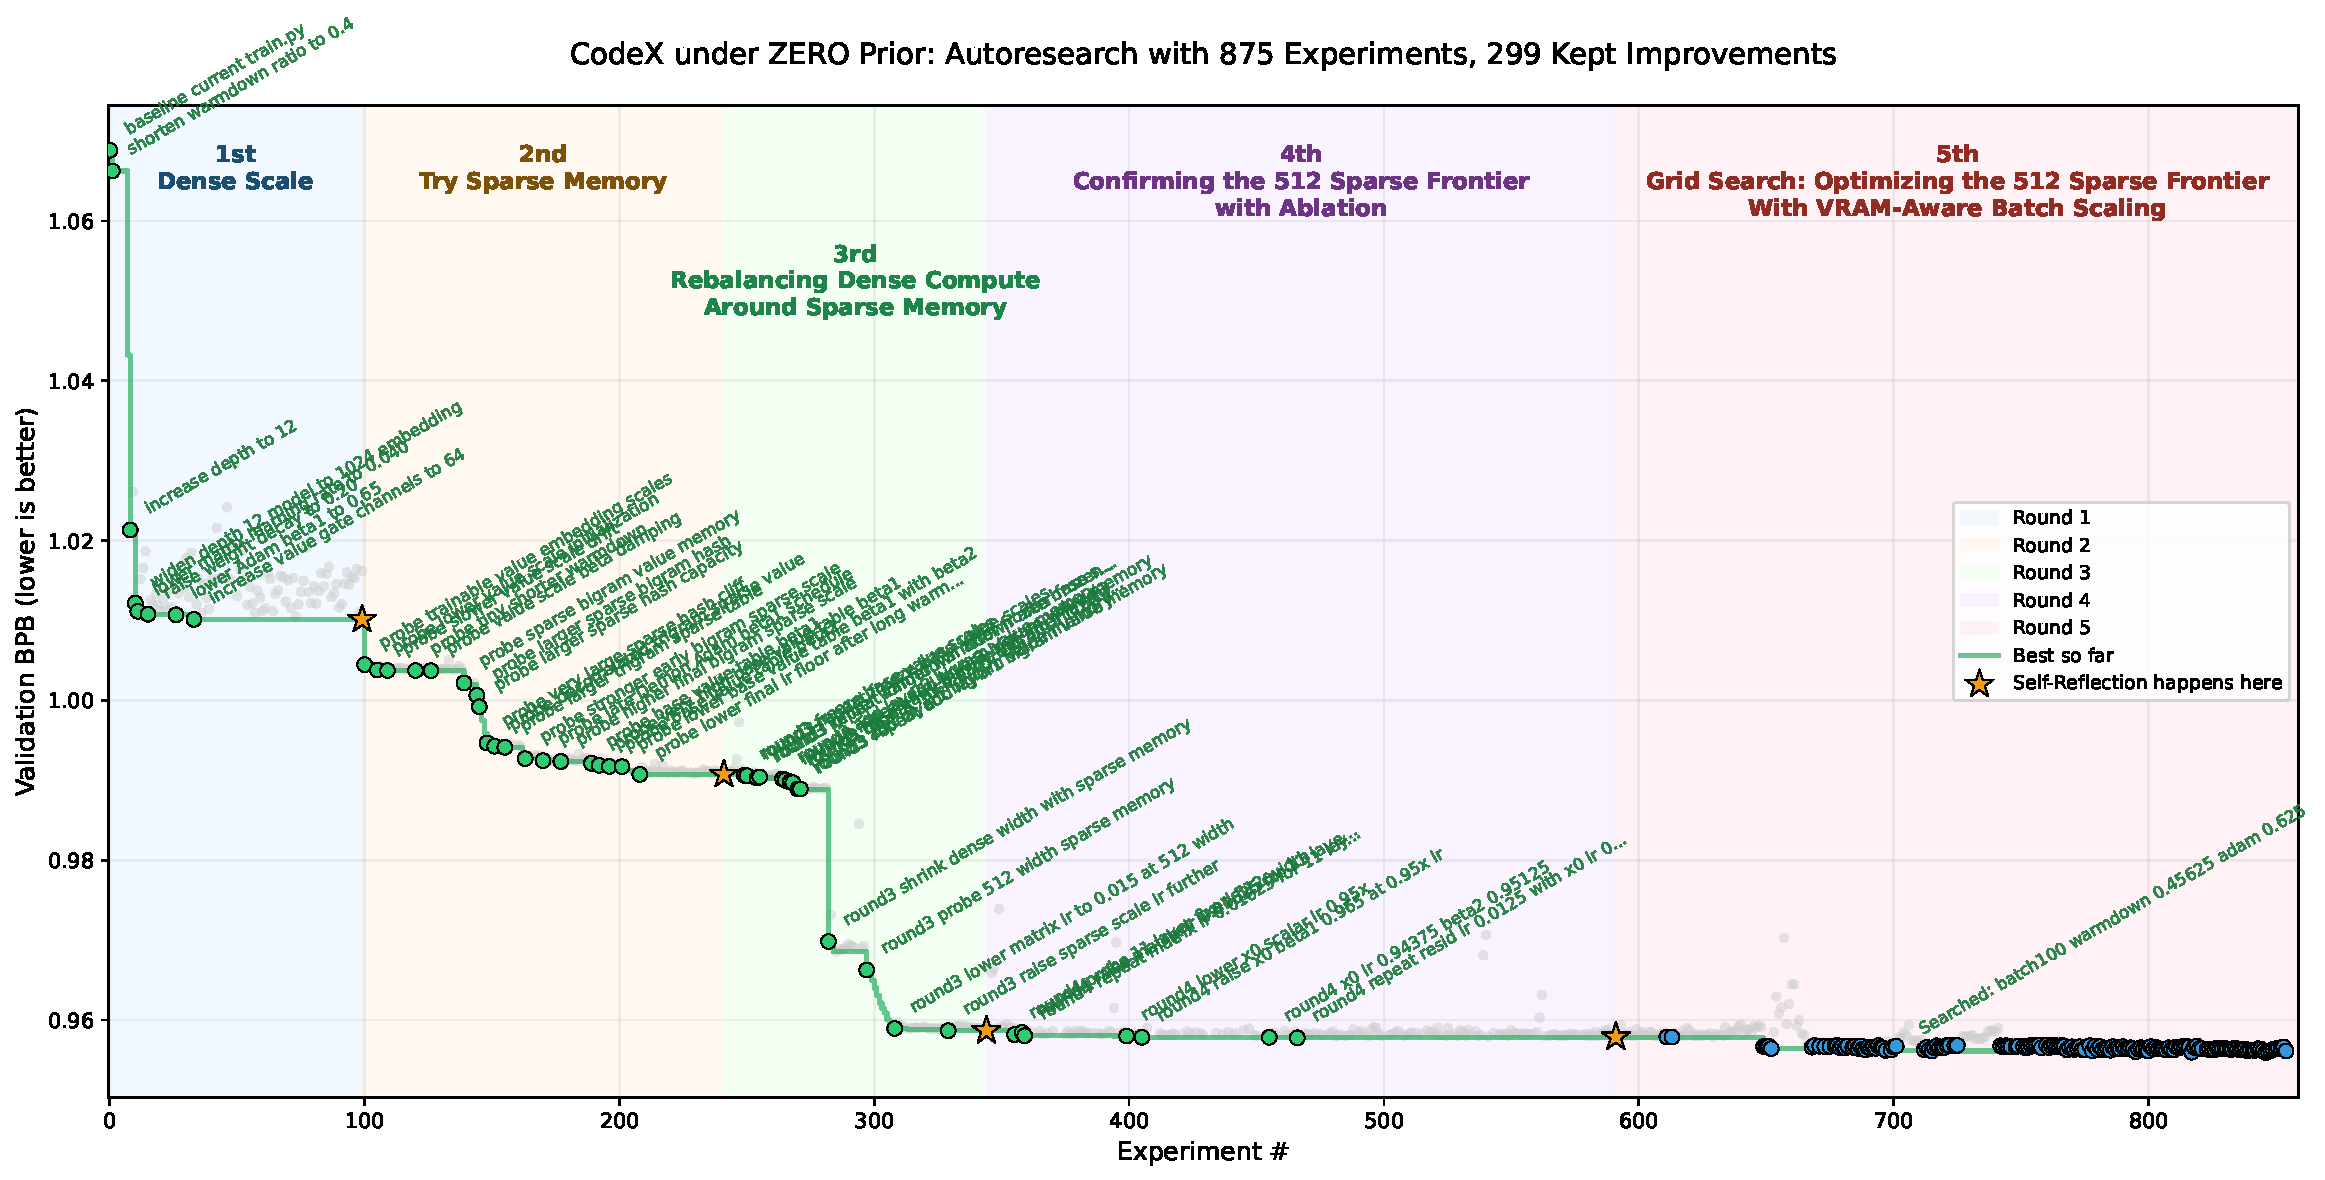
\includegraphics[width=\linewidth]{figure/pure_LLM_autoresearch_progress.pdf}
    \caption{\textbf{Pure LLM research loop on \texttt{autoresearch}.} Validation \texttt{val\_bpb} (lower is better) across $875$ no-BO, no-acquisition experiments. Gray points are individual trials and the green step curve is the best value found so far; yellow stars mark self-reflection checkpoints where the agent summarises the ledger and enters a new research regime. The coloured bands show the loop's staged progress: dense scaling, sparse-memory invention, dense-compute rebalancing around sparse memory, ablation-based confirmation of the $512$-sparse frontier, and final VRAM-aware batch/schedule search. The curve demonstrates that a pure LLM loop can do real sequential research, but also its ceiling: after the large regime shifts it plateaus near $\texttt{val\_bpb}\approx0.956$, above the LDM result of $0.93421$ in Figure~\ref{fig:autoresearch}.}
    \label{fig:abl-pure-llm}
\end{figure}

Figure~\ref{fig:abl-pure-llm} shows that the pure LLM loop is not inert. It discovers several coherent research phases: first dense scaling, then sparse memory, then a rebalance of dense compute around the sparse memory idea, followed by confirmation and grid search around the $512$-sparse frontier. The best-so-far curve falls from the initial $\texttt{val\_bpb}\approx1.069$ to $\approx1.01$ after the first phase, to $\approx0.991$ after the second reflection, and to $\approx0.959$ after the sparse-frontier breakthrough. In other words, a modern code agent with a task-specific prompt and access to its own run log can already produce human-readable, scientifically reasonable progress: it can form hypotheses, translate them into code edits, test them, preserve improvements, and revise its research state.

The archived loop logs show what this ``research work'' consisted of. The agent did not merely enumerate nearby hyperparameters. After each phase it wrote a reflection report: it compressed the ledger into mechanistic claims, labelled memories by regime and mechanism, retrieved positive and negative examples, and used the labelled memories to choose the next experiment family. Table~\ref{tab:pure-llm-trace} summarises the resulting trajectory. The important point is the \emph{statefulness}: the loop changes what it believes the problem is. It begins with ordinary dense scaling, decides that dense capacity has saturated under the five-minute budget, invents sparse associative value memory as a cheaper capacity axis, then shrinks the dense core so that the sparse-memory model can train in time, and finally switches to repeat-first, VRAM-aware frontier tuning once improvements fall into the noise band.

\begin{table}[t]
    \centering
    \footnotesize
    \begin{tabular}{p{0.11\linewidth}p{0.20\linewidth}p{0.37\linewidth}p{0.14\linewidth}}
        \toprule
        Phase & Working hypothesis & Evidence generated by the loop & Best \texttt{val\_bpb} \\
        \midrule
        Dense scaling & Capacity is the early bottleneck, but only while the model can still be trained inside the fixed budget.
        & Depth $10$ and $12$ give large drops; widening the depth-$12$ model helps; depth $14$ worsens near the memory ceiling. The reflection turns this into the rule: dense capacity helps until the update budget becomes the bottleneck.
        & $1.010136$ \\
        Sparse value memory & Dense capacity is saturated, but cheap associative capacity may still help if routed through a bounded value path.
        & Trainable value scales, sparse hashed bigram memory, larger hash tables, decorrelated trigram memory, and phase-specific damping improve the frontier; broader routing and optimizer rewires are recorded as negative memories.
        & $0.990738$ \\
        Dense-compute rebalance & Sparse memory works best when the dense core is smaller and no longer steals the fixed training budget.
        & Causal ablations show trigram memory, early bigram memory, and trainable sparse scales matter. Shrinking dense width to $640$ and then $512$ creates the large breakthrough, after which matrix LR, final LR floor, and sparse-scale LR are retuned.
        & $0.958666$ \\
        Frontier confirmation & The $512$ sparse-memory regime is a narrow compute/update-budget island, and remaining gains require repeats.
        & Widths below and above $512$ lose; removing early ngram memory increases throughput but hurts validation, showing the memory path is causal. Restored-anchor repeats estimate a noise floor of roughly $3$--$5\times10^{-4}$ BPB.
        & $0.957766$ \\
        VRAM-aware batch tuning & Spare VRAM should buy batch/throughput and coupled schedule tuning, not a return to dense scaling.
        & The context retrieves the dense-shrink successes and negative memories against larger dense models, then grid-searches batch size, warmdown, final LR, Adam damping, and weight decay while logging steps, tokens, MFU, and loss slopes.
        & $0.955923$ \\
        \bottomrule
    \end{tabular}
    \caption{\textbf{Mechanistic trace of the pure LLM research loop.} Each row is a phase extracted from the loop logs. The LLM acts like a lightweight experimental scientist: it writes a hypothesis, tests code-level interventions, records both successes and failures, updates a regime label, and carries those memories into the next phase.}
    \label{tab:pure-llm-trace}
\end{table}

This trace is the strongest evidence that the baseline is a genuine research loop. It performs causal ablations (for example, removing trigram memory, early bigram memory, or sparse scales), estimates the noise floor by repeating restored anchors, and eventually augments the ledger with trajectory diagnostics such as steps, tokens, MFU, train/eval gap, and loss slopes. It also learns what not to do: the contexts explicitly retrieve failed routing rewires, failed dense-width probes, crashes, and repeated optimizer mismatches as negative memories. In short, the loop accumulates procedural knowledge, not just a list of winning commits.

The limitation is equally visible. After the third breakthrough, the remaining $\approx500$ experiments are mostly local confirmation and grid search around the same frontier. The loop continues to keep small improvements, but the envelope is nearly flat, ending around $\texttt{val\_bpb}\approx0.956$. This is better than the no-discover Karpathy baseline in Figure~\ref{fig:autoresearch}, which stalls at $0.9767$, but it is still far from the LDM curve, which reaches $0.93421$ under the same H100 five-minute-run setting. The pure LLM loop can reason about its own transcript and name plausible new regimes, but between those reflections it has no calibrated estimate of where improvement is likely, where uncertainty remains high, or when a plateau is evidence that the current boundary is exhausted.

This is the ablation's main conclusion. The bottleneck is not proposal expressivity: the LLM can write useful training code, exploit prior knowledge about how the architecture can be modified, and remember enough of the transcript to pursue multi-stage ideas. The bottleneck is value. Without $\mu_t$, $\sigma_t$, and the acquisition $\acq_t$, \textbf{the run log remains a narrative memory rather than a searchable value landscape}. LDM supplies exactly that missing object: the surrogate turns the same history into a posterior over the program space, and the acquisition turns that posterior into a decision value for both local refinement and boundary-moving discover steps. The pure LLM loop therefore validates the reservoir side of the framework and shows how far current agent systems can already go, while also showing why the BO-value side is necessary for the performance gains in the main experiment.

\subsection{Test-time Search for LDM}
\label{app:abl-ldm}

This ablation asks whether LDM exhibits the same test-time scaling behaviour that motivates inference-time search in language-model reasoning \citep{snell2025scaling}, but in the harder setting where the value is an expensive scientific objective approximated by a surrogate. We keep the outer evaluation budget fixed and vary only the cheap inner-loop budget of LDM-TTS. Concretely, the inner budget has four knobs: (i) how many candidate programmes the LLM proposes at each outer iteration, (ii) how many hypothesis or refinement branches the BO inner loop expands for each candidate before scoring, (iii) how many of those scored candidates the acquisition retains for the next round, and (iv) which acquisition function scores them. The detailed \texttt{autoresearch} test-time-search sweep, with its N4H4/N8H8 budgets and EI vs. posterior-mean comparison, already appears in Section~\ref{sec:ablation-main}; here we keep only the molecule and CDRH3 single-step budget sweeps.

The theory in \S\ref{sec:theory-main} predicts exactly this dependence: increasing the near-acquisition mass available to the tilted sampler reduces the LDM sampling shortfall term, but only if the added candidates are also evaluated by a calibrated value model rather than by language plausibility alone.

\subsubsection{Small-molecule drug discovery}
\label{app:abl-molecule}

The molecular ablation repeats the same question in a chemically open-ended space. Here the expensive evaluation is a two-objective KRAS G12D score, and performance is the dominated Pareto hypervolume under the Vina/activity objectives of \S\ref{sec:cs-molecule-results}. We use the Direct-Softmax LDM pipeline with a Qwen3.5-9B proposer and vary two inner-loop budgets. A label \texttt{proposer}\{K\}\_\texttt{bo}\{M\} means that the LLM proposes a pool of $K$ candidate SMILES strings and the BO/EHVI inner loop is allowed to score up to $M$ candidates and retain the best-scoring ones before the next expensive molecular evaluation is chosen. Thus $K$ controls the breadth of the LLM reservoir draw, while $M$ controls how much of that breadth is exposed to the calibrated multi-objective value.

\begin{figure}[htbp]
    \centering
    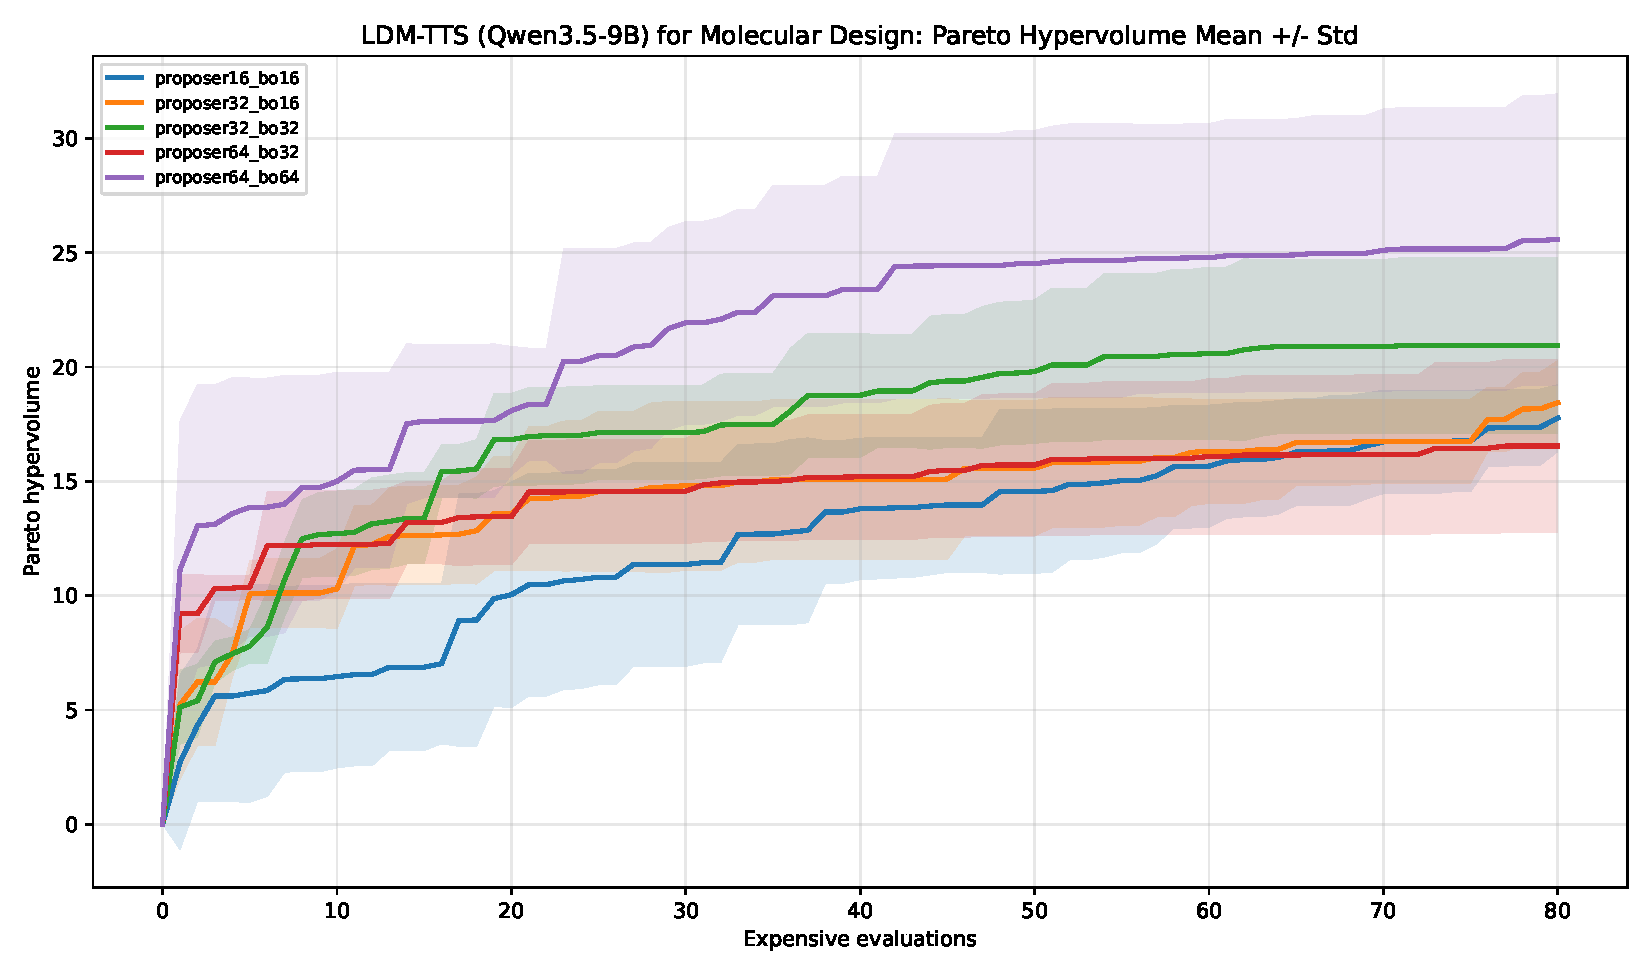
\includegraphics[width=0.8\linewidth]{figure/qwen3_9B_pareto_hypervolume_mean_std.pdf}
    \caption{\textbf{Test-time search scaling for molecular design.} Pareto hypervolume (higher is better) over expensive molecular evaluations for Qwen3.5-9B Direct-Softmax LDM-TTS. Curves show the mean over independent runs, with shaded bands denoting one standard deviation; legend entries report the LLM proposal budget and BO/EHVI acquisition-scoring budget. Balanced scaling of both budgets improves hypervolume most: \texttt{proposer64\_bo64} reaches the strongest final Pareto front, while increasing proposals without matching acquisition bandwidth gives smaller or unstable gains.}
    \label{fig:abl-molecule-tts}
\end{figure}

\begin{figure}[htbp]
    \centering
    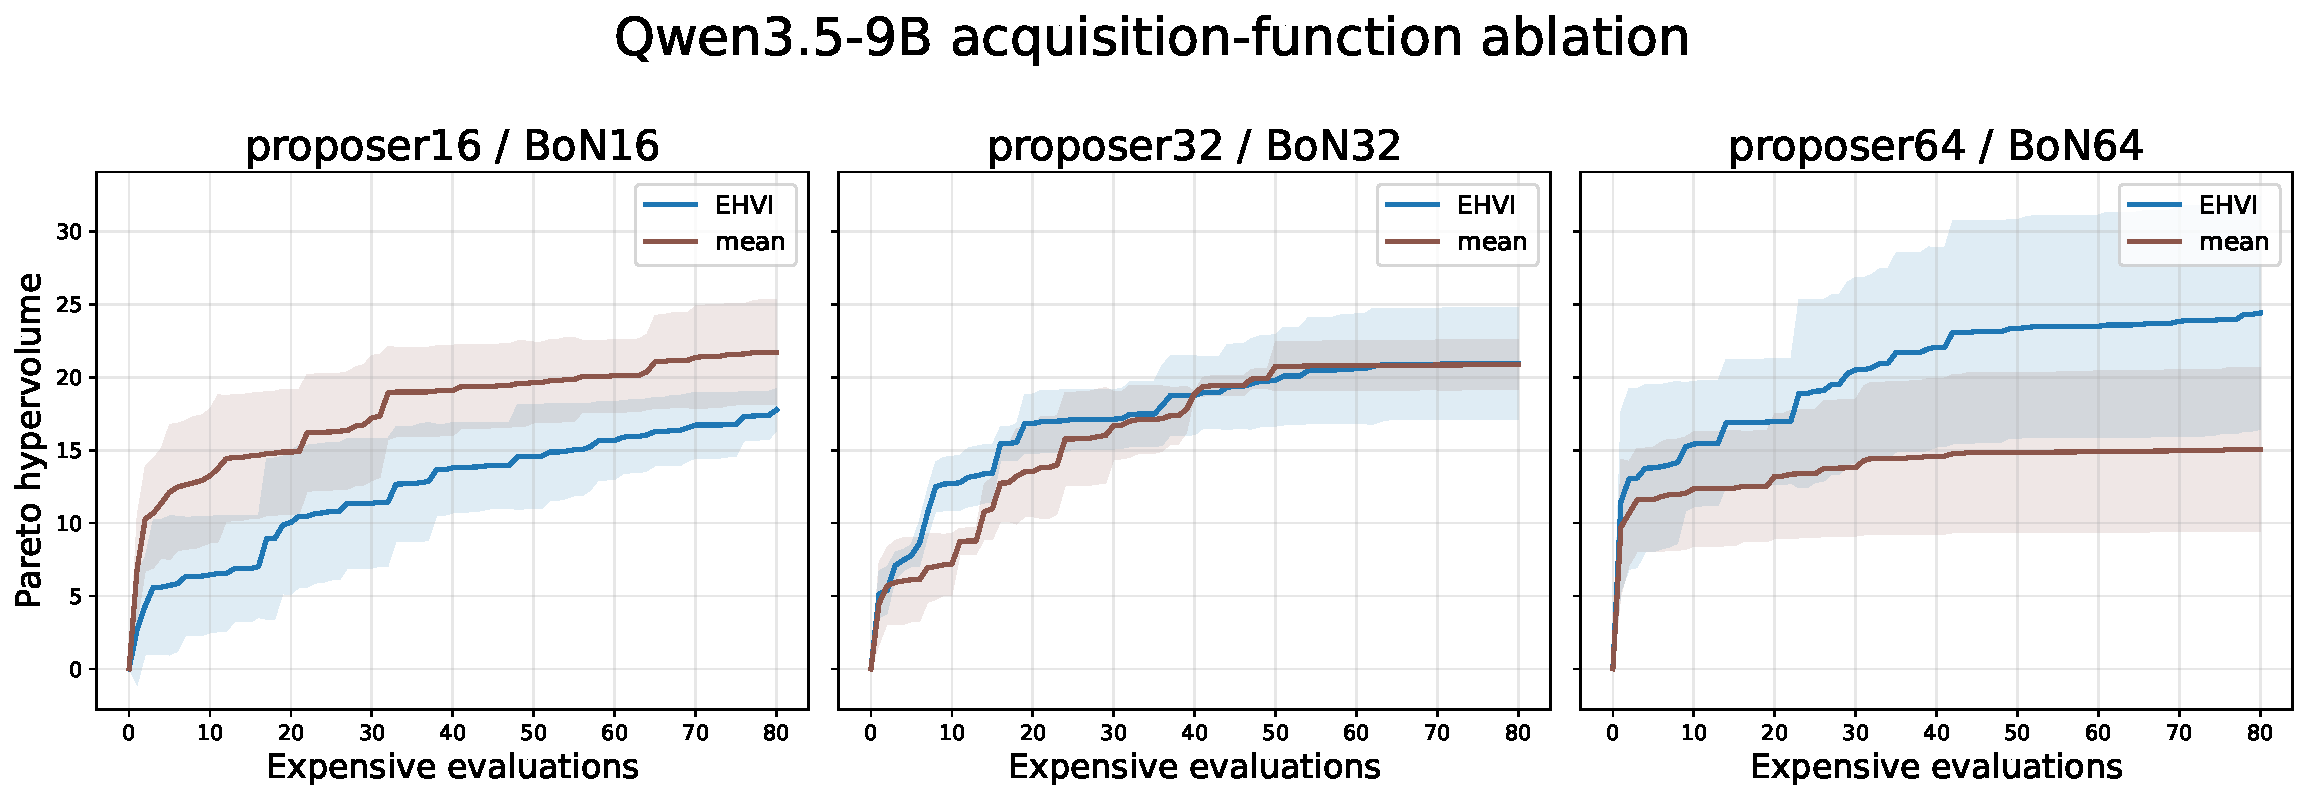
\includegraphics[width=\linewidth]{figure/qwen3_9B_acquisition_ablation_hypervolume.pdf}
    \caption{Abaltion on acquisition function over different search budgets for molecular design.}
    \label{fig:placeholder2}
\end{figure}

Figure~\ref{fig:abl-molecule-tts} shows that test-time compute also scales in the molecular setting, but only when both inner budgets grow together. Increasing the LLM proposal budget from $16$ to $32$ improves the curve, and increasing the BO/EHVI scoring budget from $16$ to $32$ improves it further: \texttt{proposer32\_bo32} dominates the smaller-budget settings through most of the run. \texttt{proposer64\_bo64} makes the largest early jump and keeps the highest final hypervolume; the asymmetric \texttt{proposer64\_bo32} does worse, which shows that broad SMILES generation is useful only when the EHVI side has enough bandwidth to filter the resulting candidates.

Figure~\ref{fig:placeholder2} adds the acquisition-function dimension. At small budgets, mean- or UCB-style acquisitions (a $0.5/0.5$ weighted scalarisation of the Vina and activity objectives) outperform the strict EHVI; as $n$ grows, EHVI overtakes them and continues to improve, while mean-style acquisitions degrade or stagnate. The mechanism is bandwidth: EHVI is built on the strict Pareto frontier and therefore needs a large screening budget to be effective, because multi-objective improvements correspond to sparse non-dominated points. Mean-style acquisitions collapse the two objectives into one scalar, so at small budgets the per-step randomness from a thin screening budget partially substitutes for the missing Pareto signal, smoothing out the optimisation and keeping the curve flat; once the budget grows, EHVI's strict-screening advantage takes over.

\subsubsection{Antibody CDRH3 design}
\label{app:abl-antibody}

% \begin{figure}[t]
%     \centering
%     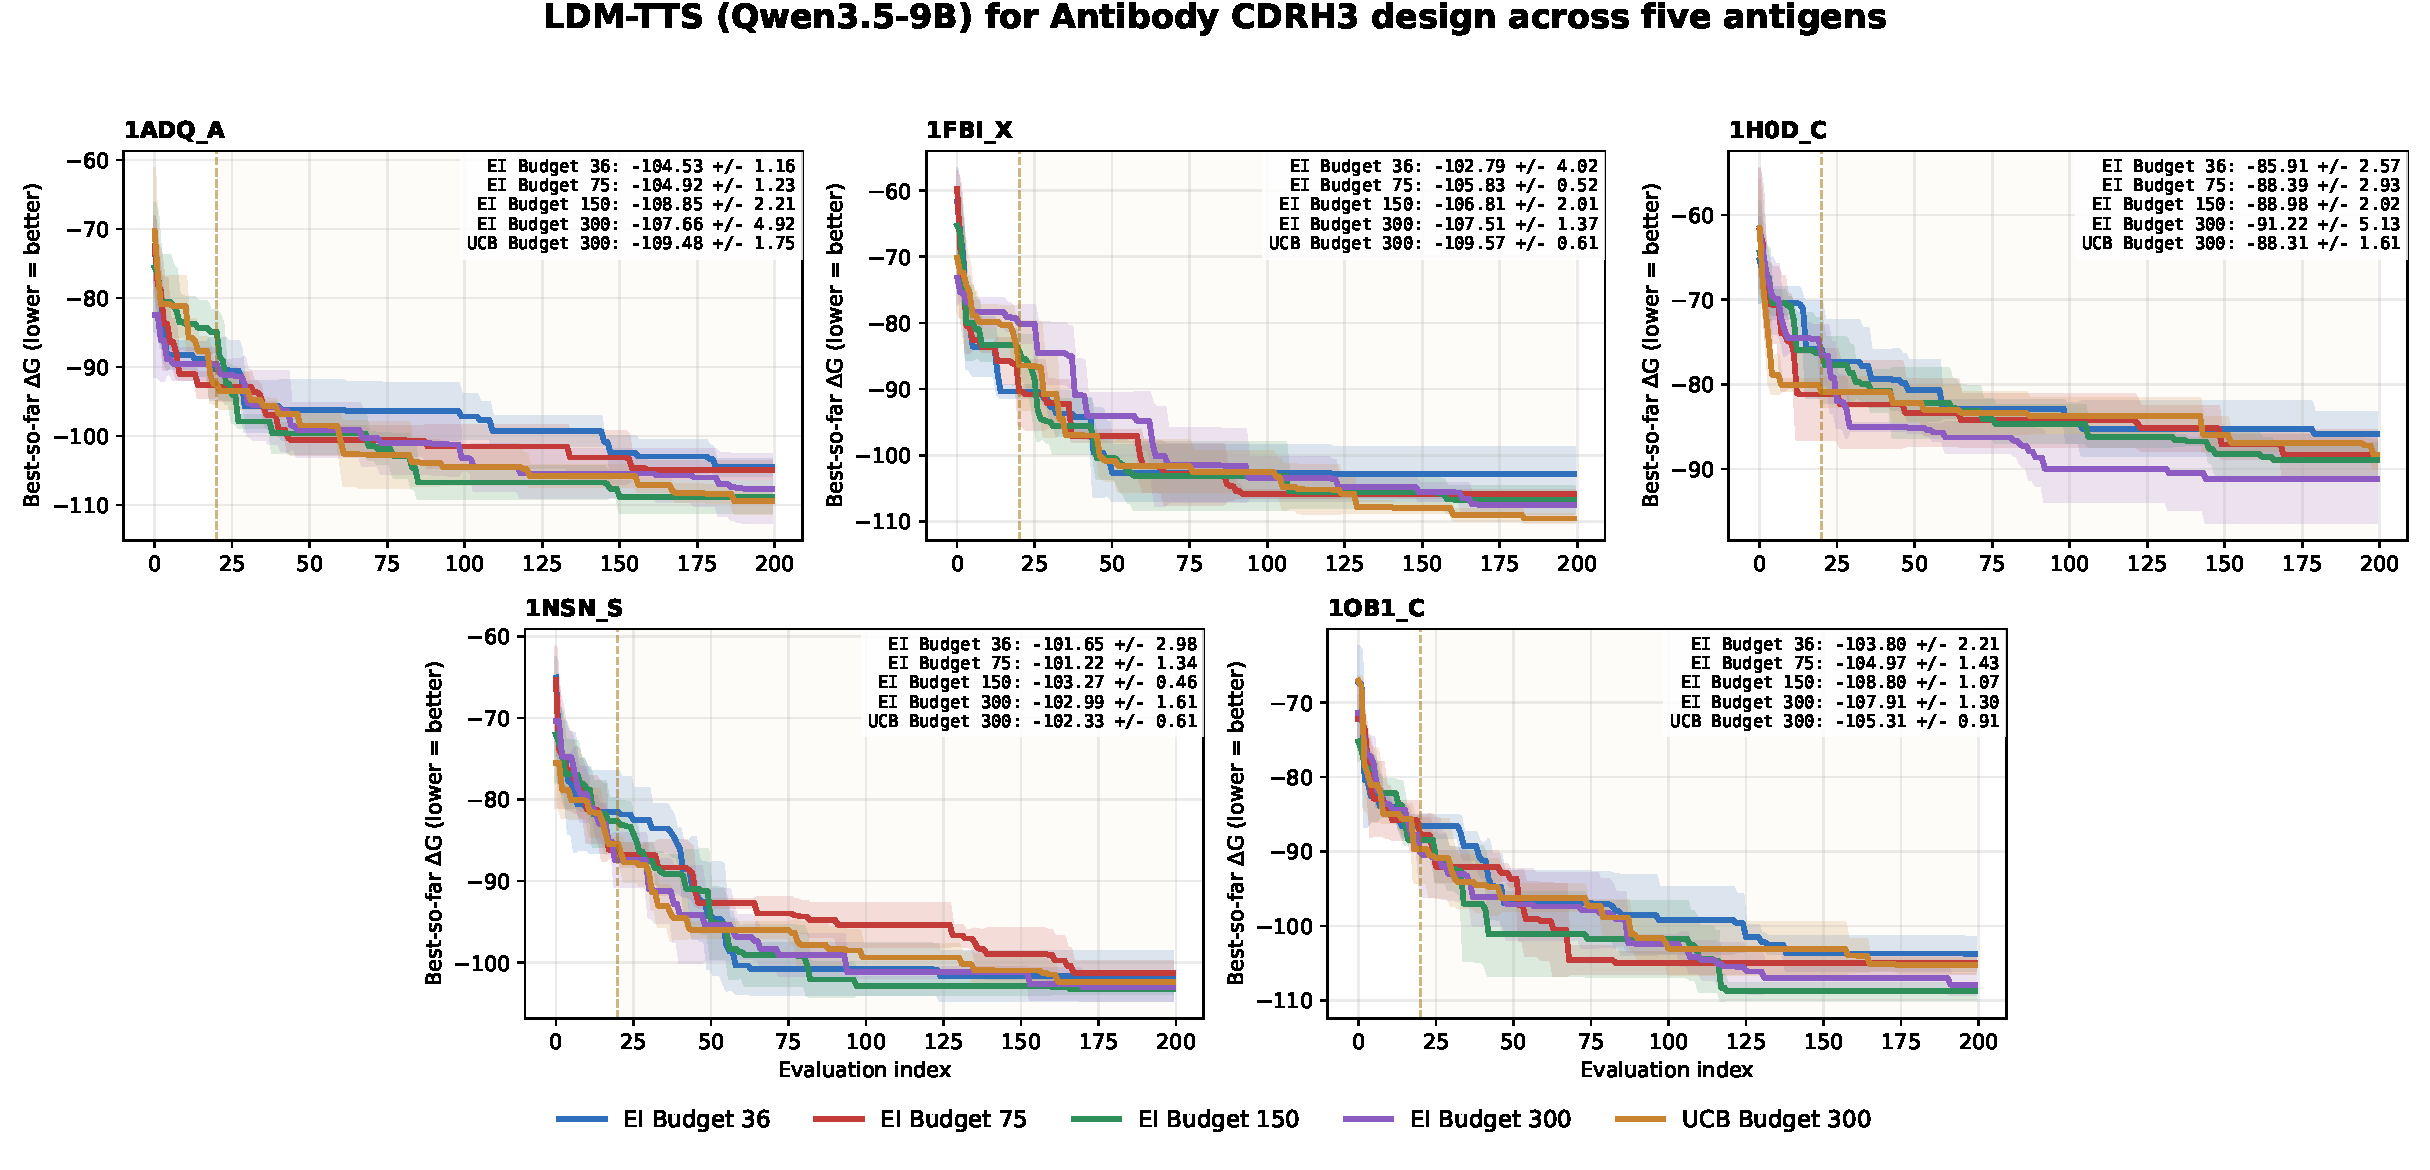
\includegraphics[width=\linewidth]{figure/LDM-TTS-Antigens.pdf}
%     \caption{\textbf{Test-time search scaling for antibody CDRH3 design.} Best-so-far \textsc{Absolut!} binding energy (lower is better) for Qwen3.5-9B LDM-TTS across five antigens. The expensive evaluation budget is fixed at $200$ oracle calls per target. Legend entries vary the LLM proposer budget, i.e., the number of candidate CDRH3 sequences or sequence-neighbourhood samples generated before each oracle query; the BO search budget is not independently tuned and is set to the maximum available number of remaining proposals after filtering. Shaded bands denote one standard deviation across seeds, and panel annotations report the final mean $\pm$ standard deviation. Moderate-to-large proposer budgets improve over the smallest budget on all targets, with the strongest final setting usually occurring at budget $150$ or $300$, showing that additional open-source LLM test-time compute can be converted into better CDRH3 designs when filtered by the BO acquisition.}
%     \label{fig:abl-antigen-tts}
% \end{figure}

% \begin{figure}
%     \centering
%     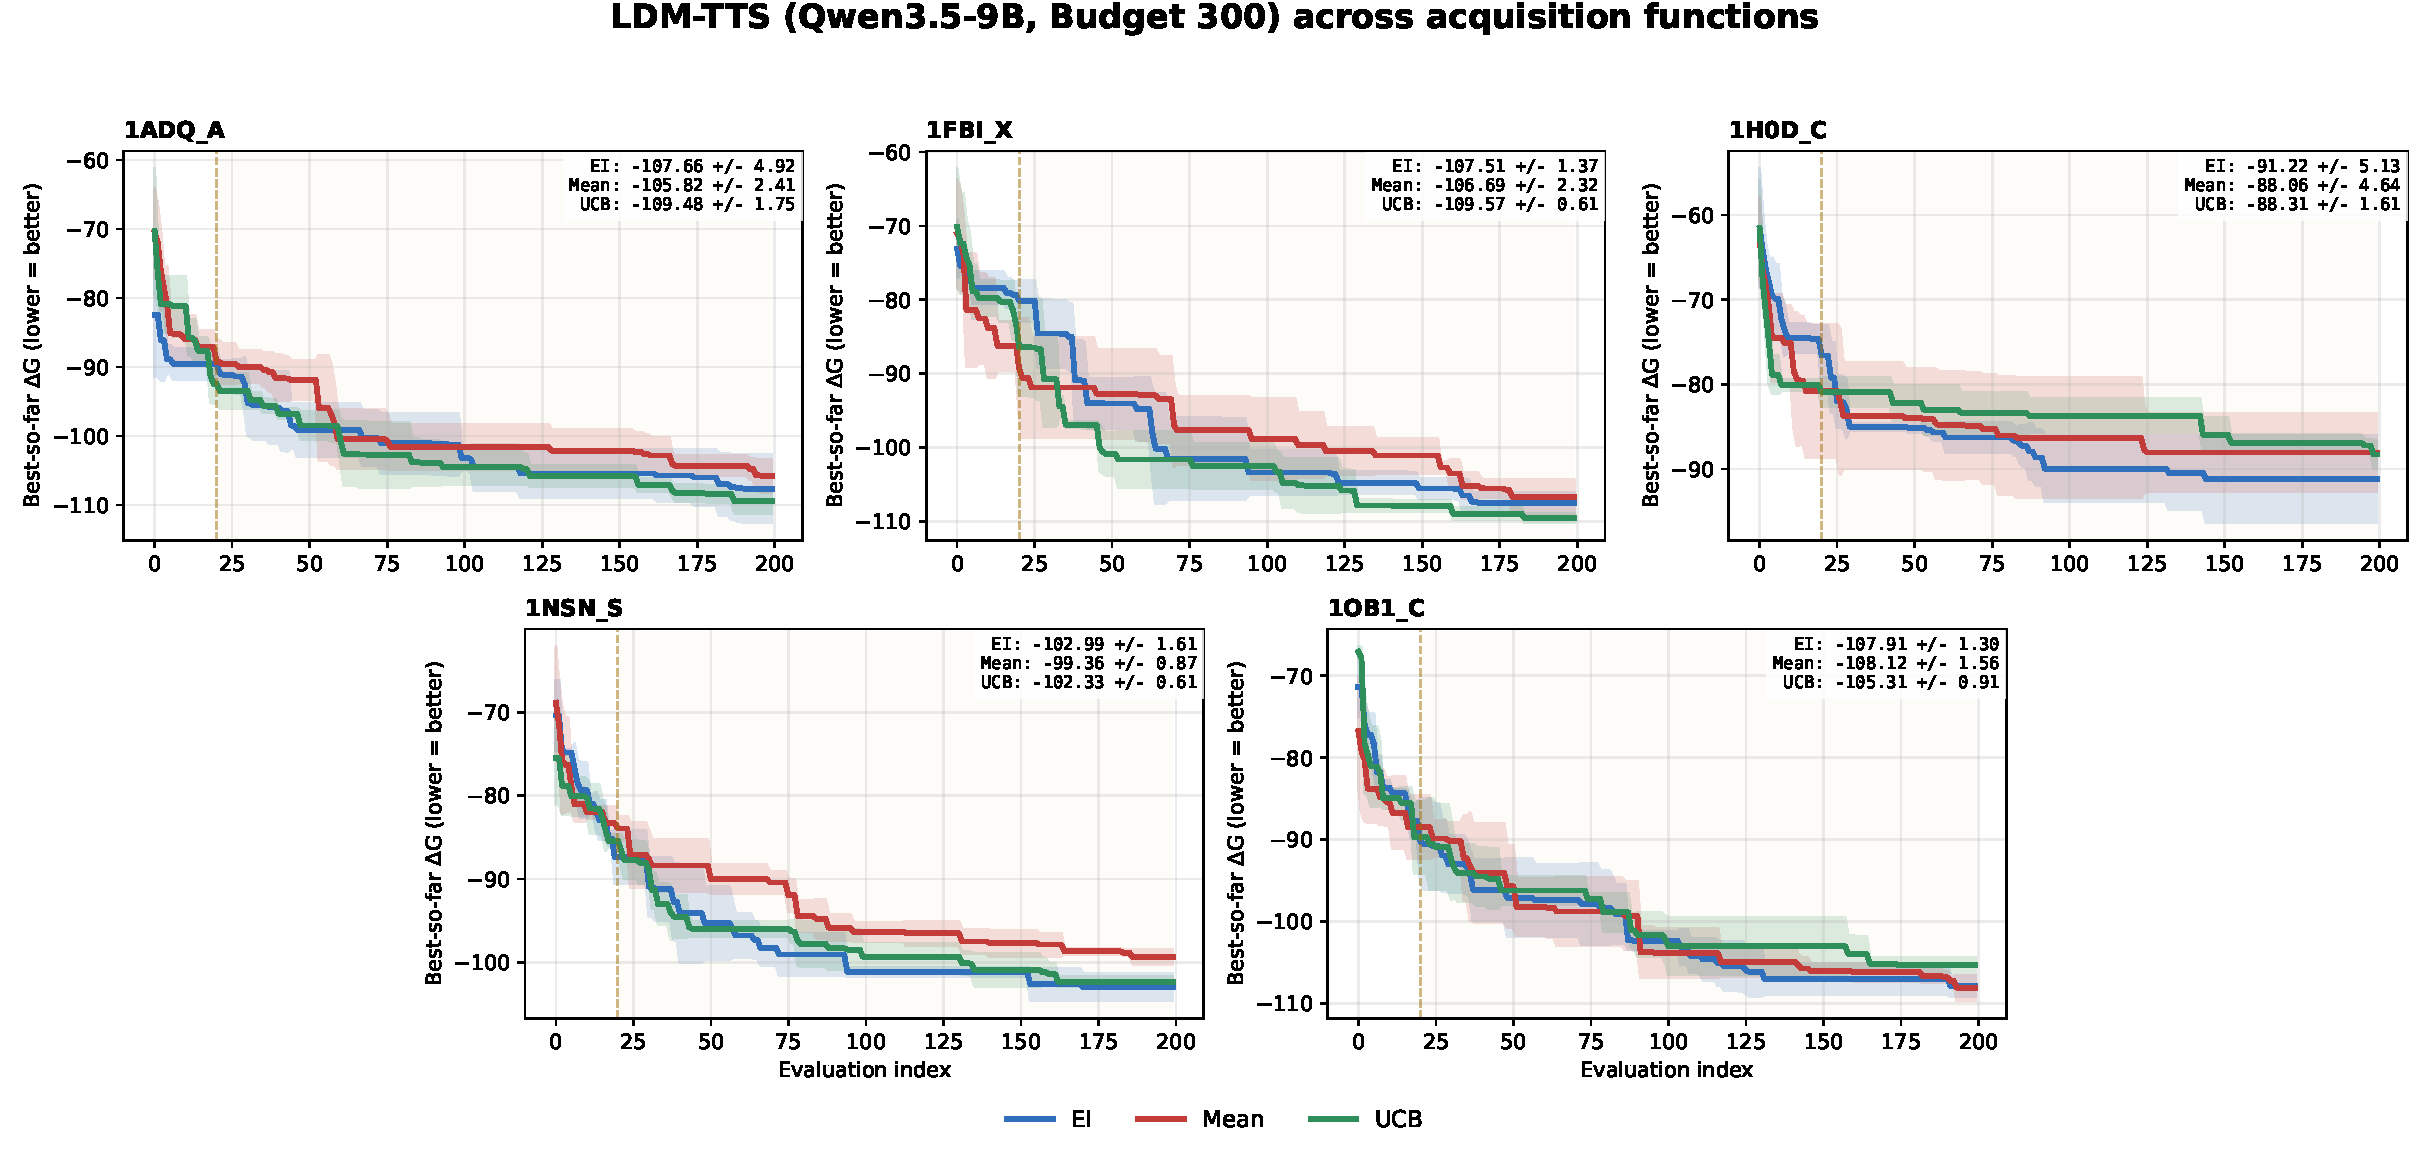
\includegraphics[width=\linewidth]{figure/budget300_acquisition_comparison_5subplots.pdf}
%     \caption{LDM-TTS across acquisition functions}
%     \label{fig:placeholder3}
% \end{figure}

% \begin{figure}
%     \centering
%     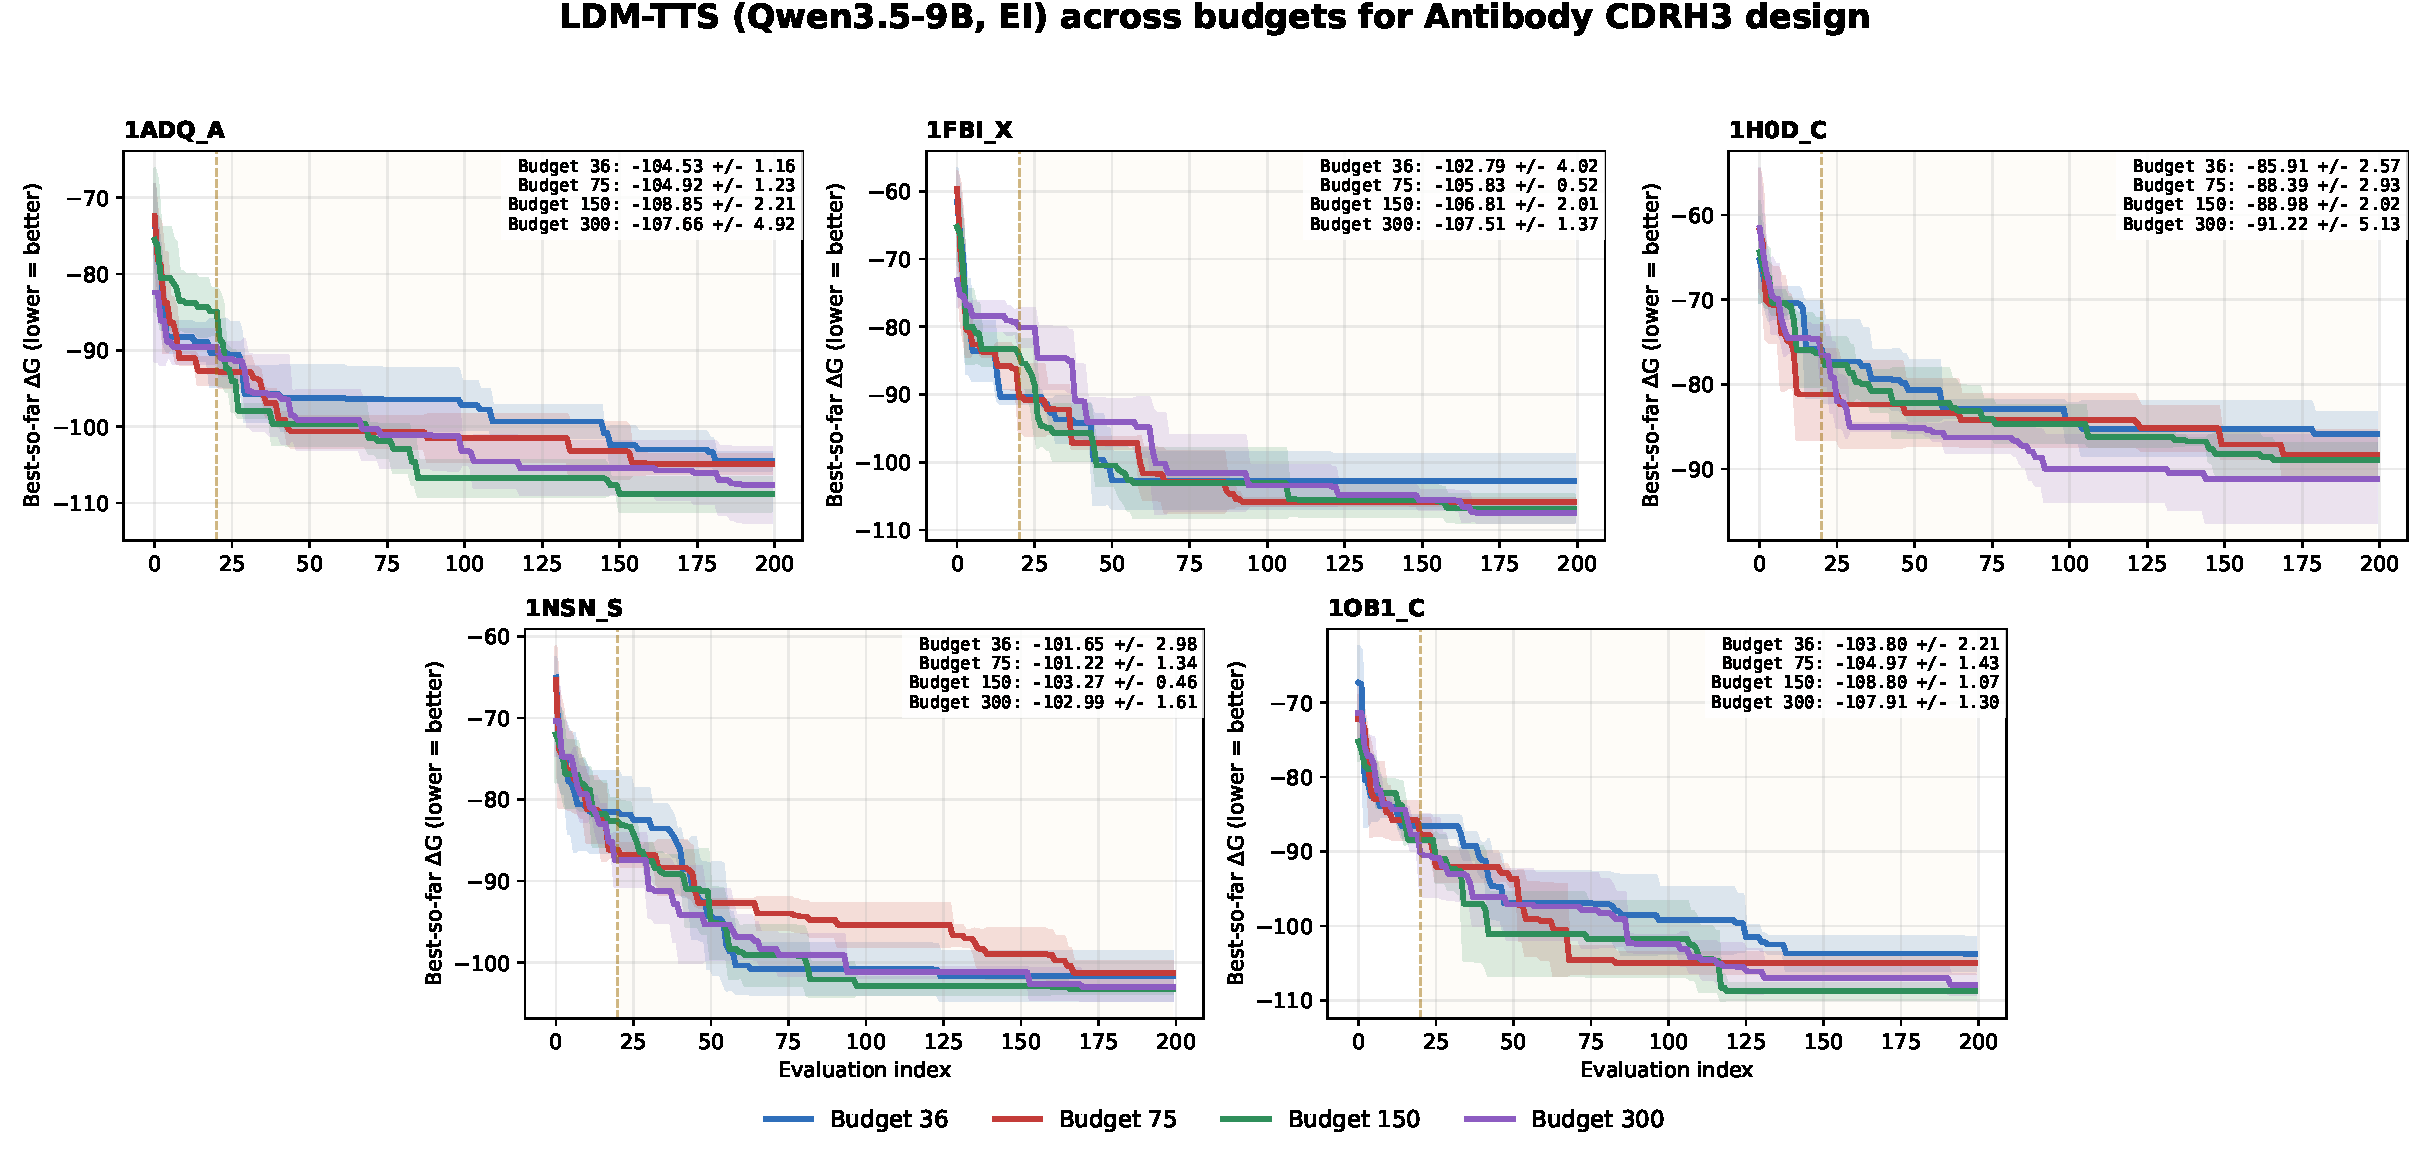
\includegraphics[width=\linewidth]{figure/ei_budget_comparison_5subplots.pdf}
%     \caption{LDM-TTS across budget for Antibody CDRH3 design}
%     \label{fig:placeholder4}
% \end{figure}

\begin{figure}
    \centering
    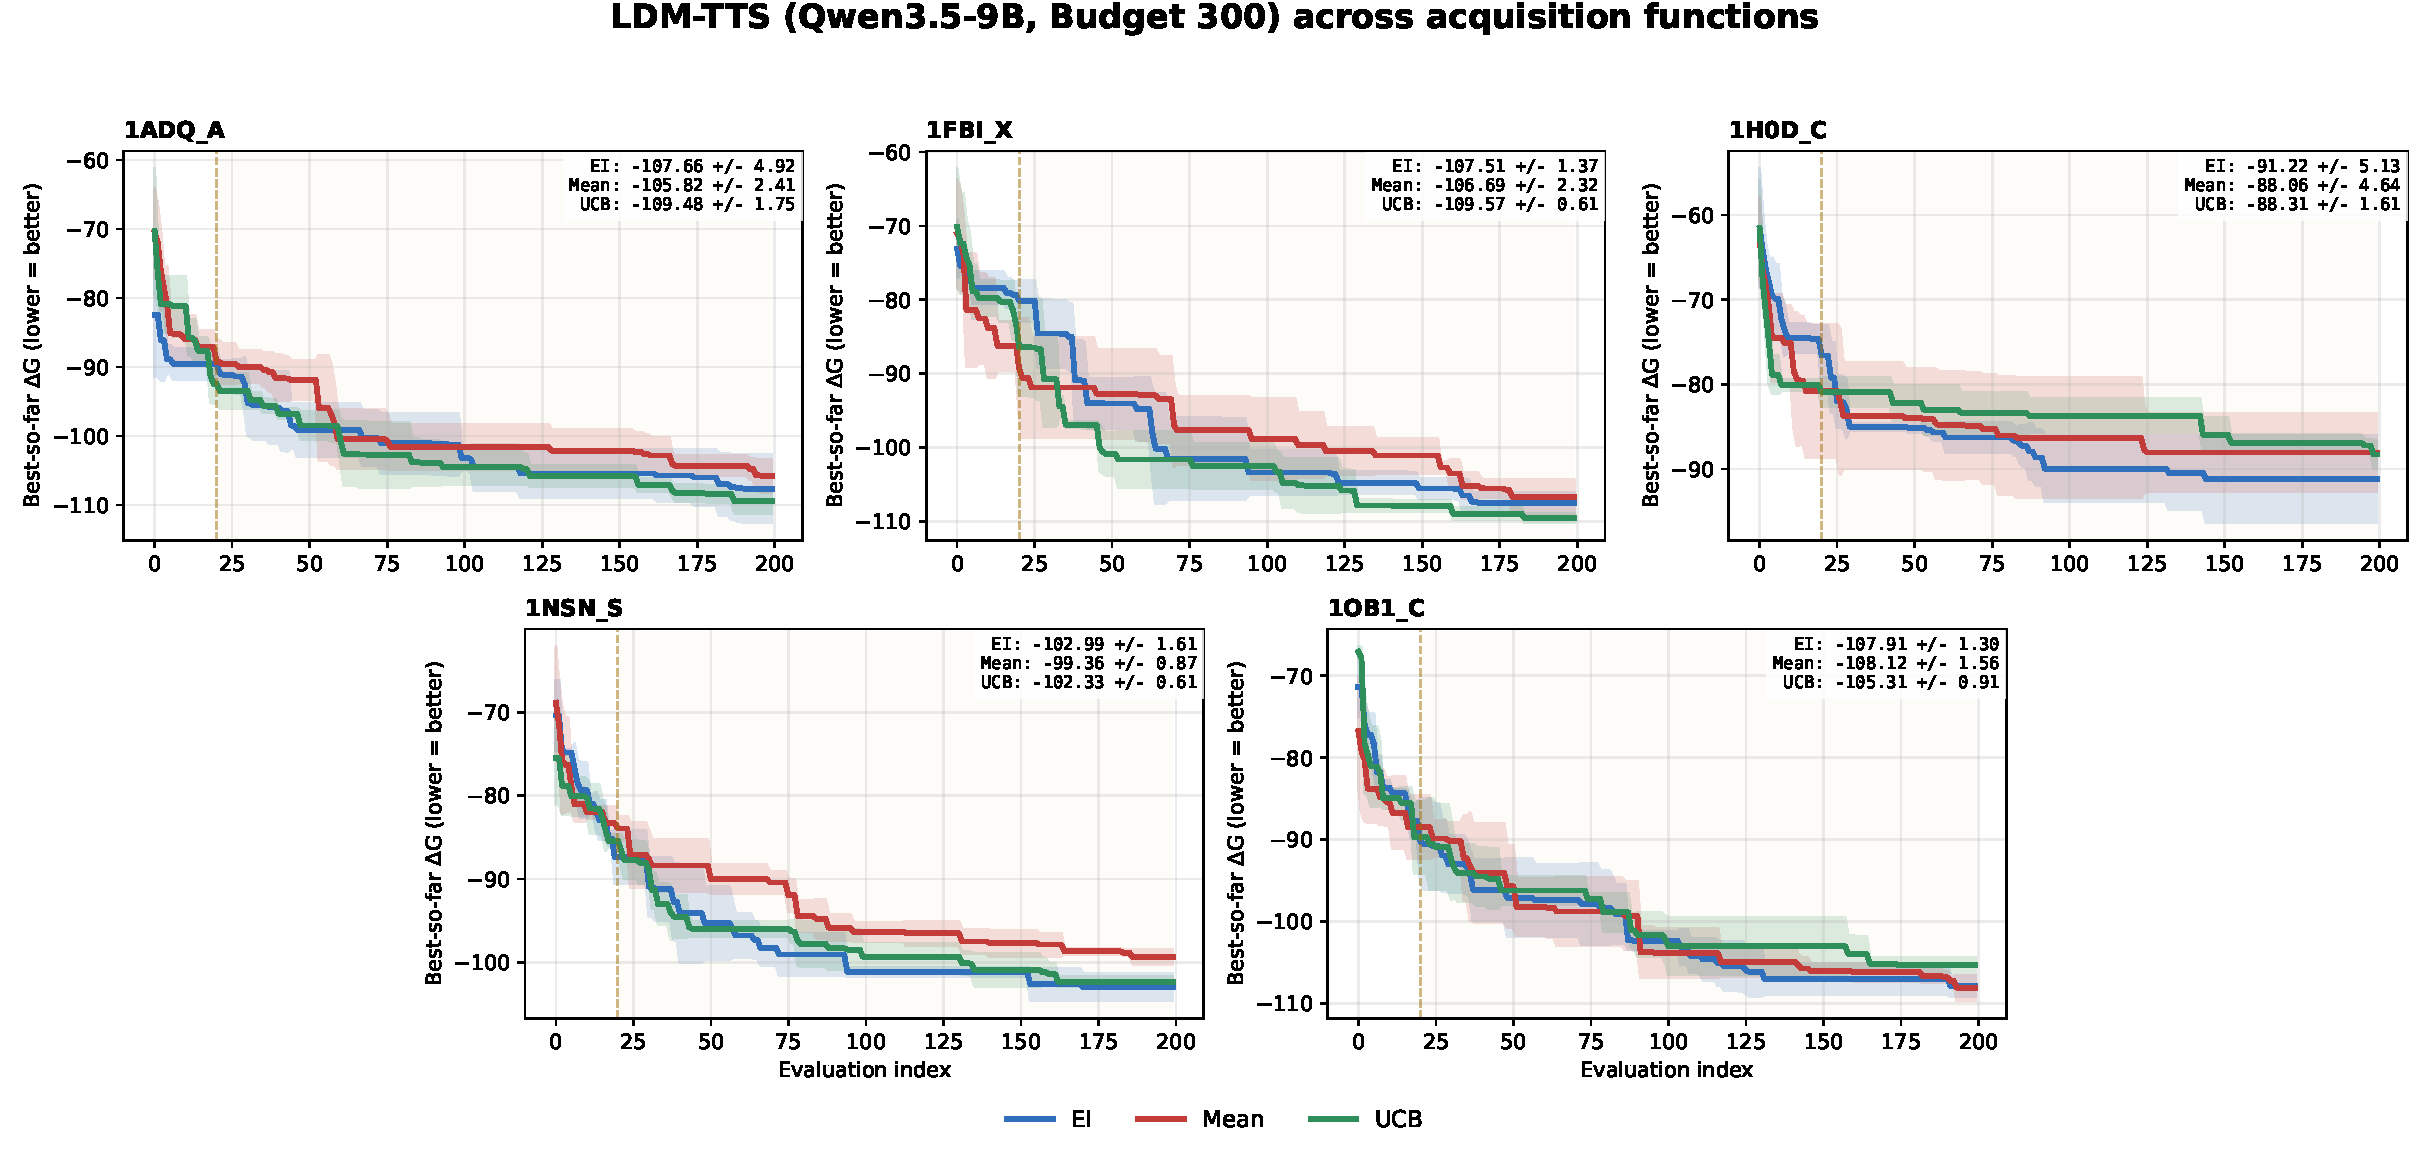
\includegraphics[width=\linewidth]{figure/budget300_acquisition_comparison_5subplots.pdf}
    \caption{Comparison of different acquisition functions for LDM-TTS with a fixed proposer budget of 300 on Antibody CDRH3 design.}
    \label{fig:abl-antigen-acquisition}
\end{figure}

\begin{figure}
    \centering
    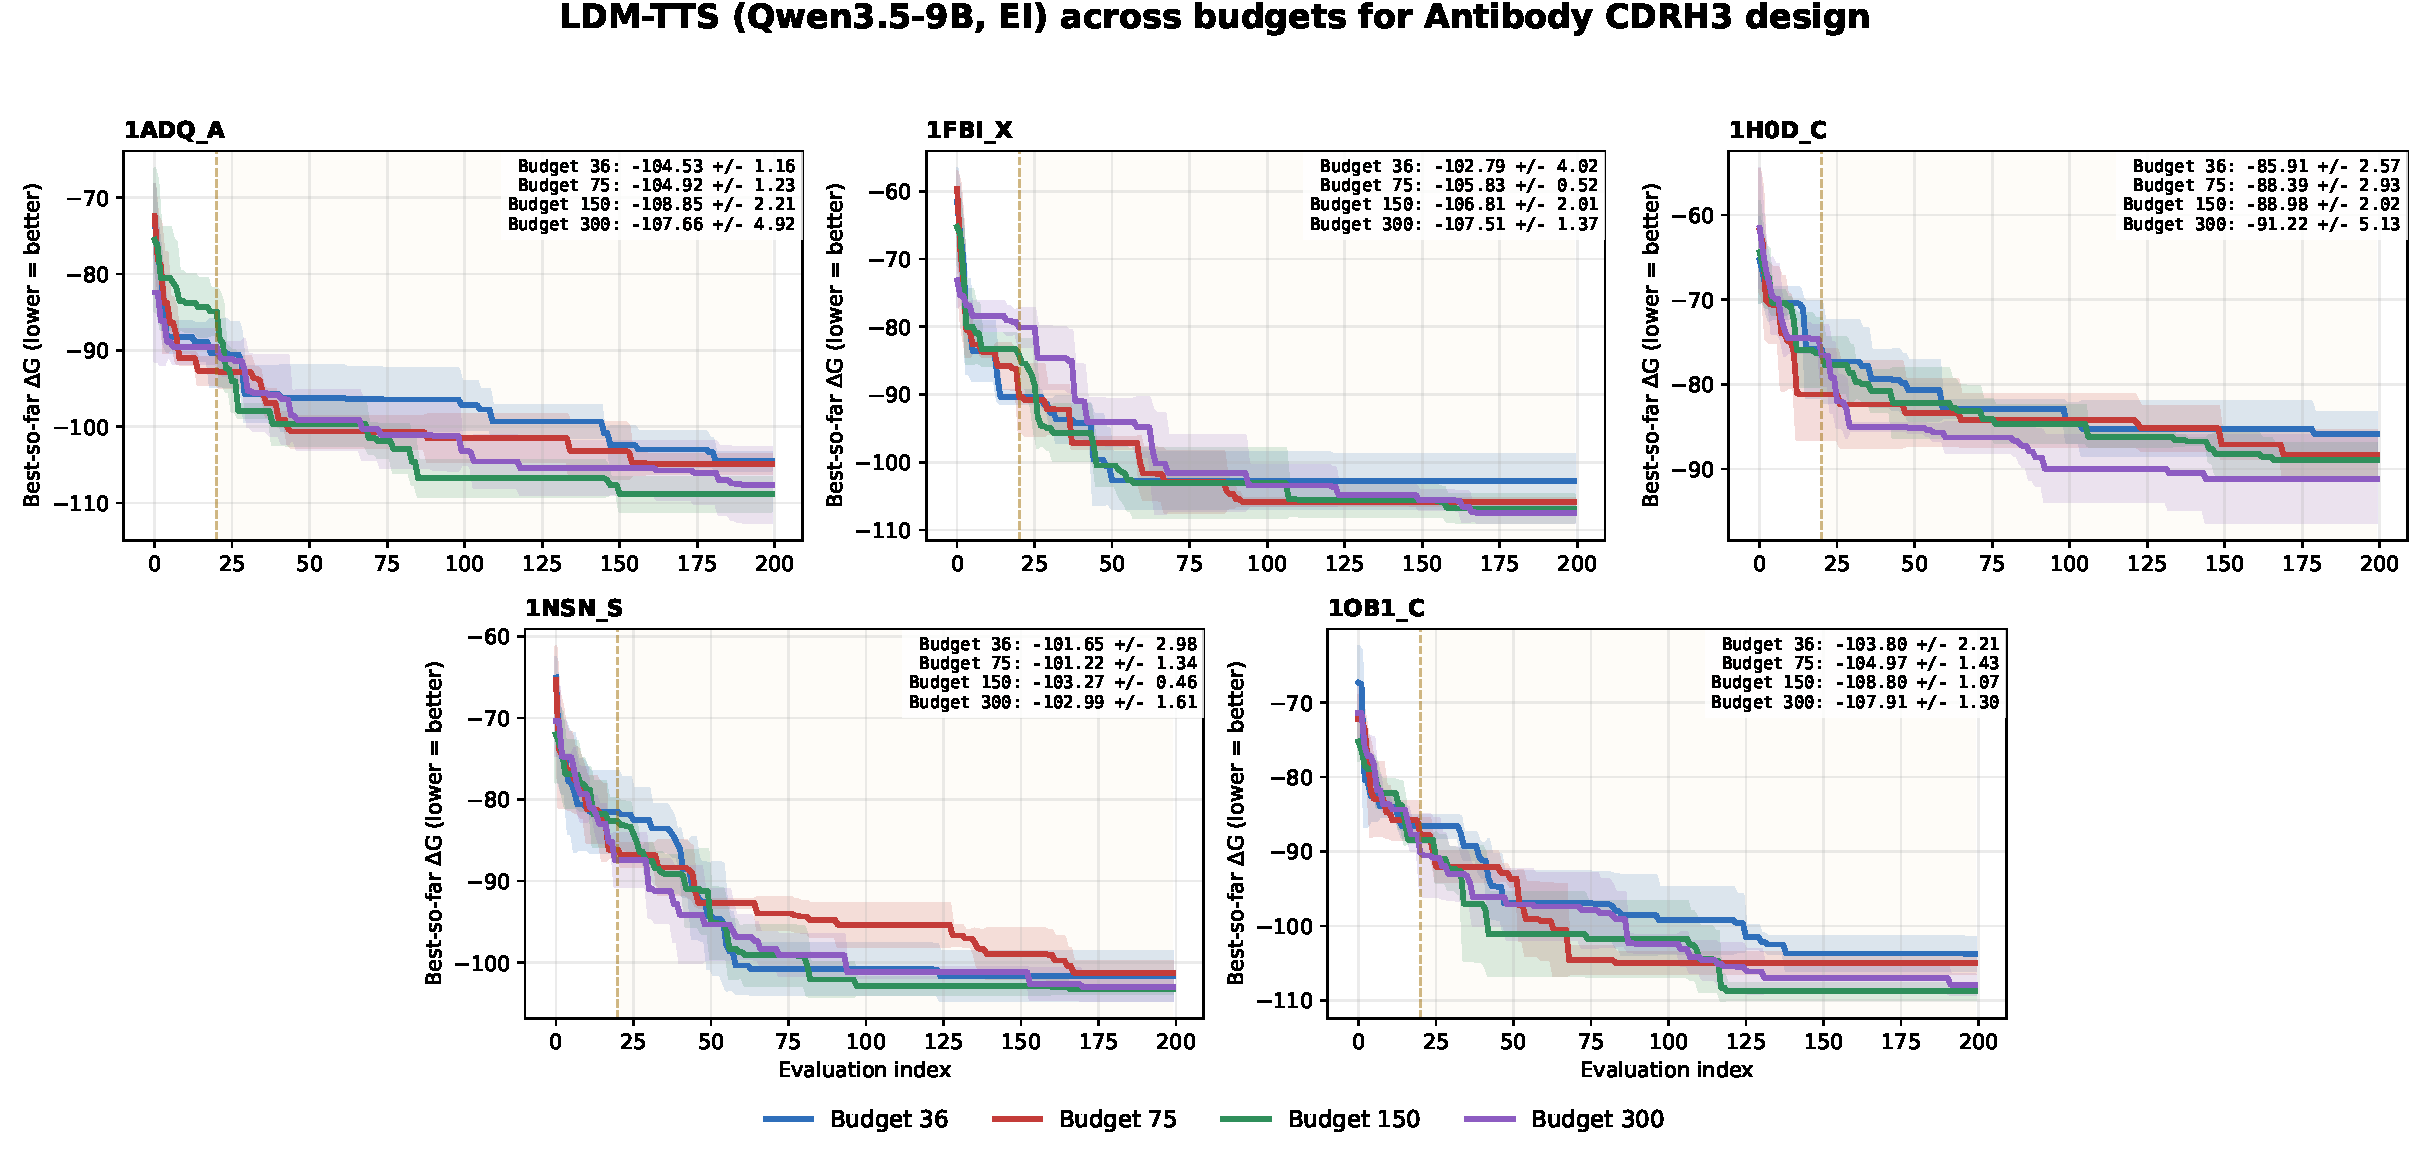
\includegraphics[width=\linewidth]{figure/ei_budget_comparison_5subplots.pdf}
    \caption{Effect of LDM-TTS proposer budget scaling on Antibody CDRH3 design. Each budget denotes the number of candidate sequences or sequence-neighbourhood samples generated before an expensive oracle evaluation. Larger inference-time proposal budgets improve the attainable binding-energy plateau across antigen targets.}
    \label{fig:abl-antigen-tts}
\end{figure}

Figure~\ref{fig:abl-antigen-acquisition} compares different acquisition functions on the five antigens at a fixed proposer budget of $300$. LDM's calibrated acquisitions (EI, UCB and variants) are broadly better than mean-style and random baselines, mirroring the molecular trend above. The result shows that a calibrated acquisition still extracts value from a broader candidate pool even when the open-source LLM has only weak biological priors, and qualifies the §6.5.2 antibody observation: hyperparameter sweeps have only weak sensitivity in this regime, but the choice of acquisition function still matters once the BO side has enough candidates to screen.

The CDRH3 ablation is the sequence-design counterpart of the molecular budget-scaling experiment. The outer oracle budget is again fixed, but here the design space is a known, sparse, discrete sequence space rather than an open-ended SMILES space. We therefore ask a narrower question: does the LDM-TTS proposer budget on its own improve the best sequence found? A label \texttt{Budget} \(N\) denotes an inner proposer budget of \(N\) candidate CDRH3 sequences or neighbourhood samples generated before the next expensive oracle query. The CDRH3 ablation fixes the BO inner-loop side at its maximum feasible setting: after validity checks, deduplication, and history filtering, the acquisition is allowed to score all remaining candidates. So the experiment changes only the cheap LLM-side proposal breadth, not the number of oracle evaluations.

Figure~\ref{fig:abl-antigen-tts} shows the budget effect across antigen landscapes, which is weaker than that observed in molecular design. The smallest budget, \texttt{Budget} $36$, improves quickly at the beginning but usually reaches a higher plateau. Increasing the proposer budget to $75$ already improves the final binding energy on most targets, and the larger $150$ and $300$ budgets give the best final result on all five antigens. The strongest setting is target-dependent: budget $150$ is best on 1ADQ\_A, 1NSN\_S, and 1OB1\_C, while budget $300$ is best on 1FBI\_X and 1H0D\_C. This non-monotonicity is expected in a rugged sequence landscape with finite seeds and a noisy surrogate: after the acquisition has enough candidates to cover the useful local neighbourhoods, further expansion can add redundant or lower-quality regions as well as genuinely novel ones. The main conclusion is therefore not that the largest budget always wins, but that the low-budget regime is systematically acquisition-starved and that moderate-to-large test-time pools substantially lower the attainable binding-energy plateau.

This result complements the main CDRH3 comparison in Figure~\ref{fig:cs-antibody-results}. There, policy-mode LDM outperforms direct token-level generation because the open-source LLM has a weaker biological sequence prior than it has for code or SMILES; emitting a few complete CDRH3 loops does not expose enough useful reservoir mass for BO to exploit. The ablation here isolates what happens once the LDM pipeline can expand the candidate pool: additional inference-time candidates become useful precisely because they are not selected by language plausibility alone. They are filtered by the surrogate acquisition, which converts a larger discrete reservoir into stronger best-so-far binding energy without spending extra oracle calls.

Together, the molecule and CDRH3 ablations show that test-time scaling for single-step design is useful only when the added samples are exposed to a calibrated value model. Richly pretrained SMILES models can absorb large direct proposal batches; sparse biological sequence spaces need enough sequence or neighbourhood coverage before acquisition filtering becomes effective. This complements the nanoGPT ablation: in multi-turn code search, LDM-TTS improves by searching a changing program landscape; in single-step design, it improves by scaling the candidate pool a calibrated acquisition can choose from.

\begin{figure*}[t]
    \centering
    \begin{subfigure}[t]{0.48\textwidth}
        \centering
        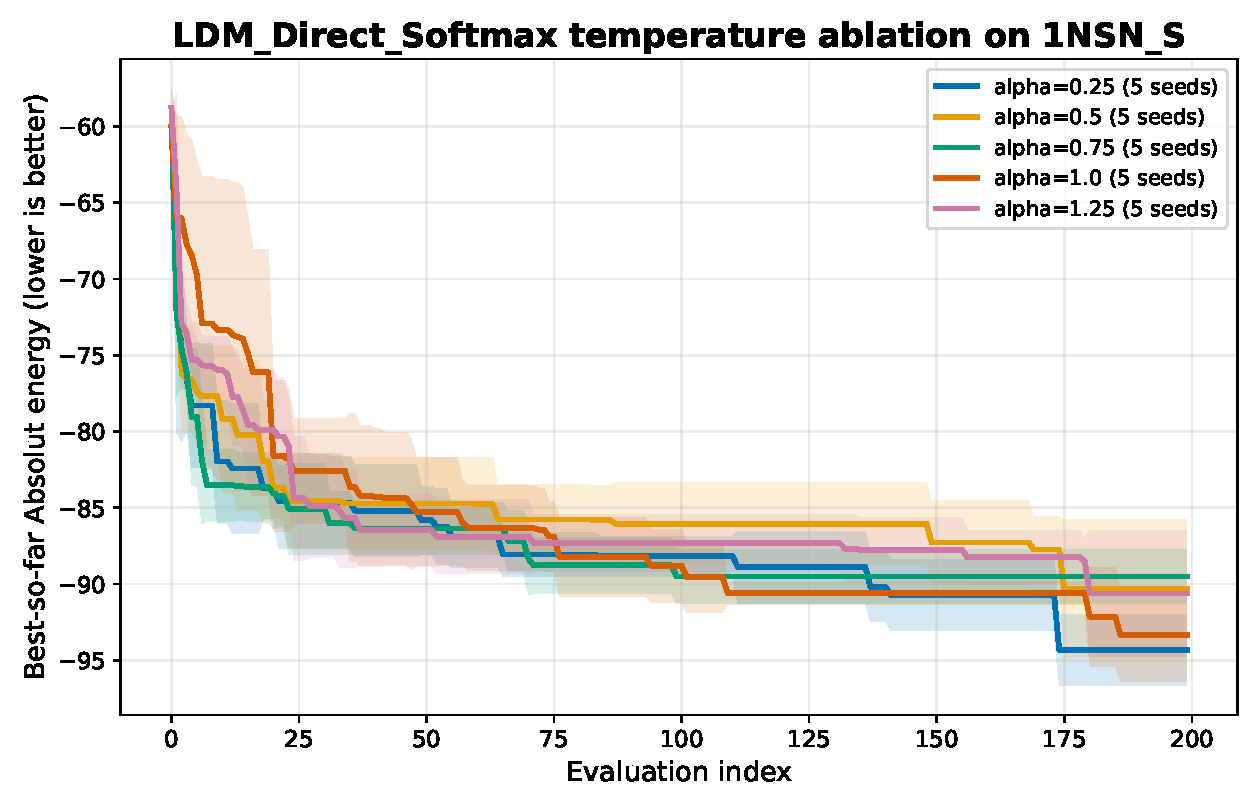
\includegraphics[width=\linewidth]{figure/ldm_direct_softmax_temperature_ablation_1NSN_S.pdf}
        \caption{Effect of the LLM sampling temperature $\alpha$ in LDM\textsubscript{Direct}\textsubscript{Softmax}. The acquisition temperature is fixed to $\eta=1$.}
        \label{fig:ablation-direct-temperature}
    \end{subfigure}
    \hfill
    \begin{subfigure}[t]{0.48\textwidth}
        \centering
        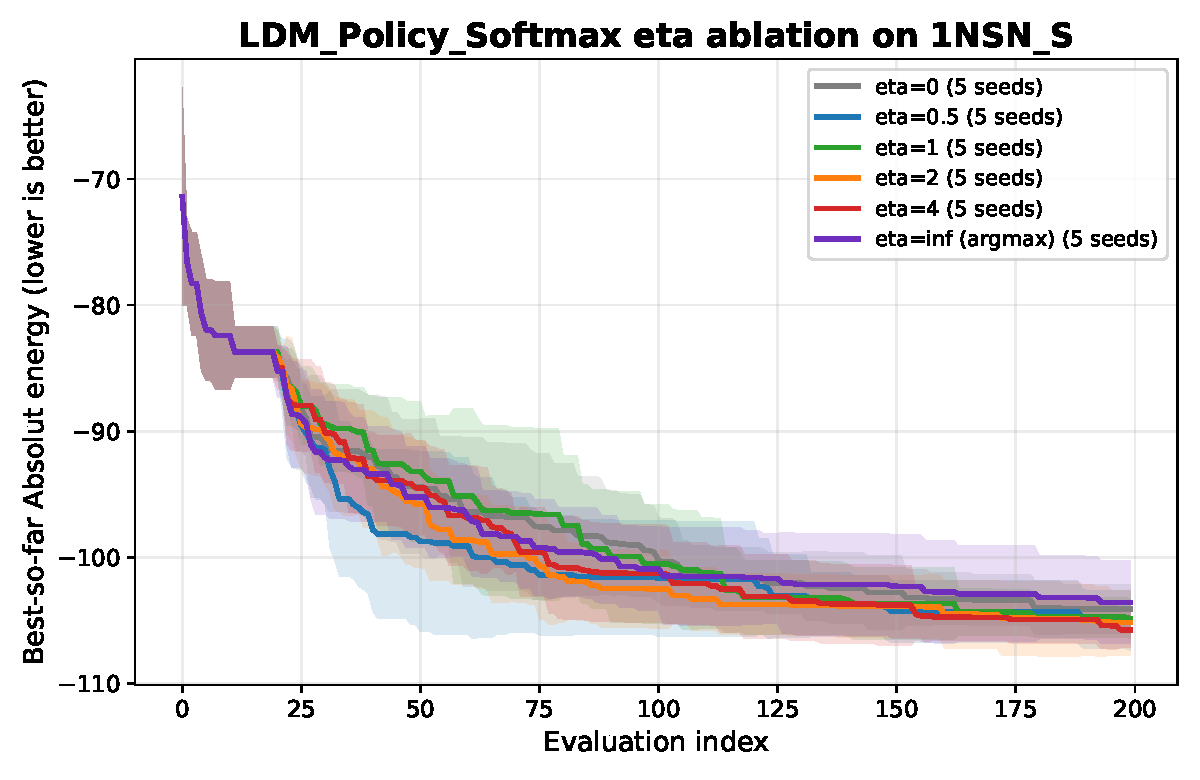
\includegraphics[width=\linewidth]{figure/ldm_policy_softmax_eta_ablation_1NSN_S.pdf}
        \caption{Effect of the acquisition temperature $\eta$ in LDM\textsubscript{Policy}\textsubscript{Softmax}. The LLM sampling temperature is fixed to $\alpha=1$.}
        \label{fig:ablation-policy-eta}
    \end{subfigure}

    \caption{Hyperparameter ablations on the antibody-design task $1\mathrm{NSN\_S}$. Each curve reports the mean best-so-far Absolut energy over five random seeds, with the shaded region showing one standard deviation. Lower values are better.}
    \label{fig:hyperparameter-ablations}
\end{figure*}

\subsection{Hyperparameter ablations for LDM.}
\label{app:abl-hyper-ldm}

We here supplement the sensitivity analysis of the two LDM variants on antigen $1\mathrm{NSN\_S}$ using five random seeds. For LDM\textsubscript{Direct}\textsubscript{Softmax}, we vary the LLM sampling temperature $\alpha\in\{0.25,0.5,0.75,1,1.25\}$ while fixing the acquisition temperature to $\eta=1$. For LDM\textsubscript{Policy}\textsubscript{Softmax}, we fix $\alpha=1$ and vary the acquisition temperature $\eta\in\{0,0.5,1,2,4,\infty\}$. Here, $\eta=0$ corresponds to uniform selection among the policy representatives, while $\eta=\infty$ is equivalent to acquisition-function argmax. The per-temperature curves are plotted in Figure~\ref{fig:hyperparameter-ablations}; we discuss their interpretation below.

This overall behaviour is consistent with the discussion in Section~\ref{sec:ablation-main}. Figure~\ref{fig:hyperparameter-ablations} shows the per-temperature curves. The open-source LLM lacks biological sequence domain priors, so its autoregressive proposals over the $20^{11}$ CDRH3 space are effectively near-random; in the policy variants the LLM already implements an implicit form of acquisition-aware importance sampling by expanding the candidate neighbourhood around promising incumbents rather than committing to a single sequence, which dampens the marginal effect of further reweighting at test time. Consequently, global sweeps over the sampling temperature $\alpha$ and the acquisition temperature $\eta$ on antigen $1\mathrm{NSN\_S}$ produce only weak sensitivity: Direct-Softmax slightly favours low $\alpha$ and Policy-Softmax shows a marginal edge near $\eta=4$, but all error bars overlap. Adjusting the two temperature knobs does not significantly change the final binding energy, which is consistent with the observation in \S\ref{sec:cs-antibody-results} that the policy-mode LDM gain over direct generation comes from the LLM's structural priors rather than from acquisition reweighting alone.
% ============================================================
\begin{figure}[t]
\centering
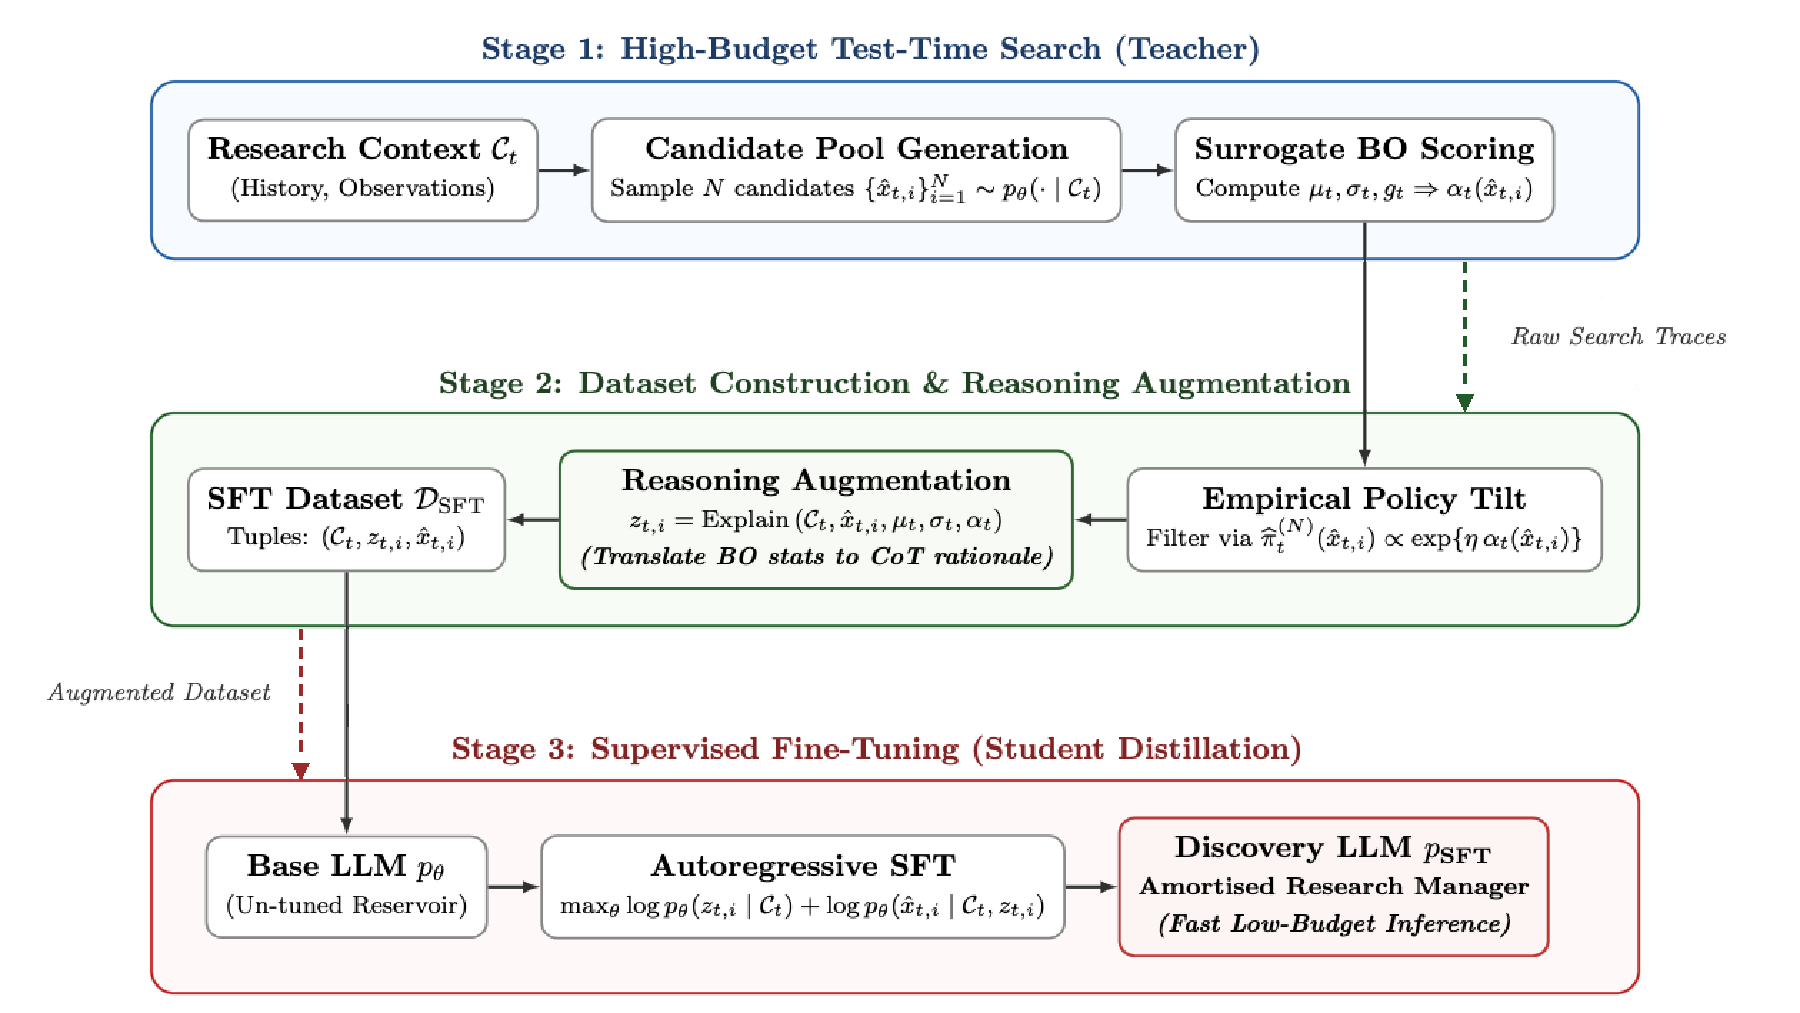
\includegraphics[width=1\textwidth]{figure/workflow.pdf}
\caption{\textbf{Overview of the LDM training pipeline workflow.}
\textbf{Stage 1:} High-budget test-time search generates candidate pools scored
by surrogate acquisition values ($\alpha_t$). \textbf{Stage 2:} High-value
candidates are filtered via an empirical policy tilt $\widehat{\pi}_t^{(N)}$,
and numerical BO statistics are translated into semantic reasoning rationales
($z_{t,i}$) via reasoning augmentation. \textbf{Stage 3:} The base model is
fine-tuned on the CoT target $(z_{t,i}, \hat{x}_{t,i})$ using standard
next-token prediction, compiling the high-budget search policy into an
amortised student model ($p_{\text{SFT}}$) capable of fast, low-budget
inference.}
\label{fig:app-training-pipeline}
\end{figure}

\section{Additional Fine-Tuning Analyses}
\label{app:finetuning-details}
% ============================================================

Section~4.4 describes how high-budget LDM test-time search is distilled into a
student proposer, and Section~6.4 reports the main fine-tuning results on
AutoResearch, antibody design, and small-molecule discovery. This appendix
provides complementary evidence that is not repeated in the main text.

\subsection{Fine-Tuning as Value Distillation}
\label{app:finetune-values}

Modern LLM fine-tuning paradigms can be distinguished by the
decision-theoretic value they distill into the model weights. Chat LLMs distill
human preference value, reasoning LLMs distill verification value, and
Discovery LLMs distill epistemic acquisition value. The object distilled by
LDM is therefore not the measured reward $R(x)$ alone, nor the static
memorisation of a high-reward molecule, protein, or program. Instead, the goal
is to distill the acquisition strategy that decides which scarce experiment is
worth running under uncertainty. Figure~\ref{fig:app-training-pipeline} summarises this three-stage training pipeline: high-budget test-time search, reasoning-augmented dataset construction, and supervised distillation into the student proposer.


Table~\ref{tab:reasoning-augmentation} illustrates how numerical acquisition
evidence is translated into semantic supervision across the three discovery
domains.

\begin{table}[H]
\centering
\small
\begin{tabular}{@{}p{0.18\linewidth}p{0.36\linewidth}p{0.40\linewidth}@{}}
\toprule
\textbf{Domain} & \textbf{Acquisition evidence (Numerical)} & \textbf{Example augmented rationale (Semantic)} \\
\midrule
\texttt{autoresearch} code search &
Best run \texttt{state\_0019} reaches \texttt{val\_bpb} $0.9811$ by lowering \texttt{TOTAL\_BATCH\_SIZE} and tuning \texttt{ASPECT\_RATIO}; several near-best runs also lower the batch size. The current parent already sits at the minimum batch size with only $5$ active parameters and no improvement over the last $4$ rounds. &
Lowering the total batch size has been a robust positive move---more steps fit inside the fixed $30$\,s budget---but that lever is now exhausted and the active parameters have \textbf{plateaued over the last four rounds}, so the set is near its ceiling. Rather than re-tuning saturated knobs, I should \textbf{activate a currently-inactive parameter} (e.g.\ \texttt{MATRIX\_LR}) to open a new optimisation dimension. \\
\addlinespace
Antibody CDRH3 design &
Best sequence \texttt{ADGHTKQNPRW} at $-64.28$; the last four candidates share the fixed prefix \texttt{ADGHTKQNPR} and scan only the final position (W $-64.28$, Y $-62.69$, A $-59.38$, S $-57.96$). &
The history is a single-point scan of the last residue on an already-refined scaffold, with the bulky aromatic W best so far. The informative move is to keep the refined prefix and test an \textbf{untested residue of similar hydrophobic character}---leucine (L)---which may reproduce W's favourable hydrophobic contact; propose \texttt{ADGHTKQNPRL}. \\
\addlinespace
Small-molecule discovery &
$29$ molecules evaluated and the loop is flagged \texttt{stalled}; the top actives ($\sim\!8.1$) share one isoxazolone/thiazolone fused core with isopropoxy and cyano groups, docking $\sim\!-8$. &
Because the loop is stalled and near-duplicates are disallowed, adding a methyl to a known winner carries no information. The higher-value move is a \textbf{recombination or scaffold hop}---e.g.\ combining the pyridine-ring variant with the morpholine side chain into a molecule not yet seen---so the candidate probes a genuinely new region of the Pareto frontier rather than exploiting a saturated one. \\
\bottomrule
\end{tabular}
\vspace{0.5em}
\caption{\textbf{Reasoning augmentation turns numerical acquisition labels into semantic training signals.}
The rationales are faithful (translated and condensed) excerpts of reasoning traces generated by the self-hosted DeepSeek V4 Flash teacher inside the high-budget LDM-TTS loop, one per domain. They describe the epistemic value of managing research progress by reading the evaluated history, diagnosing stagnation, and choosing an information-adding move, rather than focusing only on the domain-specific final solution.}
\label{tab:reasoning-augmentation}
\end{table}

\subsection{Cross-Molecule Transfer without Reasoning Augmentation}
\label{app:finetune-no-augmentation}

We test the minimal form of discovery fine-tuning without an explicit
reasoning target. Training data are collected from high-budget LDM-TTS traces
on a source molecular optimisation task. The Qwen3.5-9B proposer is fine-tuned
on acquisition-weighted examples and then evaluated on a different molecular
optimisation task within the same acquisition-guided LDM loop.

This ablation retains the same LDM state and action schema as the
reasoning-augmented setting, but omits the explicit research-progress
rationale $z_{t,i}$.

This setting shows positive transfer across molecular tasks. The base
Qwen3.5-9B LDM reaches a final hypervolume of $16.489\pm5.867$, whereas the
fine-tuned model reaches $22.279\pm3.828$ under the same evaluation protocol.
Because the discovery data are collected from one molecule and evaluated on
another, the improvement cannot be explained by memorising the final molecules
from the source task. It instead shows that acquisition-weighted fine-tuning
can transfer part of the research-management policy even without an explicit
reasoning channel.

\subsection{Supplementary Quantitative Tables}
\label{app:finetune-tables}

Table~\ref{tab:app-smallmol-cot} retains the G12C results not shown in the
main-text KRAS G12D learning curve. Table~\ref{tab:app-finetune-cot-ablation}
collects the numerical cross-domain comparison underlying the three main-text
figures.

\begin{table}[H]
\centering
\small
\begin{tabular}{@{}lcc@{}}
\toprule
\textbf{Inference policy} & \textbf{KRAS G12C} & \textbf{KRAS G12D} \\
 & HV $\uparrow$ & HV $\uparrow$ \\
\midrule
Qwen3.5-9B base (without\_cot) & $11.64\pm2.63$ & $16.49\pm5.87$ \\
Fine-tuned Qwen3.5-9B (without\_cot) & $14.73\pm3.09$ & $22.28\pm3.83$ \\
DeepSeek V4 Flash (without\_cot) & $18.97\pm1.76$ & $24.55\pm3.59$ \\
DeepSeek V4 Flash (with\_cot) & $19.98\pm2.00$ & $24.07\pm3.12$ \\
\textbf{Fine-tuned Qwen3.5-9B (with\_cot)} & $\mathbf{20.98\pm2.92}$ & $\mathbf{26.66\pm2.61}$ \\
\bottomrule
\end{tabular}
\caption{\textbf{Reasoning-augmentation ablation on small-molecule discovery.}
Final Pareto-front hypervolume at an evaluation budget of 80, averaged over five seeds.}
\label{tab:app-smallmol-cot}
\end{table}

\begin{table}[H]
\centering
\setlength{\tabcolsep}{4pt}
\scriptsize
\begin{tabular}{@{}lcccc@{}}
\toprule
\textbf{Model} & \textbf{CoT} & \textbf{AutoResearch} & \textbf{Antibody} & \textbf{SmallMol} \\
 & & val\_bpb $\downarrow$ & $-E_{\mathrm{bind}}$ $\uparrow$ & HV $\uparrow$ \\
\midrule
Base Qwen3.5-9B & off & $0.9965$ & $102.6$ & $16.49$ \\
Base Qwen3.5-9B & on  & $0.9825$ & $104.4$ & --- \\
LDM-SFT & off & $0.9829$ & $105.1$ & $22.28$ \\
\textbf{LDM-SFT} & \textbf{on} & $\mathbf{0.9788}$ & $\mathbf{105.5}$ & $\mathbf{26.66}$ \\
\midrule
\multicolumn{2}{@{}l}{Qwen3-Coder-30B ref.} & $0.9801$ & --- & --- \\
\bottomrule
\end{tabular}
\caption{\textbf{Cross-domain reasoning-augmentation ablation.}
Terminal metrics for the three fine-tuning studies.}
\label{tab:app-finetune-cot-ablation}
\end{table}

\subsection{In-Distribution Single-Task Fit}
\label{app:finetune-indistribution}

Before evaluating the distilled policies in the acquisition loop, we verify
that each single-task model fits its reasoning-augmented training data. We
track training and held-out losses for \texttt{autoresearch} program search,
small-molecule KRAS design, and antibody CDRH3 design. All three losses
converge within a few dozen steps, while the held-out curves closely track the
training curves. The absolute held-out losses differ by domain: $0.06$ for
\texttt{autoresearch}, $0.38$ for small-molecule design, and $0.70$ for
antibody CDRH3 design. These differences reflect the different action spaces
and target lengths, rather than a failure to fit the data.

\begin{figure}[H]
\centering
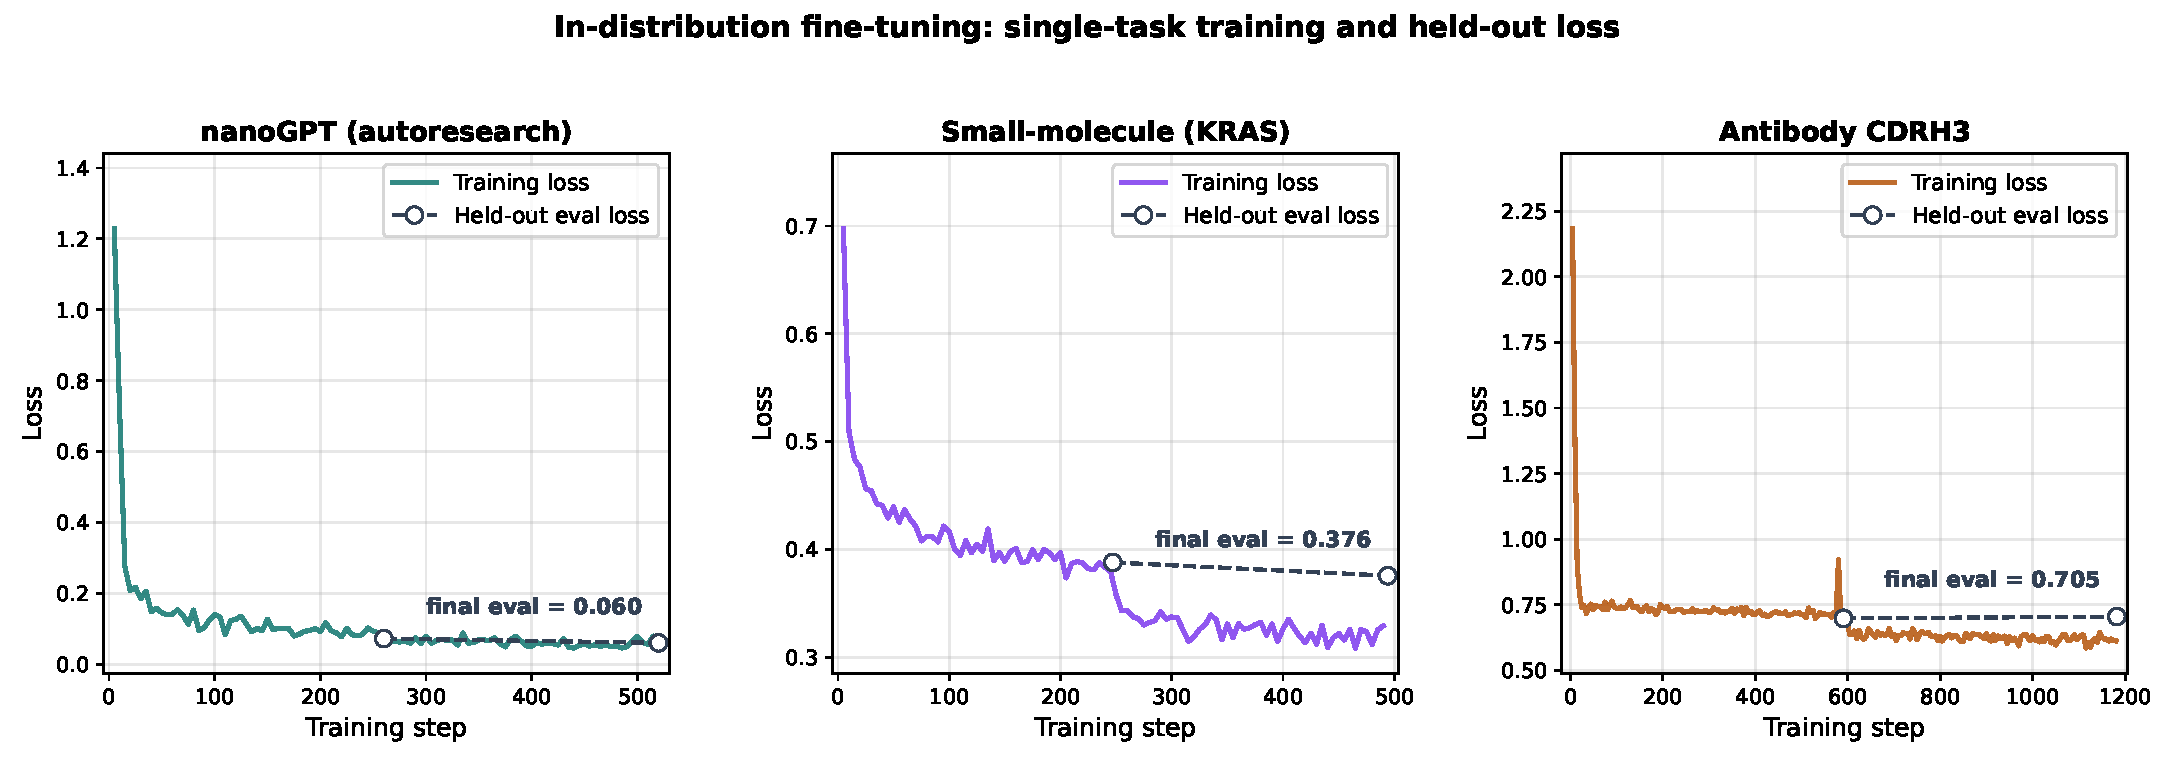
\includegraphics[width=0.95\linewidth]{figure/indist_curves.pdf}
\caption{\textbf{In-distribution single-task fine-tuning.} Training loss
(solid) and held-out evaluation loss (markers) versus training step for the
\texttt{autoresearch}, small-molecule, and antibody CDRH3 policies. All three
converge within a few dozen steps, and the held-out loss tracks the training
loss, confirming a faithful in-distribution fit before acquisition-loop
evaluation.}
\label{fig:app-indist-curves}
\end{figure}

\subsection{Out-of-distribution generalisation to held-out antigens}
\label{sec:finetune-ood}

To test whether it learns
a \text{transferable} acquisition policy rather than memorising antigen-specific patterns, we hold two of the
five antibody targets (\texttt{1FBI\_X}, \texttt{1H0D\_C}) out of training entirely, fine-tune the mixed-task
model on the other three, and evaluate on the held-out pair inside the same acquisition-guided loop, antigens
whose sequences and binding landscapes were never seen during training.

Figure~\ref{fig:protein-ood-mixed32} shows the out-of-distribution model matches or exceeds the
\emph{in-distribution} model (which \emph{was} trained on these antigens) on both held-out targets, and clearly
beats base Qwen3.5-9B with and without chain-of-thought: it reaches $-110.57$ on \texttt{1FBI\_X}
(base $-109.5$, in-distribution $-113.4$) and $-95.4$ on \texttt{1H0D\_C}, where it even surpasses the
in-distribution model ($-94.6$) and the base ($-90.9$). Since the model never observed these antigens, the gain
cannot be memorisation---the distilled acquisition policy transfers to unseen targets. 

\begin{figure}[H]
\centering
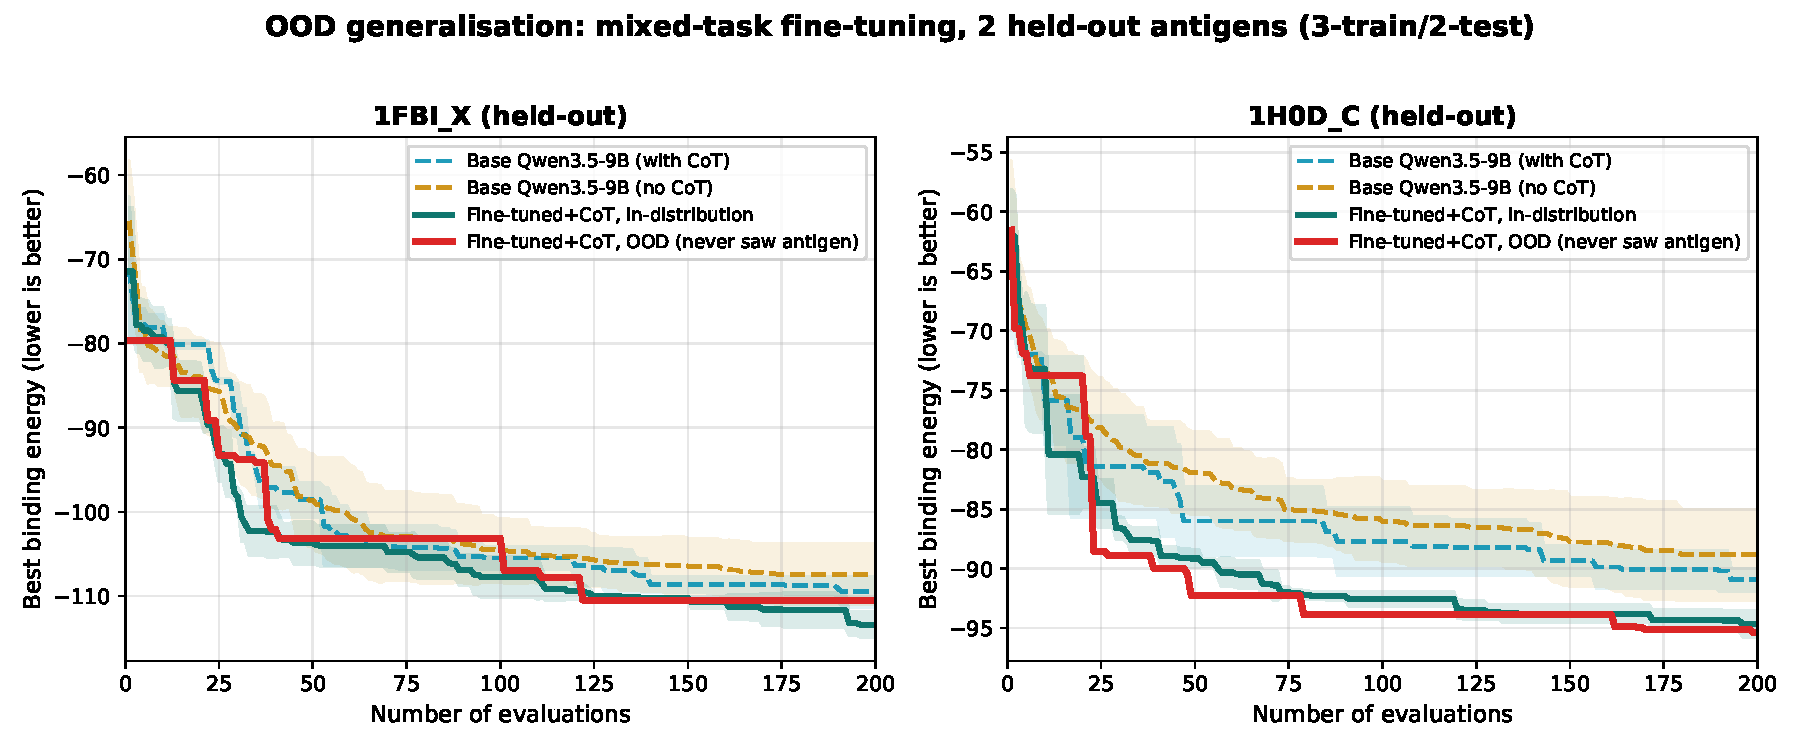
\includegraphics[width=0.98\linewidth]{figure/ood_mixed32.pdf}
\caption{\textbf{Out-of-distribution generalisation to held-out antigens (3-train/2-test).} Best Absolut binding
energy versus number of evaluations on the two held-out antigens. The mixed-task fine-tuned model evaluated on
antigens it never saw during training (red) matches or exceeds the in-distribution fine-tuned model (teal) and
clearly beats base Qwen3.5-9B with and without chain-of-thought (dashed).}
\label{fig:protein-ood-mixed32}
\end{figure}


\end{document}
